\chapter{海铃探路者实验}
\label{chap:pathfinder}

海铃探路者计划\cite{TRIDENT_pathfinder:2022}旨在为海铃大阵列的建设进行台址勘测以及技术演练。
在对南海地址结构和洋流情况进行深入的排查后,我们决定选取南海永兴岛西北处的深海平原作为未来中微子阵列的建设点,其选址的位置如图\ref{fig:pathfinder_map}所示。
探路者项目于2020年年末开启,于2021年夏季9月份前往望远镜选址处开展实地勘探实验。

\begin{figure}[htb]
    \centering
    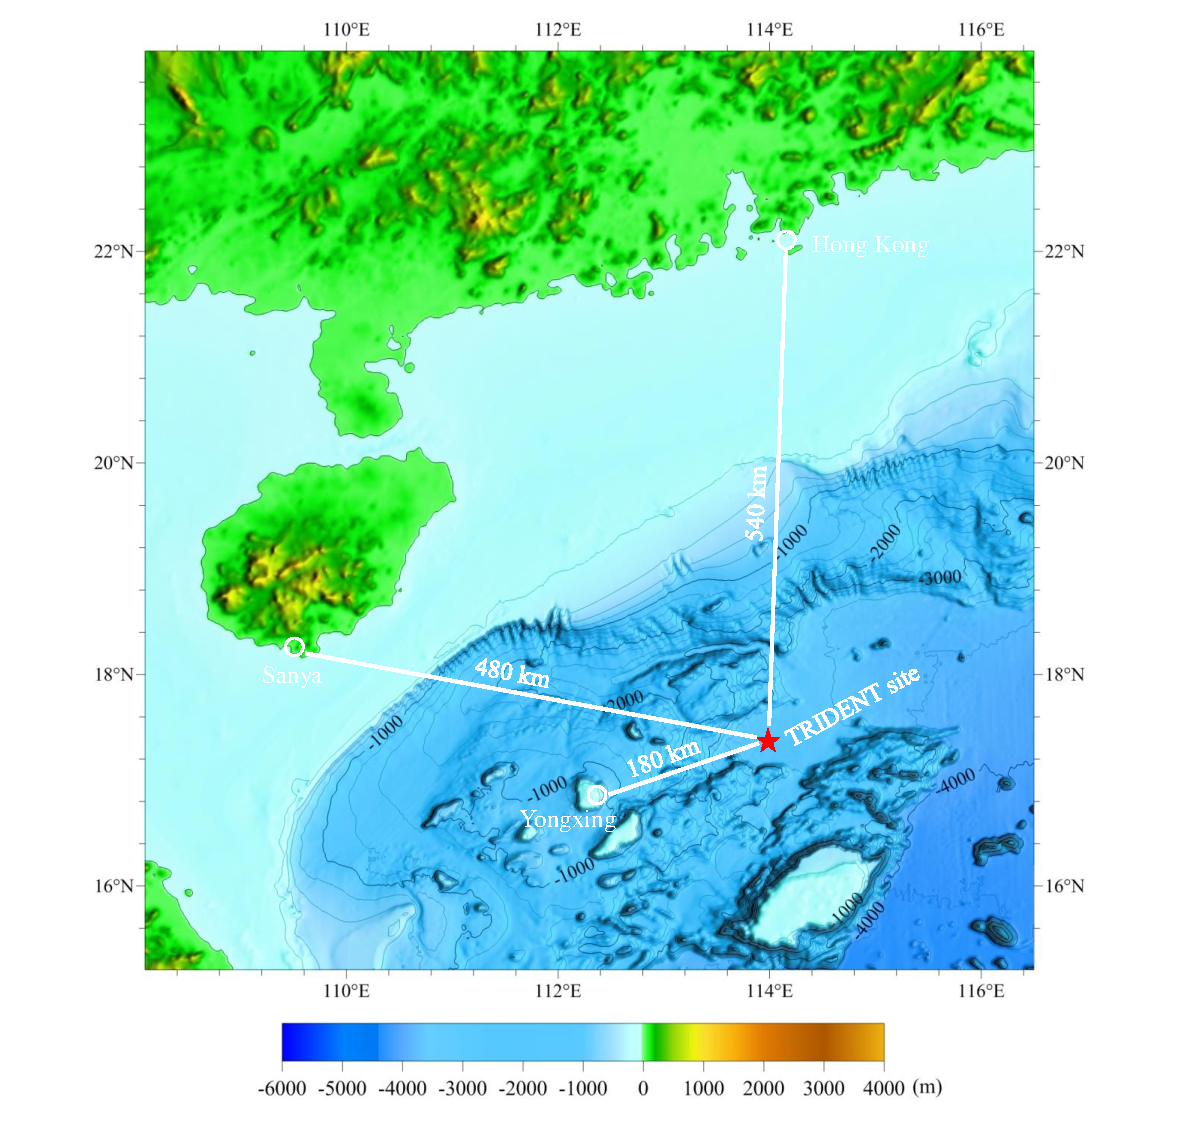
\includegraphics[width=0.8\linewidth]{img/pathfinder_map.pdf}
    \caption{海铃探路者实验位置(红色星星)以及其附近的地理环境,实验地点距离永兴岛约$180\,\mathrm{km}$。}
    \label{fig:pathfinder_map}
\end{figure}

海铃探路者项目搭乘向阳红3号科考船在南海指定台址处进行了海底地形扫描,水下的温度,盐度,密度和洋流在各个不同深度的测量(测量结果如图\ref{fig:pathfinder_ocean_condition}所示),深海海水和海床泥沙采样,以及原位海水光学性质测量等多项实验。
在下面的章节中,我们主要介绍海铃探路者的原位海水光学性质测量实验。

\begin{figure}[!htb] 
    \begin{subfigure}[!htb]{0.90\textwidth}
    \centering
        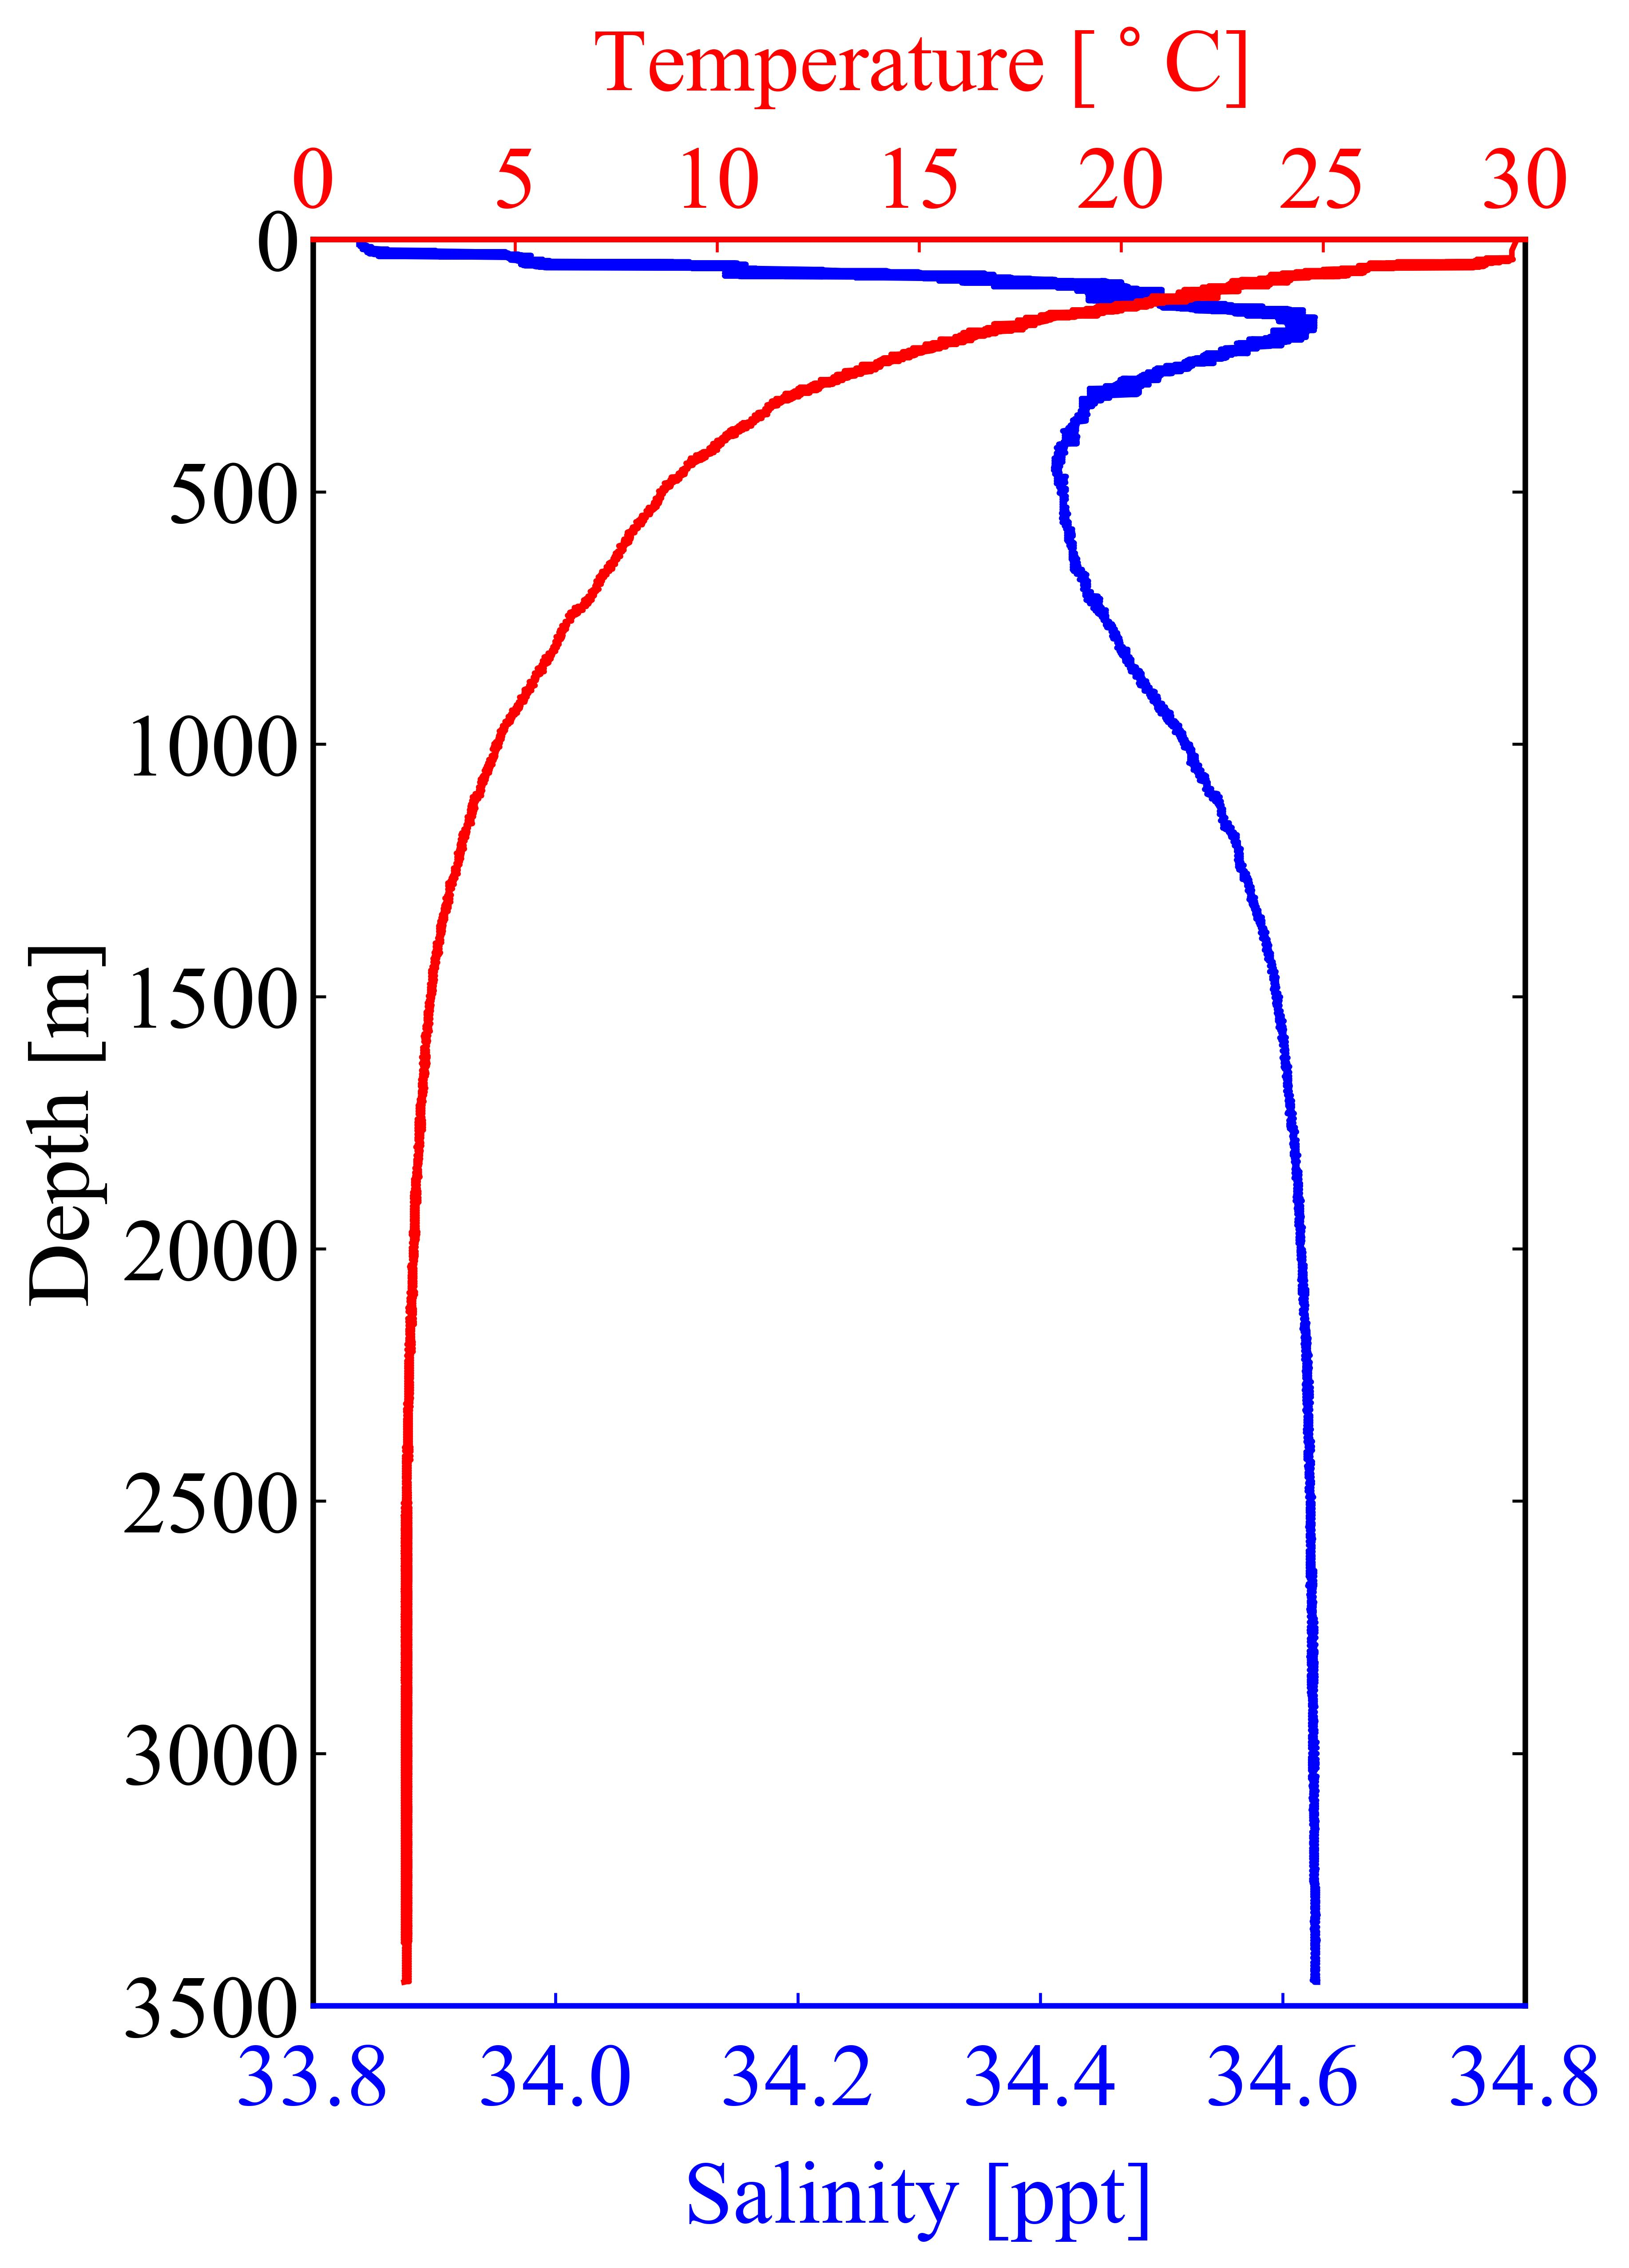
\includegraphics[width=0.44\linewidth]{img/pathfinder_temperature.jpg}
        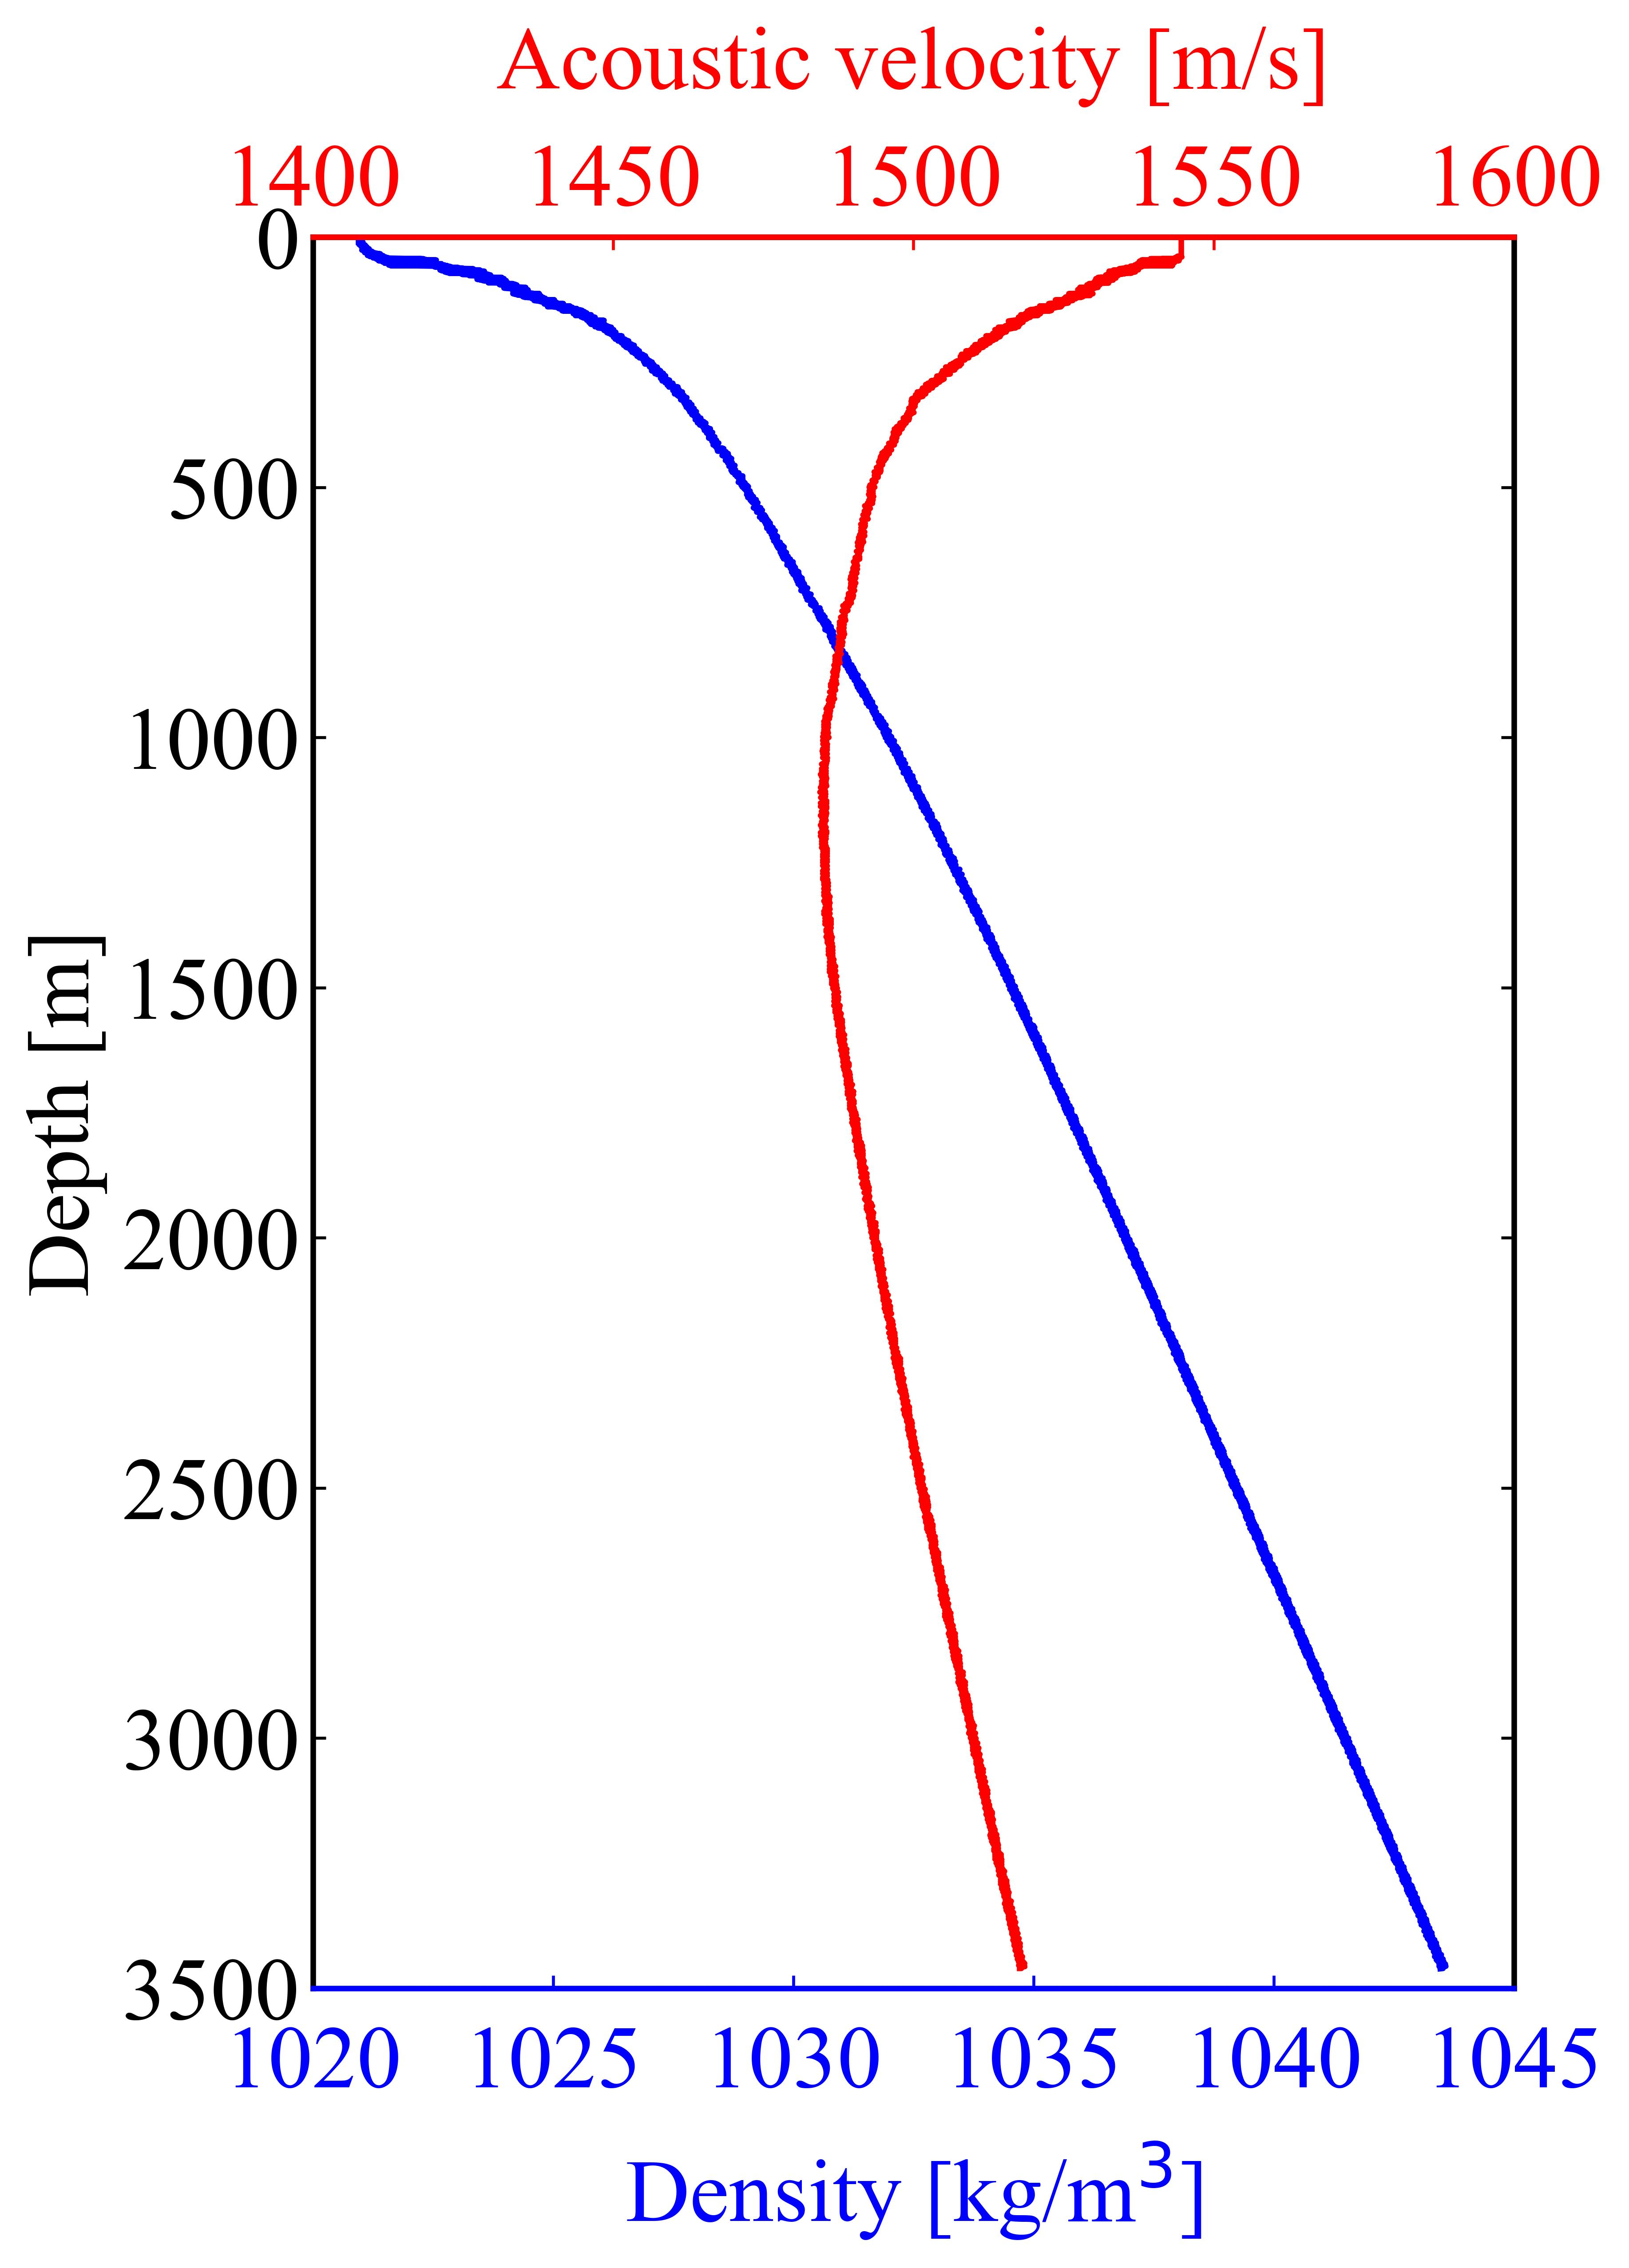
\includegraphics[width=0.44\linewidth]{img/pathfinder_sound_speed.jpg}
        \caption{左图:海水的密度和声速随深度的变化。右图:海水的温度和盐度随深度的变化。} 
    \end{subfigure}

    \begin{subfigure}[!htb]{0.90\textwidth}
        \centering
        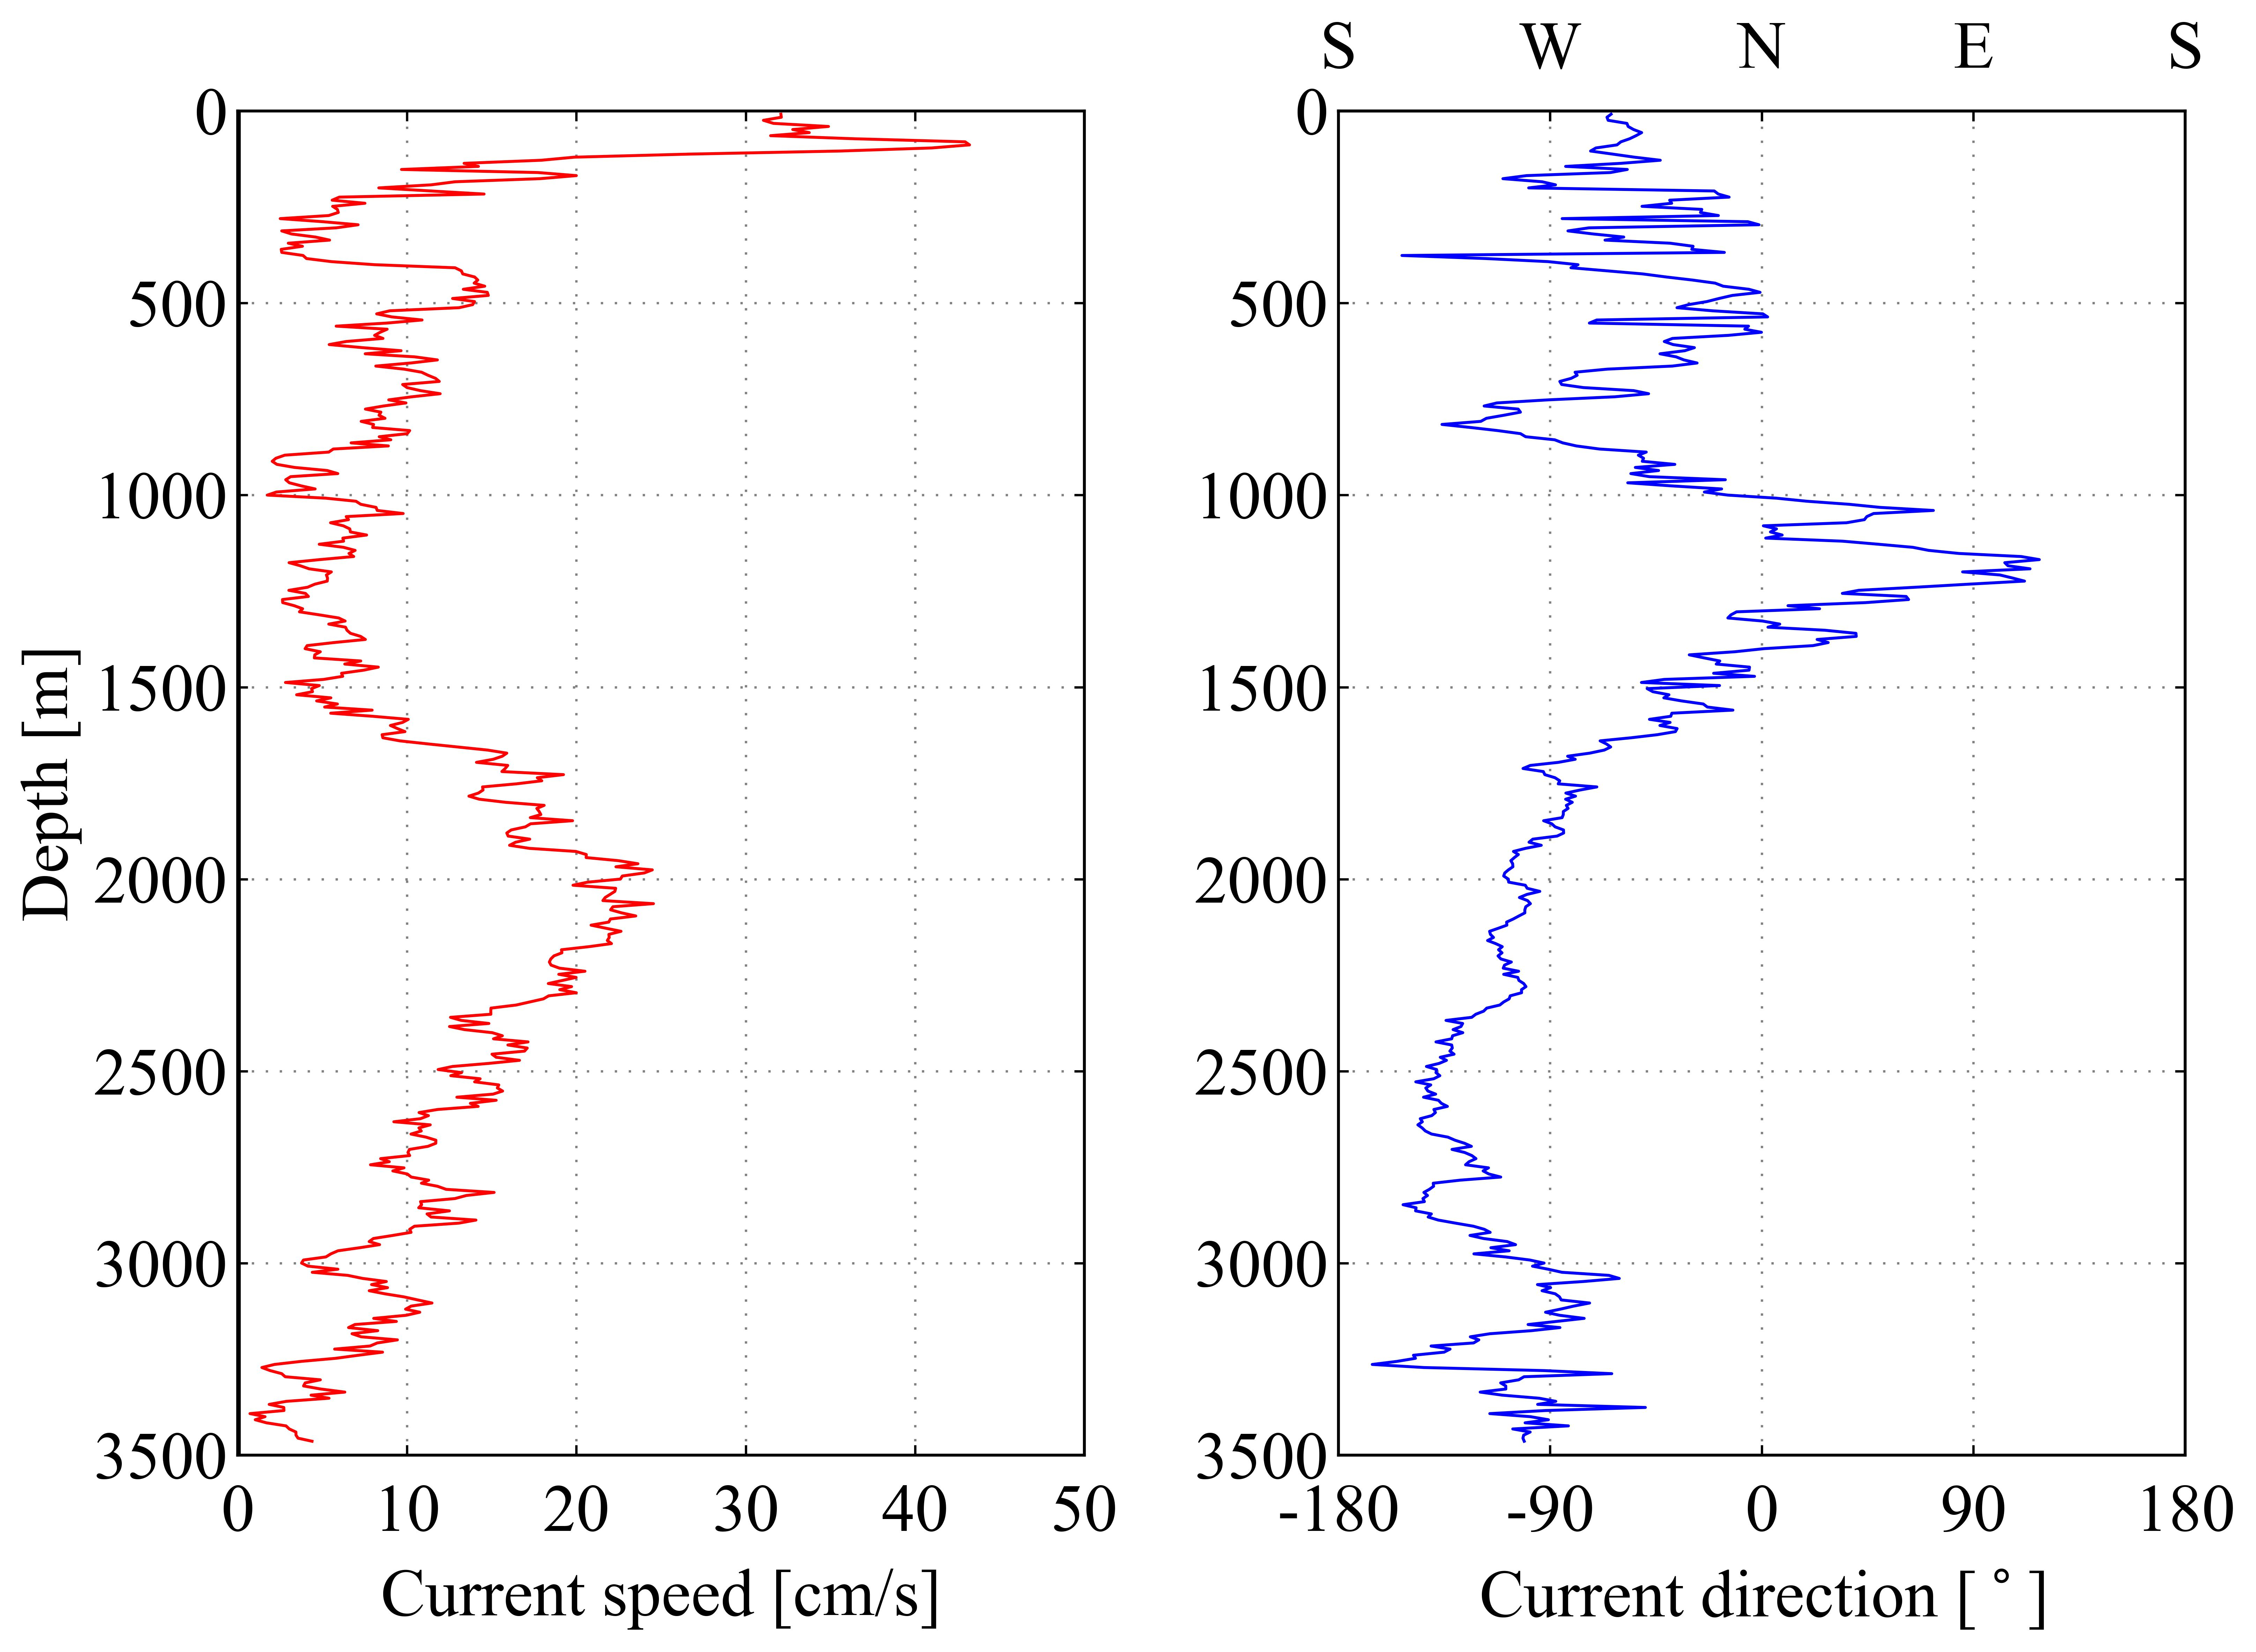
\includegraphics[width=0.90\linewidth]{img/pathfinder_current.jpg}
        \caption{左图:海水的流速大小随深度的变化。右图:海水的洋流方向随深度的变化。} 
    \end{subfigure}

    \caption{海铃探路者项目在选址处测得的海洋学数据,数据采集于2021年9月6日。}
    \label{fig:pathfinder_ocean_condition}
\end{figure}


\section{光学性质测量系统的整体设计}

海铃探路者的光学性质测量系统的目标是在深海中实现对海水光学性质的原位测量,其整体测量思路如下:在海水中放置一个光源,并在远处布置一个探测设备来观测光源,海水中的吸收和散射的效应便会映射在探测设备的观测结果上。
如图\ref{fig:pathfinder_apparatus}所示,测量系统由一个光信号发射模块和两个光信号接收模块构成(以下简称为发光球和接收球),这些模块被封装在一个17英寸的能抵抗5000米水压的玻璃球壳中。
两个接收球与发光球的距离分别为$\sim20\,\mathrm{m}$和$\sim40\,\mathrm{m}$。
通过对两个接收球测量到的结果结果进行比较,我们可以完成对海水性质的相对测量,这种相对测量的方法有助于消除一部分的系统误差。

发光球的上下两面各自包含紫($405\,\mathrm{nm}$),蓝($450/460\,\mathrm{nm}$),绿($525\,\mathrm{nm}$)3种颜色的LED。
对于每一种颜色,我们在发光球的上下两面各布置了1个处于脉冲模式下工作的LED,和5个处于常亮模式下工作的LED。
每个接收球中包含3只PMT和1个相机,当脉冲模式下的LED工作时,PMT会测量光子到达时间分布(photon arrival time distribution,以下简称为ATD),当常亮模式下的LED工作时,相机会拍摄被LED点亮的接收球的照片。
通过分析PMT测得的ATD和相机拍摄到的照片,我们可以解码出海水的光学性质。

\begin{figure}[htb]
    \centering
    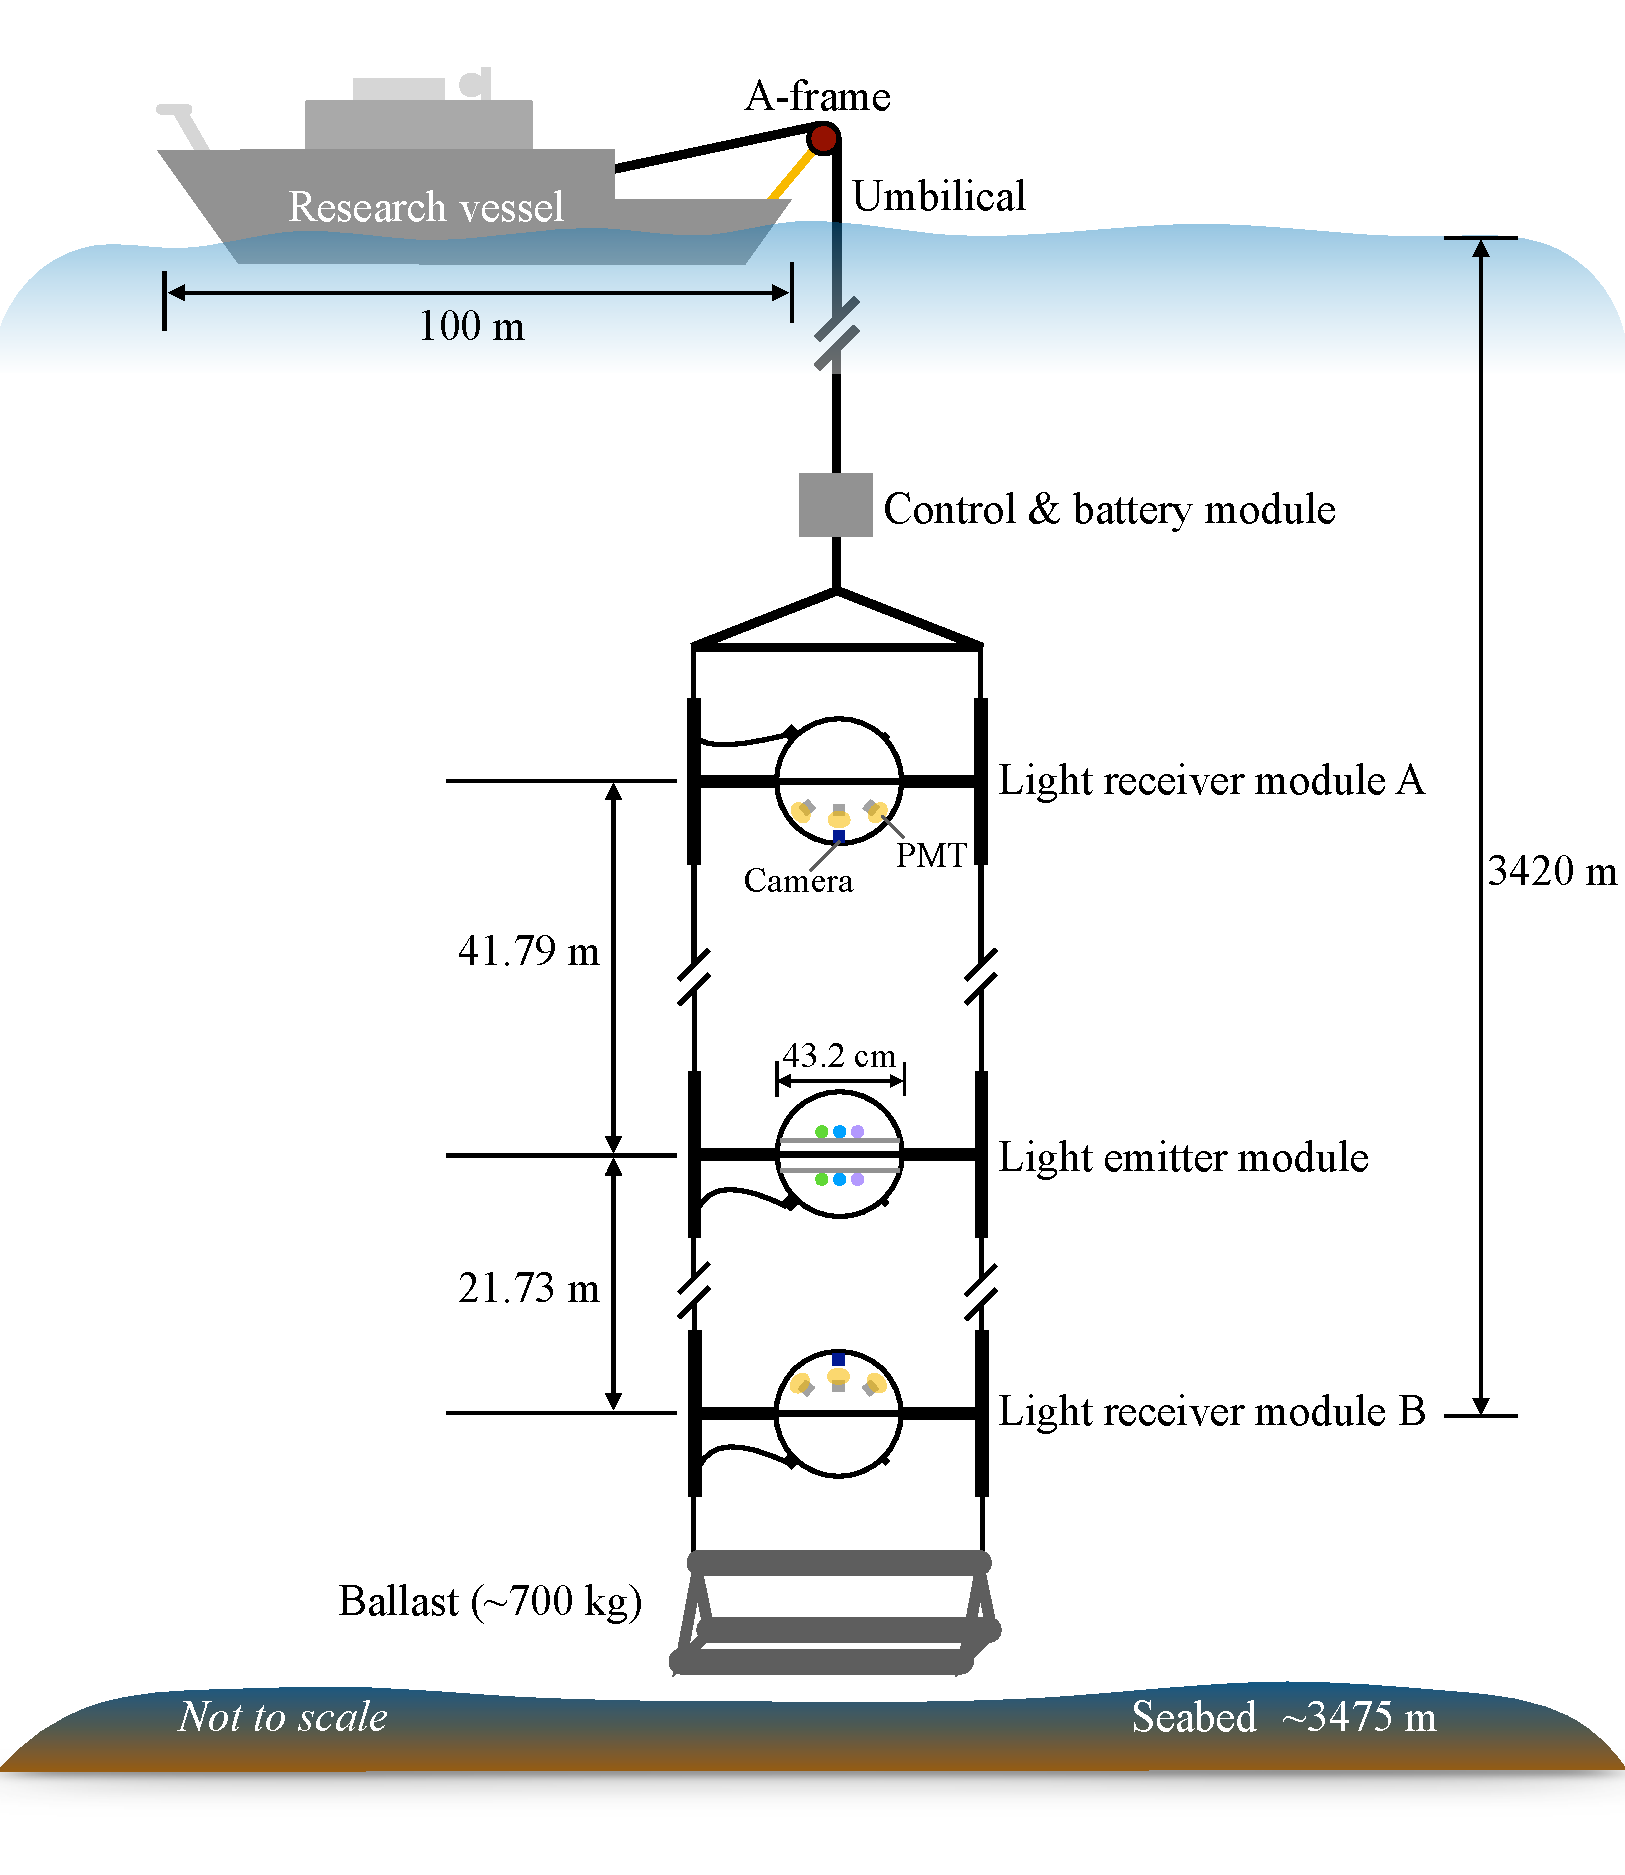
\includegraphics[width=0.85\linewidth]{img/pathfinder_apparatus.pdf}
    \caption{海铃探路者实验装置图。}
    \label{fig:pathfinder_apparatus}
\end{figure}


\section{光子传播行为的模拟研究}
\label{sec:pathfinder_sim}

海水中的吸收和散射过程总是同时存在的,他们对实验结果的可观测量的影响相互纠缠,使得我们难以直接地分别解码出吸收长度和散射长度各自的值。
由于光子的运动学特征(位置,时间和方向)在经过几次散射过程之后便很难用解析的形式定量分析,因此我们需要通过模拟手段来对其进行研究\cite{pathfinder_simulation:2022}。
通过模拟研究,我们可以对实验结果做一些预计,并且对初始阶段的实验设计思路和实验完成后的数据分析方法提出改进。

\subsection{Geant4模拟程序介绍}

我们使用了\textsf{Geant4}粒子物理模拟框架来构建了一个模拟程序\footnote{https://github.com/TRIDENT-Neutrino-Telescope/Pathfinder-Optical-Simulation},它可以模拟光子从发光球的发射,在海水中的传播,以及被探测球的接收过程。
\textsf{Geant4}框架具有模块化的结构设计,具备优秀的可拓展性,此外\textsf{Geant4}的光学物理模块\textsf{G4OpticalPhysics}中已经包含了对吸收,瑞利散射和米散射的物理描述。

在实验原本几何结构中,从发光球各项均匀发射出来的光子大部分都耗散在了广阔的海水中,实际能到达接收球的比例仅为$\sim (20\,\mathrm{cm} / 20\,\mathrm{m})^2 =10^{-4}$,其中$20\,\mathrm{cm}$表示接收球的半径,$20\,\mathrm{m}$表示接收球与发光球的距离。
考虑到在我们的实验中,发光球内部双扩散层的设计可以将LED发射出来的光子充分地弥散掉,因此发光球是一个近似各向同性的光源,而且海水的光学性质也是各向均匀的,所以在模拟程序中,我们可以对几何体做一些简化来提高模拟的计算效率。
几何简化的过程如图\ref{fig:pathfinder_sim_geo}所示,我们将接收模块从球形改成了包裹发光模块的壳形,从而确保未被吸收的光子都能被接收球所探测到,这样便能把发射出来的光子的接收效率提升到$100\%$。

在模拟程序的输入输出数据接口总结在表\ref{tab:pathfinder_sim_io}中,程序的输入为章节\ref{subsec:optical_model}中讨论过的海水的光学性质参数,而输出为光子在接收面上的动力学信息,部分符号的含义如图\ref{fig:pathfinder_sim_geo}中右侧所示。
我们使用模拟来辅助实验的整体思路便是:通过改变输入的光学性质,观察模拟结果的变化,进而研究介质的光学性质对探测器观测到的测量量的影响和使用测量量来解码出光学性质参数的方法。

\begin{figure}[htb]
    \centering
    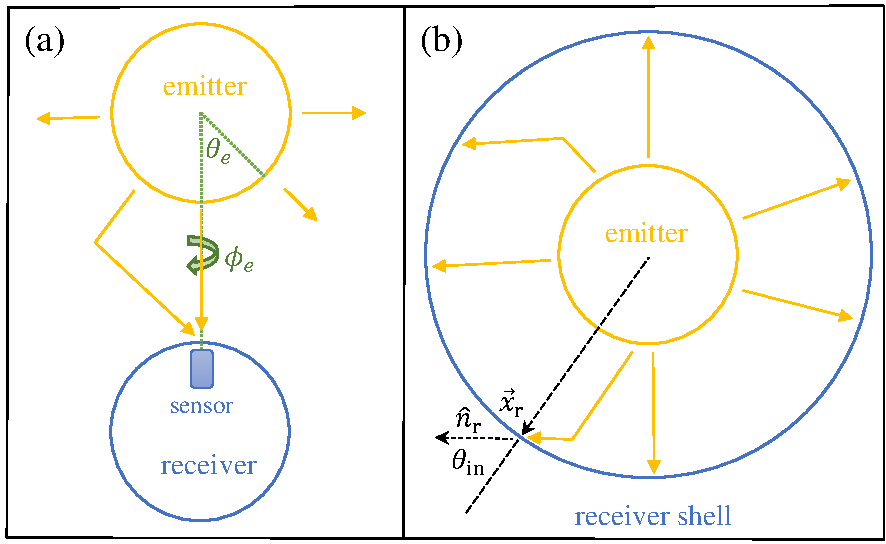
\includegraphics[width=0.85\linewidth]{img/pathfinder_sim_geo.pdf}
    \caption{实验中的几何结构(左图)和模拟中的几何结构(右图)的对比。}
    \label{fig:pathfinder_sim_geo}
\end{figure}

\begin{table}[]
    \centering
    \caption{模拟程序的输入输出接口列表}
    \label{tab:pathfinder_sim_io}
    \begin{tabular}{|c|c|c|}
        \hline
         & 变量名称 & 物理含义 \\
        \hline
        \multirow{5}{3em}{Input} 
        & $\lambda_\mathrm{abs}$ & 吸收长度  \\
        & $\lambda_\mathrm{Ray}$ & 瑞利散射长度 \\
        & $\lambda_\mathrm{Mie}$ & 米散射长度 \\
        & $\mu$ & 米散射平均散射角 \\
        & $d$ & 发光球与接收球壳之间的距离 \\
        \hline
        \multirow{5}{3em}{Output} 
        & $\vec{x}_\mathrm{e}$ & 光子发射时在发光球的位置  \\
        & $\vec{x}_\mathrm{r}$ & 光子接收时在接收球的位置 \\
        & $\hat{n}_\mathrm{r}$ & 光子接收时的运动方向 \\
        & $t$ & 光子经历的传播时间 \\
        & $k$ & 光子经历的散射次数 \\
        \hline
    \end{tabular}
\end{table}


\subsection{在模拟中复现实验测量结果}

在探路者实验中,主要的实验观测量为相机观测到的照片以及PMT观测到的ATD。通过对模拟输出的光子动力学信息做一定变换,我们可以在模拟中复现这两个观测量。
为此我们启动了两组模拟,他们的发光球和接收球的距离分别为$d_1 = 20\, \mathrm{m}$ 和 $d_2 = 40\, \mathrm{m}$。
模拟中所采用光学性质参数总结在表\ref{tab:pathfinder_sim_set},这是一组海水中典型的光学性质参数\cite{OP_ANTARES:2004, OP_P-One:2021, TRIDENT_pathfinder:2022}。
在每一组模拟中,我们都在接收球表面发射$10^7$的光子数量,从而保证后续分析中的统计性。

\begin{table}
    \centering
    \caption{模拟输入的默认光学性质的值}
    \label{tab:pathfinder_sim_set}
    \centering
    \begin{tabular}{|c|c|c|c|c|}
        \hline
        输入参数 & $\lambda_\mathrm{a}$ & $\lambda_\mathrm{Ray}$ & $\lambda_\mathrm{Mie}$ & $\langle \cos\theta \rangle$\\
        \hline
        参数值 & 27\,m & 200\,m & 70\,m & 0.97\\
        \hline
    \end{tabular}
\end{table}

对于相机拍摄照片的过程,我们可以用一个小孔成像近似来模拟光子在相机底片上成像的行为。对于我们实验采用的相机来说,相机的物距在约无穷远处,且相机的光圈较小,因此小孔成像近似可以使用。
如图\ref{fig:pathfinder_sim_cam_pinhole}所示,我们首先利用光子的动量信息来计算光子相对于接收平面的入射角$\theta_\mathrm{in}$:
\begin{equation}
    \theta_\mathrm{in} = \arccos \left( \hat{n}_\mathrm{r} \cdot \frac{\vec{x}_\mathrm{r}}{\vert\vec{x}_\mathrm{r}\vert} \right) . \label{eq:pathfinder_sim_cam_pinhole}
\end{equation}
然后我们便可以计算光子落在相机底片的半径$r_\mathrm{film}$:
\begin{equation}
    r_\mathrm{film} = f_\mathrm{lens} \sin{\theta_\mathrm{in}} , \label{eq:camera_radius}
\end{equation}
其中$f_\mathrm{lens} = 25\,\mathrm{mm}$是相机的焦距。最后再考虑到探路者中使用的CMOS底片的像素大小为$3.45\,\mu\mathrm{m}$,即单个像素对应$1.38 \times 10^{-4} \,\mathrm{rad}$的角度,由此我们可以得到光子在CMOS底片上的像素坐标。
由于我们使用的CMOS底片在探路者项目的光照强度下对光子的响应满足非常好的线性规律,因此我们可以将落在CMOS底片上的光子数量转换为相机所观测到的灰度值。\cite{pathfinder_camera:2022}。

\begin{figure}[htb]
    \centering
    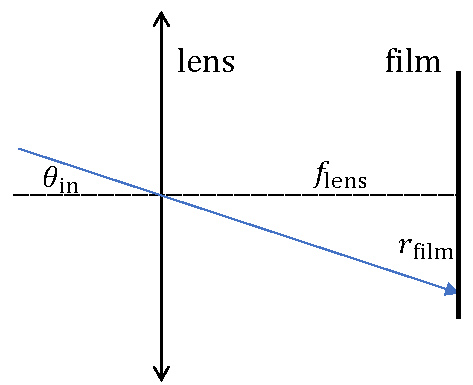
\includegraphics[width=0.5\linewidth]{img/pathfinder_sim_cam_pinhole.pdf}
    \caption{小孔成像的示意图。}
    \label{fig:pathfinder_sim_cam_pinhole}
\end{figure}

模拟得到的不同距离下灰度值在$r_\mathrm{film}$空间上的分布如图\ref{fig:pathfinder_sim_cam_gray_dist}所示,这里我们已经考虑了不同半径处所对应的环的大小(相空间大小)不同的效应。
我们可以看到在半径为0的附近存在一个明显的平台区,这对应的是发光球所形成的像,而在也有一部分随半径衰减的灰度区域,这是由经过散射的光子所形成的。

假设光源在方位角$\phi$方向是均匀的,那么我们可以通过模拟得到相机所拍摄的二维的照片,如图\ref{fig:pathfinder_sim_cam_img}所示。
在图中我们可以清晰地看到发光球在相机中所形成的像,以及像附近的光晕。

\begin{figure}[htb]
    \centering
    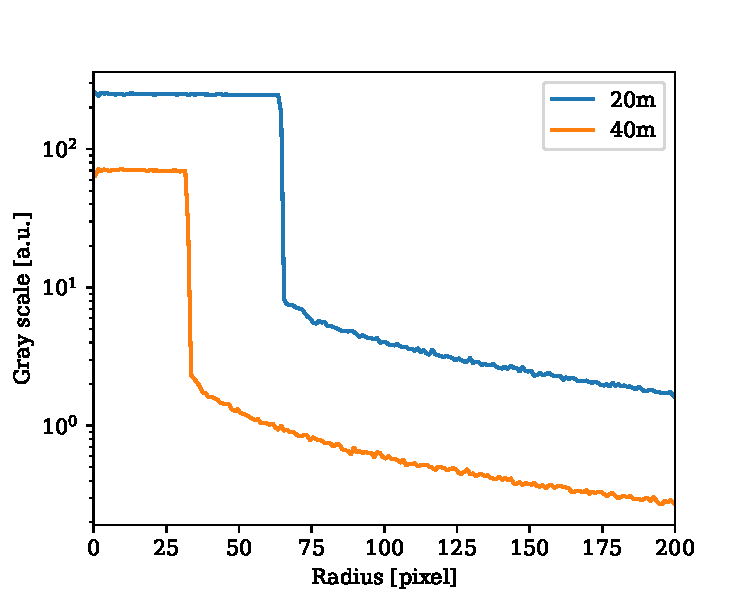
\includegraphics[width=0.75\linewidth]{img/pathfinder_sim_cam_gray_dist.pdf}
    \caption{模拟得到的相机灰度值在$r_\mathrm{film}$空间上的分布。}
    \label{fig:pathfinder_sim_cam_gray_dist}
\end{figure}

\begin{figure}[htb]
    \centering
    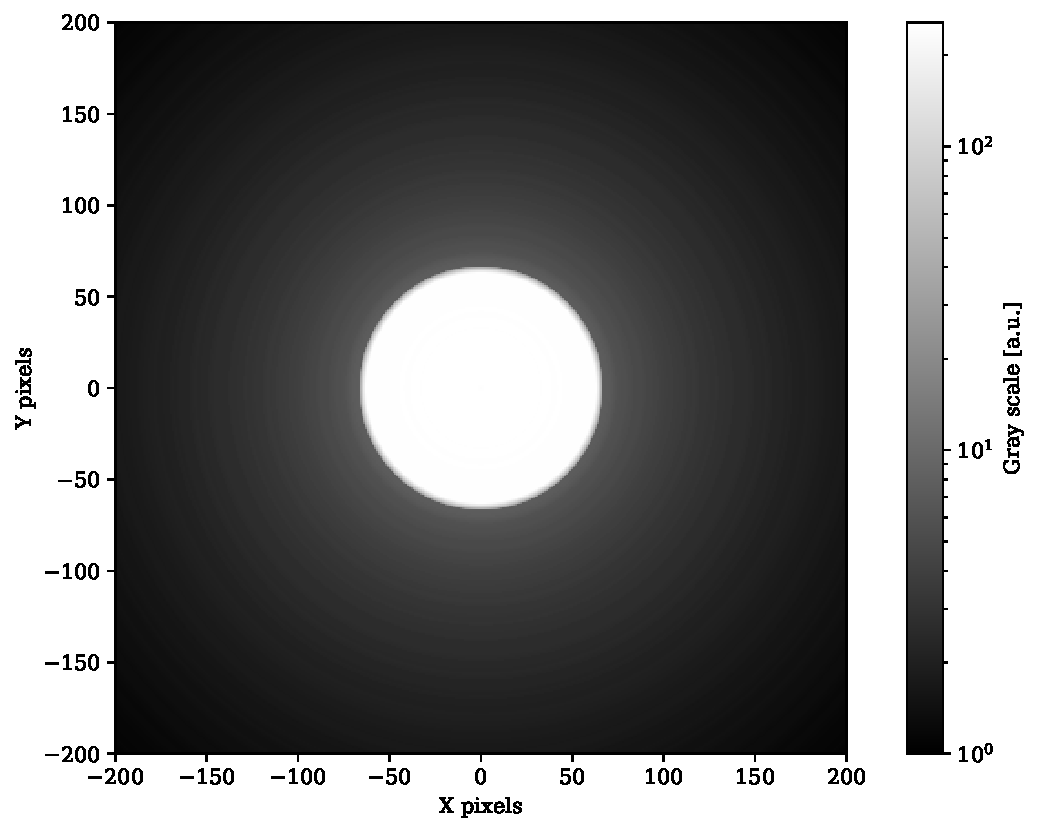
\includegraphics[width=0.75\linewidth]{img/pathfinder_sim_cam_img.pdf}
    \caption{模拟得到的相机在距离发光球$20\,\mathrm{m}$处拍摄得到的照片。为了更明显地看到相机的光晕,灰度值被以$\log$的形式显示成颜色。}
    \label{fig:pathfinder_sim_cam_img}
\end{figure}

PMT系统测量到的光子到达时间分布的模拟结果如图\ref{fig:pathfinder_sim_PMT_dist}所示。我们可以清晰地观察到经过散射之后的光子会到达得更晚一些,在到达时间分布图上形成一个拉长的散射尾巴。从这个散射尾巴的形状和高度中,我们可以分析出海水的散射性质\cite{OP_ANTARES:2004, OP_IceCube:2006, OP_IceCube:2013}。
这里,考虑到我们实验中的PMT在时间响应方面有大约$4\,\mathrm{ns}$的TTS,我们已经把模拟得到的精确的到达时间分布与一个半高宽为$4\,\mathrm{ns}$的高斯核做了卷积处理。

由于实验中的发光球内部结构相对复杂,球内的3D打印支架以及电子学的供电线和数据线会对光源有一定遮挡作用,因此实际情况中发光球的会存在一定的不均匀性\cite{pathfinder_light_source:2022}。
为考虑这种非各项均匀性对实验观测结果的影响,我们可以在模拟中计算光子在发射点的纬度位置所对应的$\theta_\mathrm{e}$:
\begin{equation}
    \theta_\mathrm{e} = \arccos \left( \frac{\vec{x}_\mathrm{r}}{\vert\vec{x}_\mathrm{r}\vert} \cdot \frac{\vec{x}_\mathrm{e}}{\vert\vec{x}_\mathrm{e}\vert}  \right) .
    \label{eq:latitude}
\end{equation}
通过对不同维度的光子增加或者减少权重的方式,来模拟发光球的不均匀性。

在图\ref{fig:pathfinder_sim_PMT_dist}中右侧子图中,我们把光子按照$\theta_\mathrm{e}$分成了多组,可以看到来自不同的维度的光子会形成不同的到达时间分布。
来自负的$\theta_\mathrm{e}$区域的光子只有在经过散射之后才能到达PMT,因此在几何预期到达时间上不存在峰,而拥有相对比较长的散射尾巴。

\begin{figure}[htp]
    \centering
    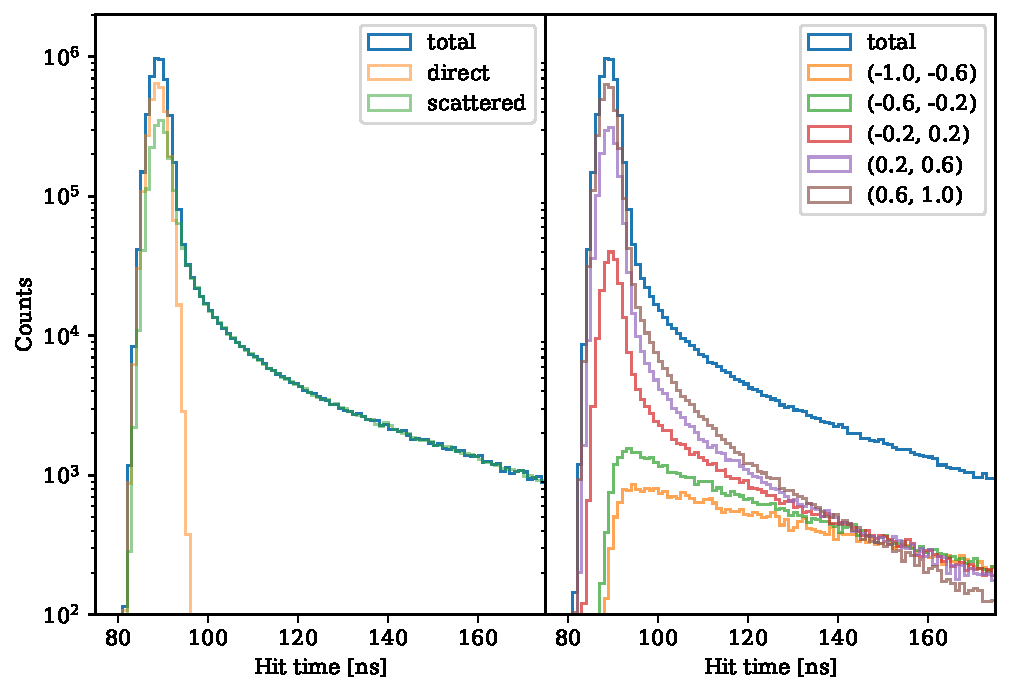
\includegraphics[width=1.0\linewidth]{img/pathfinder_sim_PMT_dist.pdf}
    \caption{在$20\,\mathrm{m}$处测得的光子到达时间分布。左图:光子被分成了散射和未被散射两组。右图:光子按照表示发射位置纬度的$\theta_\mathrm{e}$分成了多组。}
    \label{fig:pathfinder_sim_PMT_dist}
\end{figure}

\subsection{对分析方法进行研究和验证}
\label{sec:pathfinder_verification}

对于相机系统而言,我们主要关注相机视场中心的把相机摄到的照片的中心区域像素点的灰度值$I_\mathrm{center}$,即中心辐射度。
通过对比远近两处所拍摄到的照片的$I_\mathrm{center}$,可以海水的测量衰减长度$\lambda_\mathrm{att}$。这是因为相机有非常好的角分辨率,因此原本朝向相机前行的光子一旦发生散射,便有极大可能偏离原本目标的像素点。

在模拟中,我们可以对这一测量方法进行验证。我们按照表\ref{tab:pathfinder_sim_set}中的海水光学性质参数作为输入,并且改变发光球与接收球壳的距离,从$15\, \mathrm{m}$到$55\, \mathrm{m}$,其范围足以覆盖真实实验中的距离,进行多组不同的实验。
在模拟中,我们可以提取出中心像素区域所对应的光子,并且通过输出中记录的散射次数$k$来统计其中直接到达的光子的比例$\alpha$。如图\ref{fig:pathfinder_sim_cam_sca_ratio}所示,直接直接到达的光子的比例在不同距离下均保持很高的占比且非常稳定,$\alpha = 91 \pm 1 \%$。

\begin{figure}[htp]
    \centering
    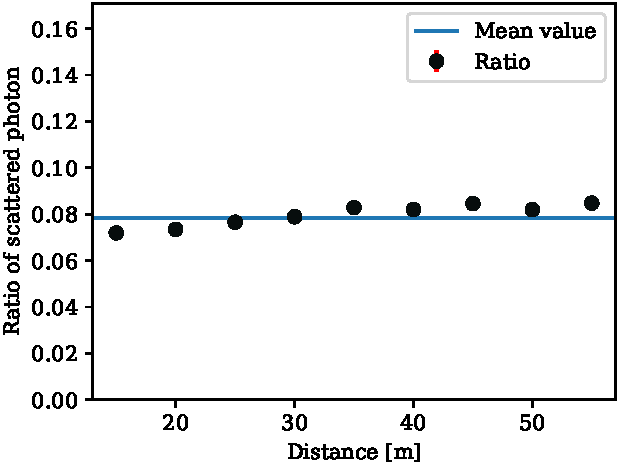
\includegraphics[width=0.65\linewidth]{img/pathfinder_sim_cam_sca_ratio.pdf}
    \caption{经过散射的光子在$I_\mathrm{center}$中所贡献的比例。}
    \label{fig:pathfinder_sim_cam_sca_ratio}
\end{figure}

根据比尔朗博定律\cite{Beer_Lambert_law:2020},我们可以通过测量$I_\mathrm{center}$中直接到达的光子数量随距离的衰减来测量衰减长度$\hat{\lambda}_\mathrm{att}$:
\begin{equation}
    I_{\mathrm{center}}(d) \propto \frac{1}{\alpha} \exp(-\frac{d}{\hat{\lambda}_\mathrm{att}}) , 
    \label{eq:pathfinder_cam_Icenter_def}
\end{equation}

在模拟中我们可以对这种测量方法进行检验,如图\ref{fig:pathfinder_sim_cam_Icenter_fit}所示。
对不同距离下的$I_{\mathrm{center}}$很好地满足了公式\ref{eq:pathfinder_cam_Icenter_def}所描述的关系,其拟合结果为$\hat{\lambda}_\mathrm{att} = 18.13 \pm 0.18 \,\mathrm{m}$。
这与我们在模拟中输入的值$\lambda_\mathrm{att} = 17.75 \,\mathrm{m}$相差仅为$2\%$,在实验预期的精度范围之内。
存在这种误差的原因是,直接到达的光子的比例$\alpha$实际上会随着距离的增加而轻微地衰减。
如果我们在对模拟数据的计算中考虑到$\alpha$衰减的影响的话\footnote{注意,在实际时间数据中并不能采用这样操作,因为我们无法区分经过散射的光和直接到达的光},那么可以得到$\hat{\lambda}_\mathrm{att} = 17.85 \pm 0.10 \,\mathrm{m}$,完美地验证了比尔朗博定律。

\begin{figure}[htp]
    \centering
    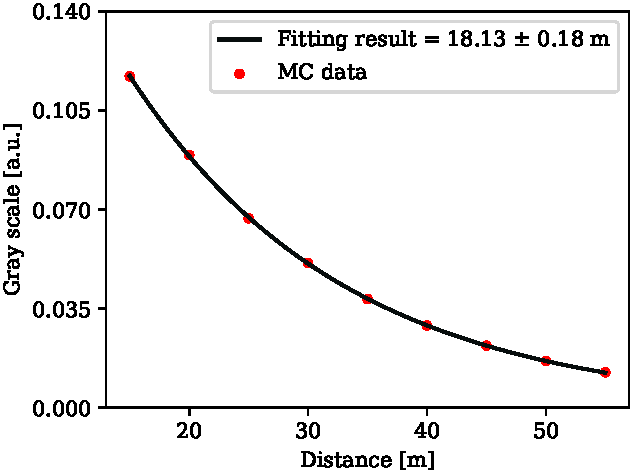
\includegraphics[width=0.6\textwidth]{img/pathfinder_sim_cam_Icenter_fit.pdf}
    \caption{中心像素点的灰度值$I_{\mathrm{center}}$随距离的变化以及拟合结果。}
    \label{fig:pathfinder_sim_cam_Icenter_fit}
\end{figure}

PMT系统也可以通过对比远近两处测得的光子数来预测海水的衰减长度。
在过去实验\cite{OP_ANTARES:2004, OP_P-One:2021}中的一种常见做法是通过PMT探测到的总光子数之比来估计衰减长度:
\begin{equation}
    \hat{\lambda}_\mathrm{att,eff}^\mathrm{tot} = (d_1 - d_2) / \ln \left( \frac{N_\mathrm{2}^\mathrm{tot} d_2^2}{N_\mathrm{1}^\mathrm{tot} d_1^2} \right) ,
    \label{eq:pathfinder_PMT_att_eff}
\end{equation}
其中$N_1^\mathrm{tot}$和$N_2^\mathrm{tot}$分别表示位于$20\,\mathrm{m}$和$40\,\mathrm{m}$处的PMT所测到的总光子数。

然而我们的模拟研究表明,用这种方法测量得到的$\hat{\lambda} _\mathrm{att,eff} ^\mathrm{tot}$并不能估计真正的$\lambda _\mathrm{att}$。
如图\ref{fig:pathfinder_sim_PMT_att}所示,我们进行了不同批次的数值模拟,在控制其他光学性质参数相同的情况下将瑞利散射的长度从$100\,\mathrm{m}$调整到了$300\,\mathrm{m}$,来观察两种散射长度的变化。
我们发现$\hat{\lambda} _\mathrm{att,eff} ^\mathrm{tot}$相比于$\lambda _\mathrm{att}$可以大出$\sim 40\%$的值。
这是因为PMT的视场范围比较大,接收的总光子中包含了大量的经过散射的光子,且散射的光子数所占的比例随距离变化明显,如图\ref{fig:pathfinder_sim_PMT_sca_ratio}所示。

另一种可以用于估计衰减长度的计算方法是将公式\ref{eq:pathfinder_PMT_att_eff}中的$N^\mathrm{tot}$替换为$N^\mathrm{peak}$,即只选取光子到达时间分布峰值前后$3 \times \mathrm{TTS}$的时间窗口内的光子。
用这种方式估计出来的衰减长度记为$\hat{\lambda} _\mathrm{att,eff} ^\mathrm{peak}$,如图\ref{fig:pathfinder_sim_PMT_att}中所示,我们可以发现$\hat{\lambda} _\mathrm{att,eff} ^\mathrm{peak}$与$\lambda _\mathrm{att,avg}$(公式\ref{eq:pathfinder_att_avg})的值相接近,误差在$3\%$以内。
这是因为对于PMT所观测到的峰值附近的光子而言,它们通常要么没有被散射,要么只发生了前向散射,因此它们的数量可以用于估计$\lambda _\mathrm{att,avg}$。

\begin{figure}[!ht]
    \centering
    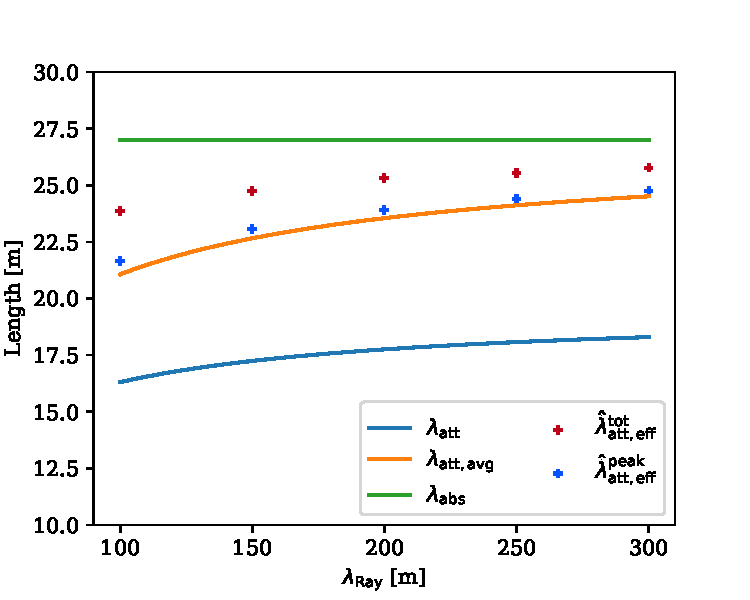
\includegraphics[width=0.8\linewidth]{img/pathfinder_sim_PMT_att.pdf}
    \caption{不同方式计算得到的吸收长度与真实模拟输入量之间的对比。}
    \label{fig:pathfinder_sim_PMT_att}
\end{figure}


除了估计$\lambda _\mathrm{att,avg}$以外,PMT系统还能用如下的方式来测量$\lambda _\mathrm{abs}$:
\begin{equation}
    \int_{-\infty}^{\infty} \mathcal{N}_1(t) e^{\frac{c t}{n_\mathrm{g} \lambda_\mathrm{abs}}} ~\mathrm{d}t \times d_1^2 = 
    \int_{-\infty}^{\infty} \mathcal{N}_2(t) e^{\frac{c t}{n_\mathrm{g} \lambda_\mathrm{abs}}} ~\mathrm{d}t \times d_2^2 ,
    \label{eq:pathfinder_PMT_abs}
\end{equation}
其中$\mathcal{N}(t) = \frac{\mathrm{d}N}{\mathrm{d}t}$是光子到达时间分布,$n_\mathrm{g}$是介质的群速度折射率,$c$表示光速。
这种测量方式利用了PMT系统能够记录光子到达时间的特性,它将PMT测量的时间信息转换成了光子传播的径迹长度$l = c t / n_\mathrm{g}$。
而径迹长度又可以被转换为光子没有被吸收的概率,因此我们有光子成功到达探测器的概率为:
\begin{equation}
    e^{\frac{c t}{n_\mathrm{g} \lambda_\mathrm{abs}}} ,
\end{equation}
这一概率项在公式\ref{eq:pathfinder_PMT_abs}中可以视作光子加合时的权重项。

公式\ref{eq:pathfinder_PMT_abs}的一个优秀性质是它能够在对到达时间分布做卷积变换后依然保持成立。
由于实验过程中PMT存在TTS,LED光源也存在有限的脉冲宽度,因此我们实际上观测到的光子到达时间分布$N_\mathrm{obs}(t)$会被弥散掉。
我们假设对于远近两支PMT的弥散核函数$G(\tau)$是相同的,那么我们可以证明对于公式\ref{eq:pathfinder_PMT_abs}的一边来说,卷积前后只会相差一个$\mathcal{G} = \int_{-\infty}^{\infty} G(\tau) e^{\frac{c\tau}{n_\mathrm{g} \lambda_\mathrm{abs}}} ~\mathrm{d}\tau$的因子,如公式\ref{eq:pathfinder_PMT_abs_conv}中所示。
而这个因子只和卷积核的函数形式与介质中的吸收长度有关,因此对于远近两支PMT而言是相同的。故公式\ref{eq:pathfinder_PMT_abs}中的关系在经过卷积后依然能保持成立。

\begin{equation}
    \begin{aligned}
    & ~~~\int_{-\infty}^{\infty} \mathcal{N}_\mathrm{obs}(t) e^{\frac{ct}{n_\mathrm{g} \lambda_\mathrm{abs}}} ~\mathrm{d}t \\
    &= \int_{-\infty}^{\infty} G(\tau) \mathcal{N}(t-\tau) e^{\frac{ct}{n_\mathrm{g} \lambda_\mathrm{abs}}} ~\mathrm{d}t \mathrm{d}\tau \\
    &= \int_{-\infty}^{\infty} G(\tau) e^{\frac{c\tau}{n\lambda_\mathrm{abs}}} ~\mathrm{d}\tau \times
    \int_{-\infty}^{\infty} \mathcal{N}(t-\tau) e^{\frac{c(t-\tau)}{n_\mathrm{g} \lambda_\mathrm{abs}}} ~\mathrm{d}t \\
    &= \mathcal{G} \int_{-\infty}^{\infty} \mathcal{N}(t) e^{\frac{ct}{n_\mathrm{g} \lambda_\mathrm{abs}}} ~\mathrm{d}t
    \label{eq:pathfinder_PMT_abs_conv}
    \end{aligned}
\end{equation}

\begin{figure}[!ht]
    \centering
    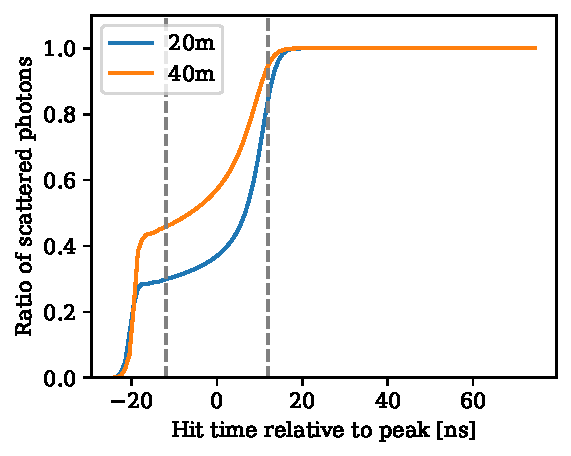
\includegraphics[width=0.65\linewidth]{img/pathfinder_sim_PMT_sca_ratio.pdf}
    \caption{不同时间段内,PMT测到的光子中散射光子所占的比例。}
    \label{fig:pathfinder_sim_PMT_sca_ratio}
\end{figure}


\section{PMT系统的测试}

PMT是本次海铃探路者实验中的两大系统之一,也是未来海铃中微子望远镜阵列中最核心的光敏元件。对PMT的详细研究和测试有助于我们深入地理解PMT的原理和过程,了解测量的精度和潜在的误差,是各个使用PMT的实验中都必不可少的环节\cite{KM3NeT_PMT:2018, IceCube_PMT:2019, JUNO_PMT:2022}。

\subsection{PMT的筛选}

\begin{figure}[ht]
    \centering
    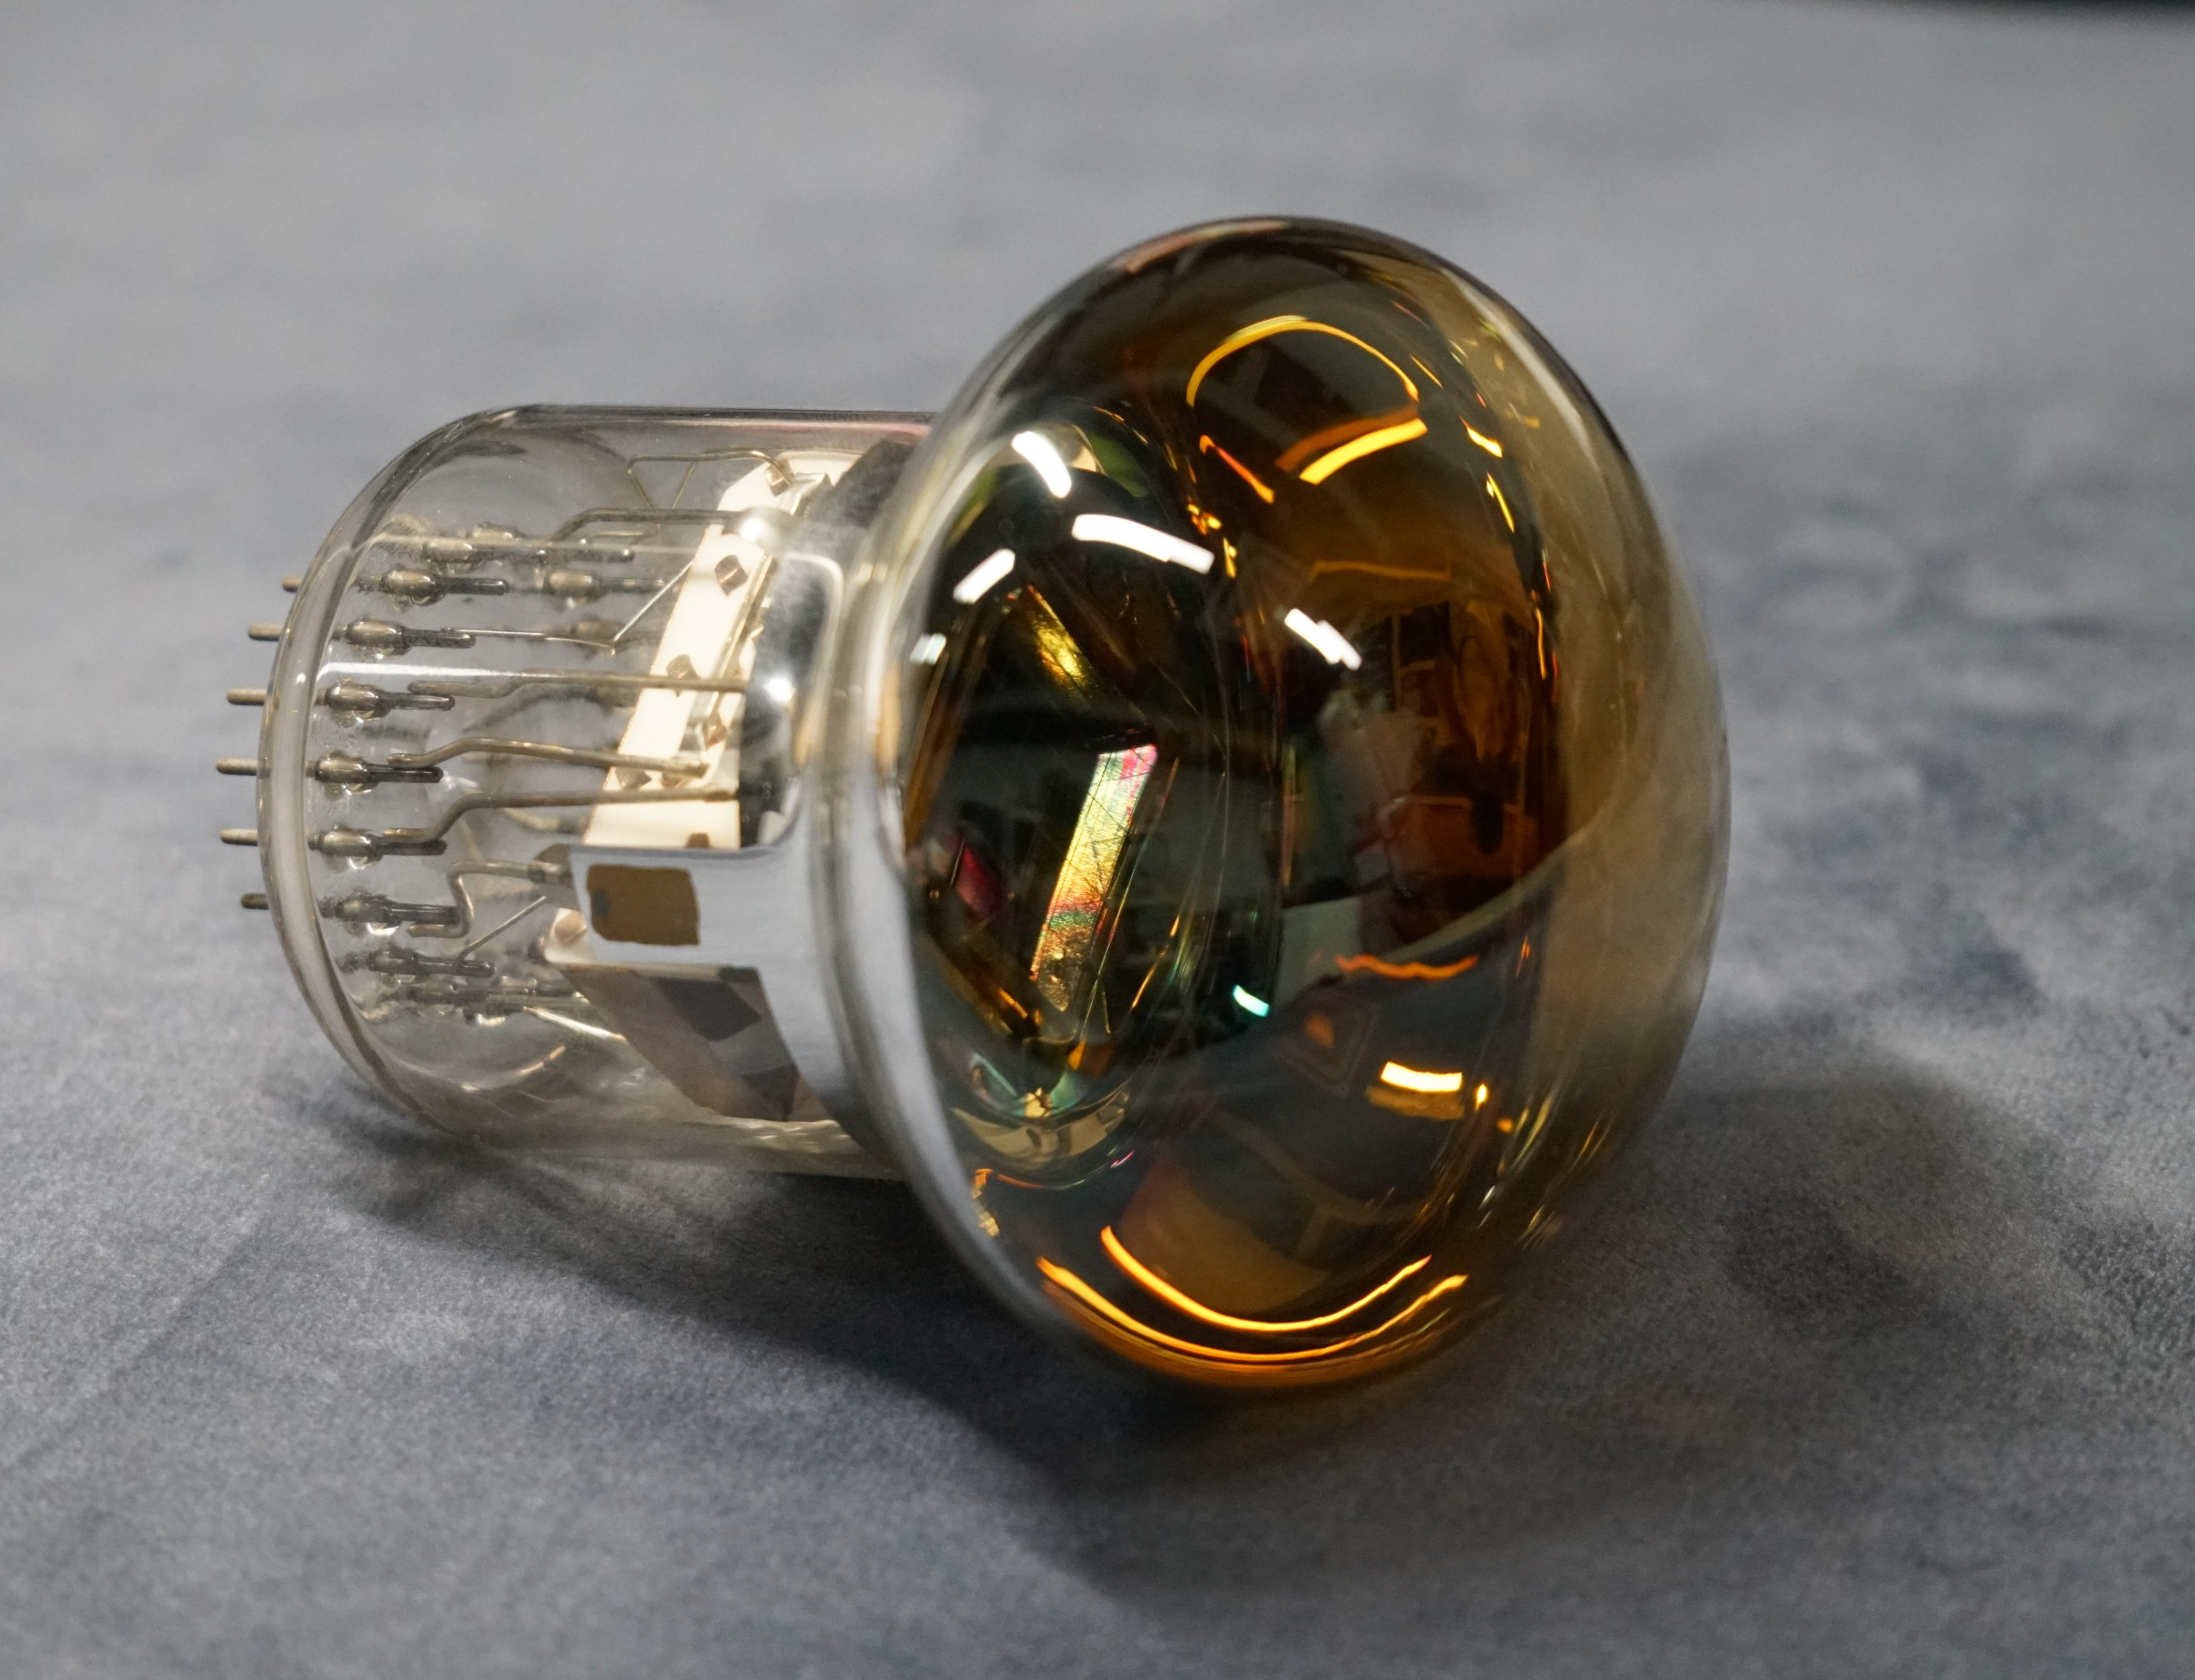
\includegraphics[width=0.5\textwidth]{img/pmt_image.jpg}
    \caption{在探路者实验中使用的HZC-XP72B22型号的PMT。}
    \label{fig:pmt_view}
\end{figure}

在我们选择海南展创光子技术有限公司(HZC)生产的XP72B22型号的PMT用于海铃探路者实验。该PMT的图片和特性分别在图\ref{fig:pmt_view}和表\ref{tab:pmt_properties}中显示。这种类型的PMT也被JUNO使用,并且是3英寸XP72B20 PMT的升级版本,具有优化的玻璃球形状以提高光收集效率和传输时间展宽\cite{JUNO_PMT:2021}。

\begin{table}[ht]
    \centering
    \caption{HZC-XP72B22型PMT的典型特征}
    \begin{tabular}{c|c}
        \hline
        玻璃材料 & 低钾含量的硼硅酸盐玻璃 \\
        \hline 
        光阴极材料 & Bi-alkali \\
        \hline
        $420\,\mathrm{nm}$下折射率 & 1.54 \\
        % \hline
        %  Supply Voltage & 1500V, max \\ 
         \hline
         典型高压值 & 1150 V \\
         \hline
         典型增益 & $6\times 10^3$ \\
         \hline
         暗噪声率 & 小于2 kHz \\ 
         \hline
         $404\,\mathrm{nm}$下的量子效率 & 28$\%$ \\
         \hline
         $470\,\mathrm{nm}$下的量子效率 & 20$\%$ \\
         \hline 
    \end{tabular}
    \label{tab:pmt_properties}
\end{table}

\begin{figure}[!htb]
    \centering
    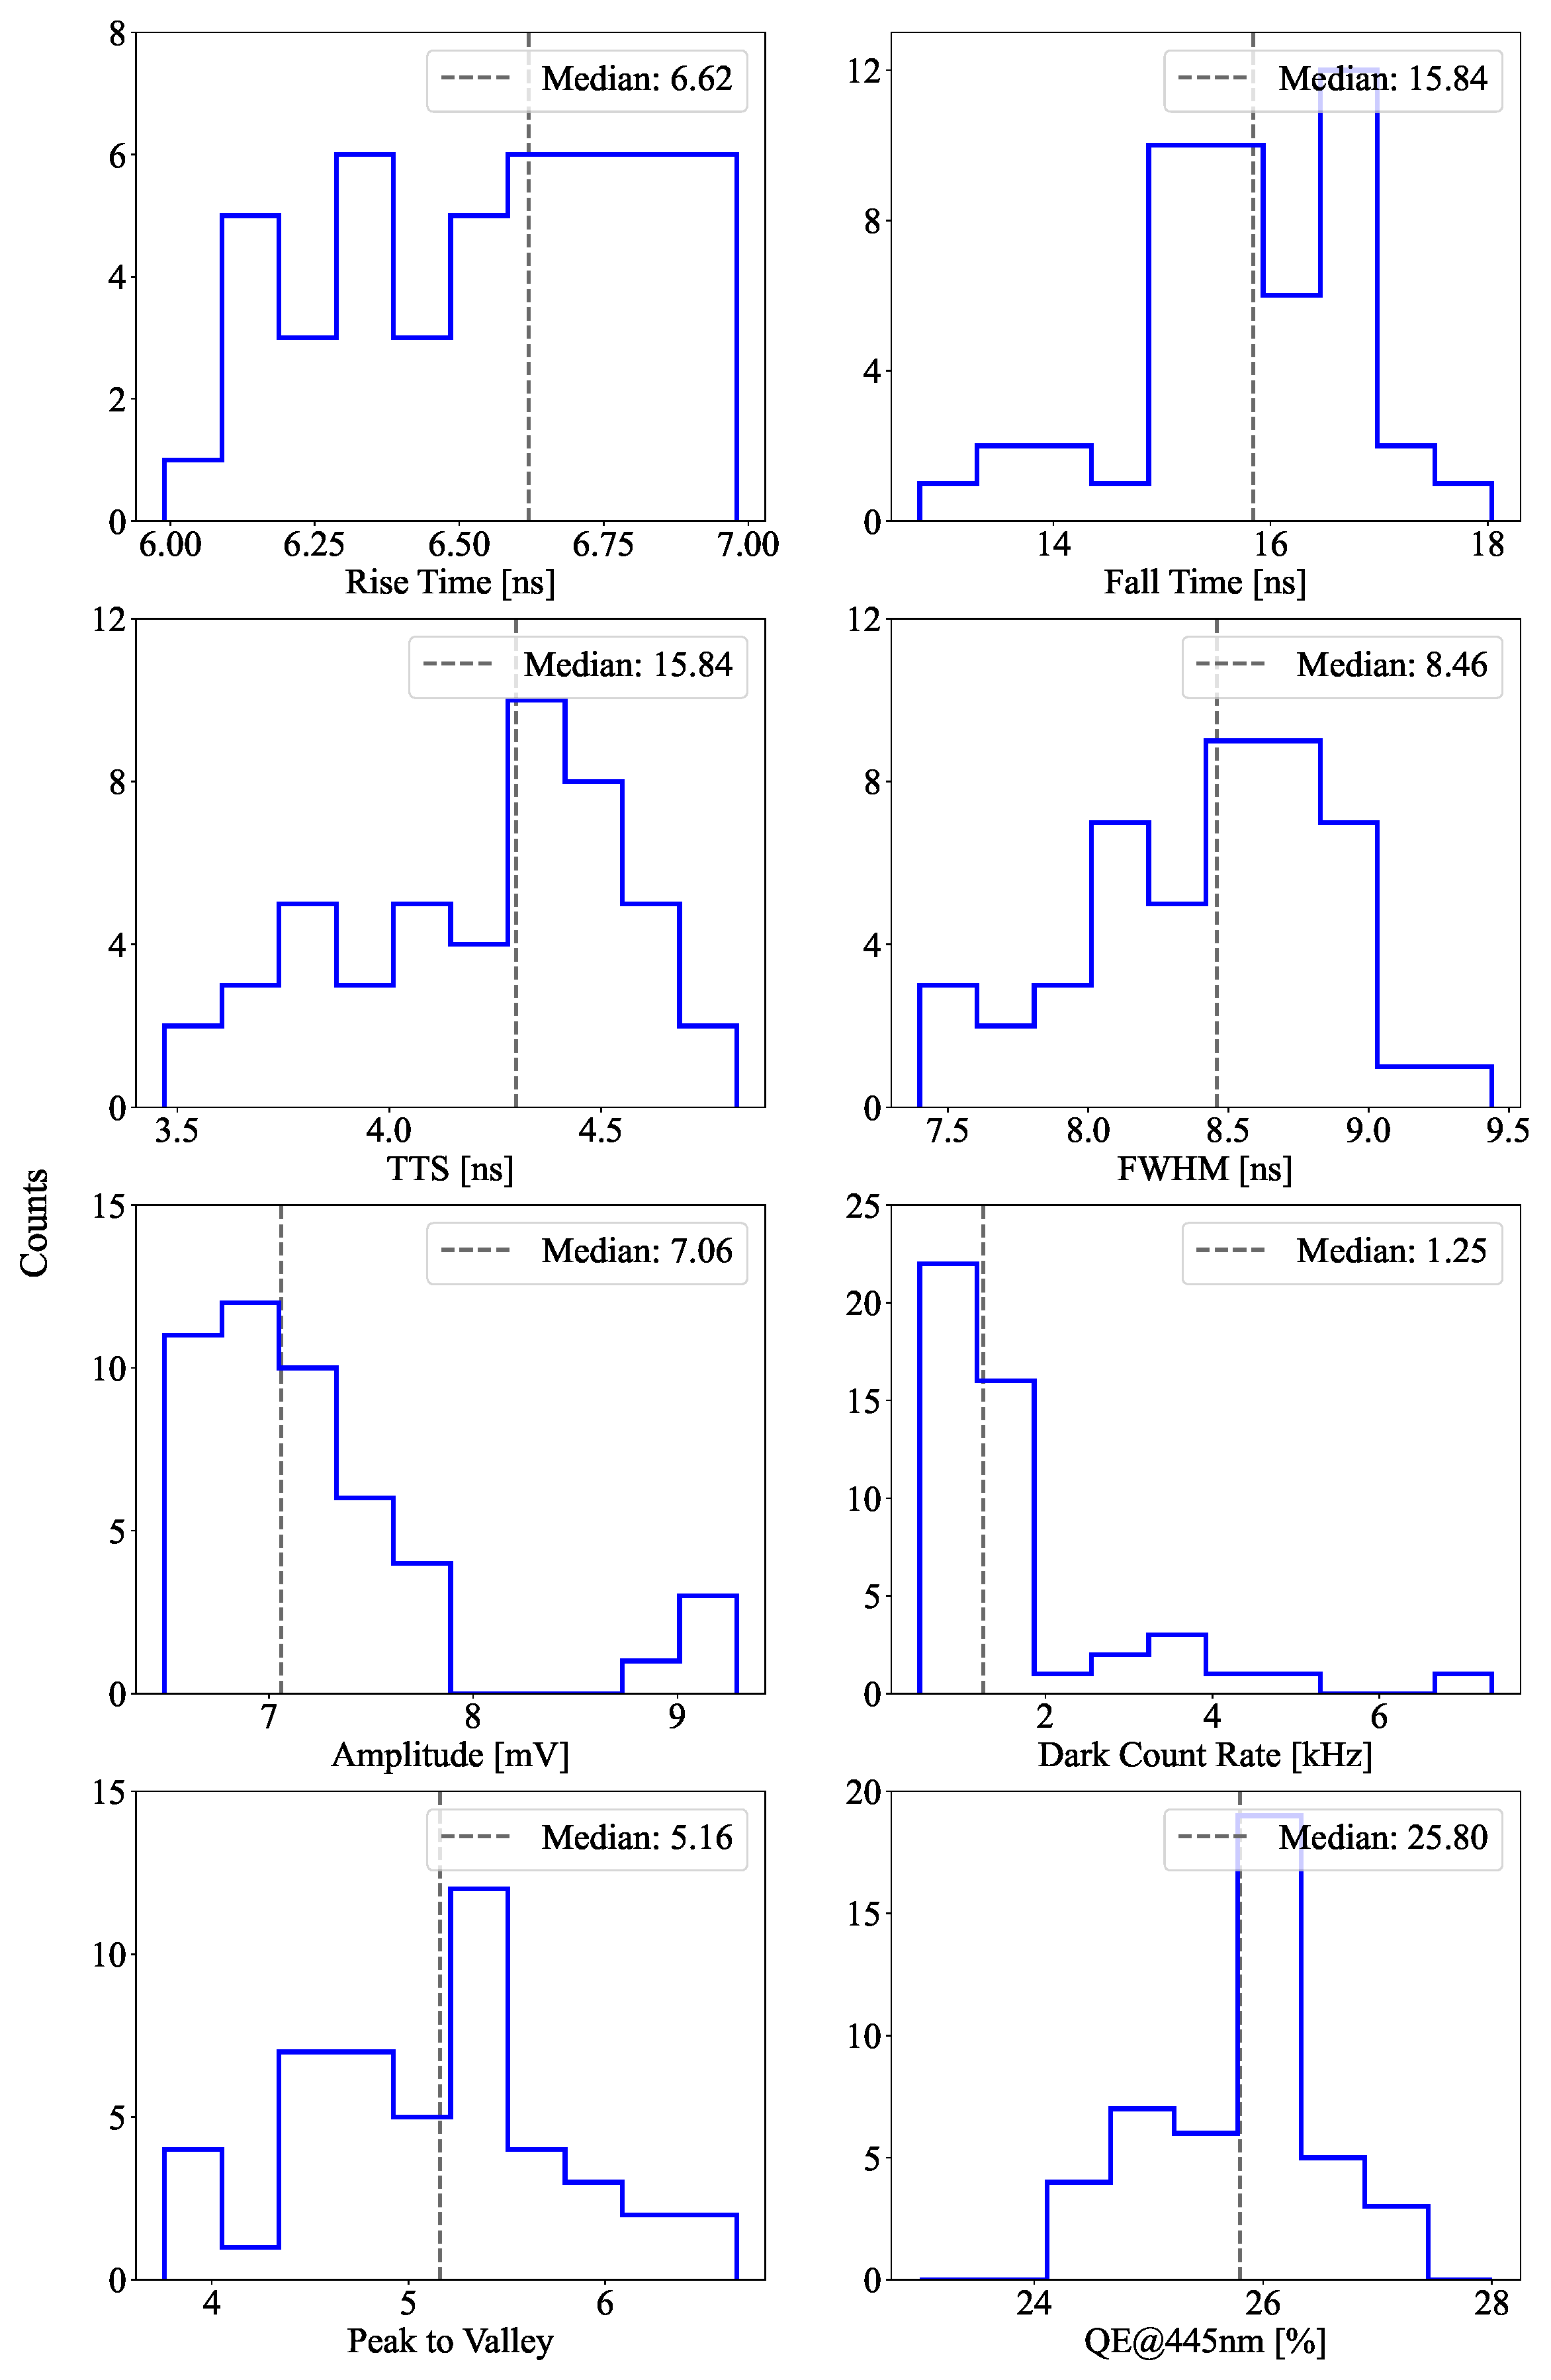
\includegraphics[width=0.85\textwidth, height=195mm]{img/pmt_ustc_test_result.pdf}
    \caption{在增益为$10^7$下,50支PMT的各种性质的测量结果分布,其中虚线表示中位数。}
    \label{fig:ustc_pmt}
\end{figure}

我们使用了一套中国科技大学的曾今为LHAASO的PMT进行批量测试的平台\cite{PMT_test:2020},来对我们购买的50支PMT样本进行了单独测试,并从中挑选出6支最合适的PMT来安装在两个接收球中。
在测试平台中,每一只PMT都被放置在独立的暗箱中,并通过一根光纤与一台皮秒激光器相连接。
整套测试系统由LabView程序控制,它会先对加载在PMT上的高压从$1100,\text{V}$到$1500,\text{V}$进行一轮扫描,来确定PMT的增益随电压变化的关系曲线。
然后通过调整天涯使得PMT在从$2\times10^6$到$1\times10^7$的增益范围内,每隔$10^6$的增益就测量一次PMT的性能。其测量的性质包括上升时间、下降时间、传输时间展宽(TTS)、单光电子(PE)电压、暗计数率(DCR)、峰谷比以及量子效率(QE)。
在增益为$10^7$下,50支PMT的性质测量结果被总结在图 \ref{fig:ustc_pmt} 中。
其中,对选取探路者下海使用的PMT而言最重要的三个性质和其中位数分别是:量子效率:$\sim25.8\%$,暗计数率:$\sim1.25~\text{kHz}$,TTS:$4.3~\text{ns}$。

在探路者实验时,我们需要在科考船的甲板上将实验装置布放到水下,因此甲板布放过程中PMT难免会暴露在光照下,这会影响PMT的阴极材料,使PMT在短期内的暗噪声率升高。
我们的实验装置从水面缓慢下降到海底所需要的时间约为一小时,在这一小时内PMT的暗噪声率会逐渐降低。
我们在实验室中测量了PMT的暗噪声率冷却所需要的时间。我们首先把PMT暴露在照度为$15~\text{lux}$的光下$15~\text{分钟}$,然后在PMT两端加上$1375~\text{V}$的电压并测量其暗噪声率率随时间的变化曲线。
典型的暗噪声率冷却曲线如图\ref{fig:exposure_time}所示,我们可以看到PMT需要约$60~\text{分钟}$才能恢复到低而稳定的暗噪声速率。

基于对探路者实验的要求以及以上的实验室测试结果,我们最终选取的六个PMT具有以下的性质:QE在$445~\text{nm}$处$>24\%$,TTS $<4~\text{ns}$,标准状态下DCR$<1.5~\text{kHz}$,在光照后1小时内DCR能恢复到$<2~\text{kHz}$的水平。

\begin{figure}[htb]
    \centering
    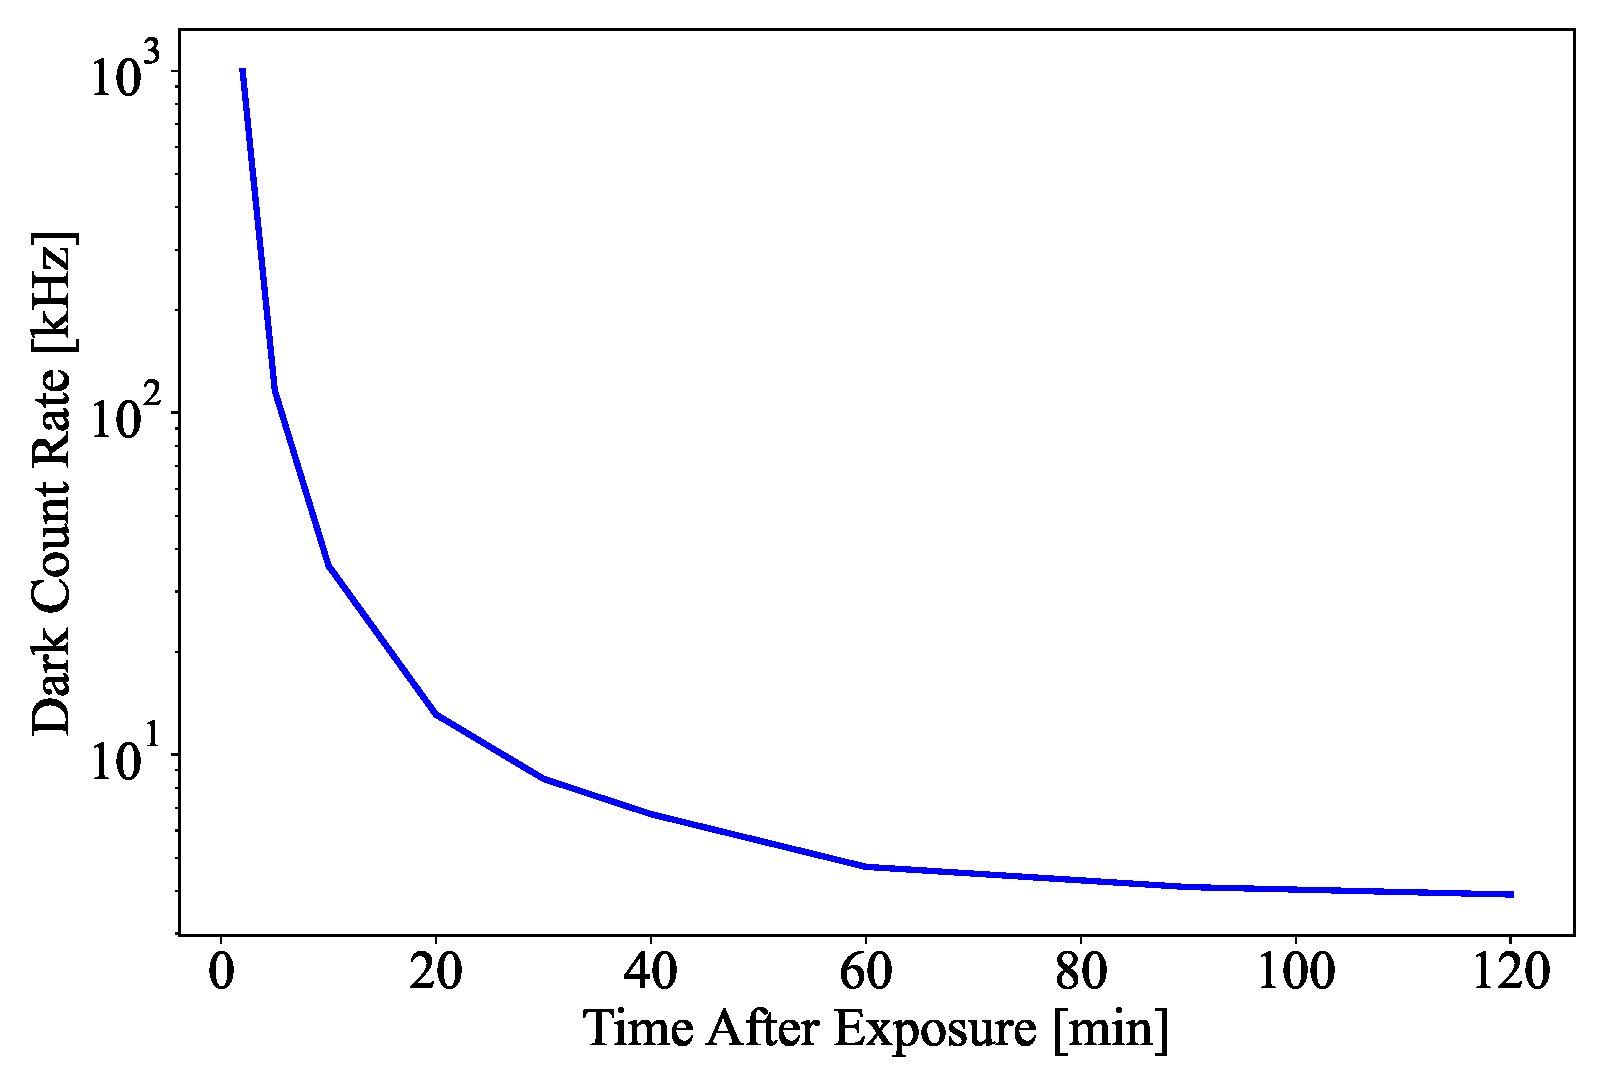
\includegraphics[width=0.70\textwidth]{img/pmt_dcr_after_exposure.pdf}
    \caption{在经过15分钟的曝光之后,PMT的暗噪声率随时间的变化。}
    \label{fig:exposure_time} 
\end{figure}

\subsection{PMT系统的低温刻度实验}

\begin{figure}[ht] 
    \centering
    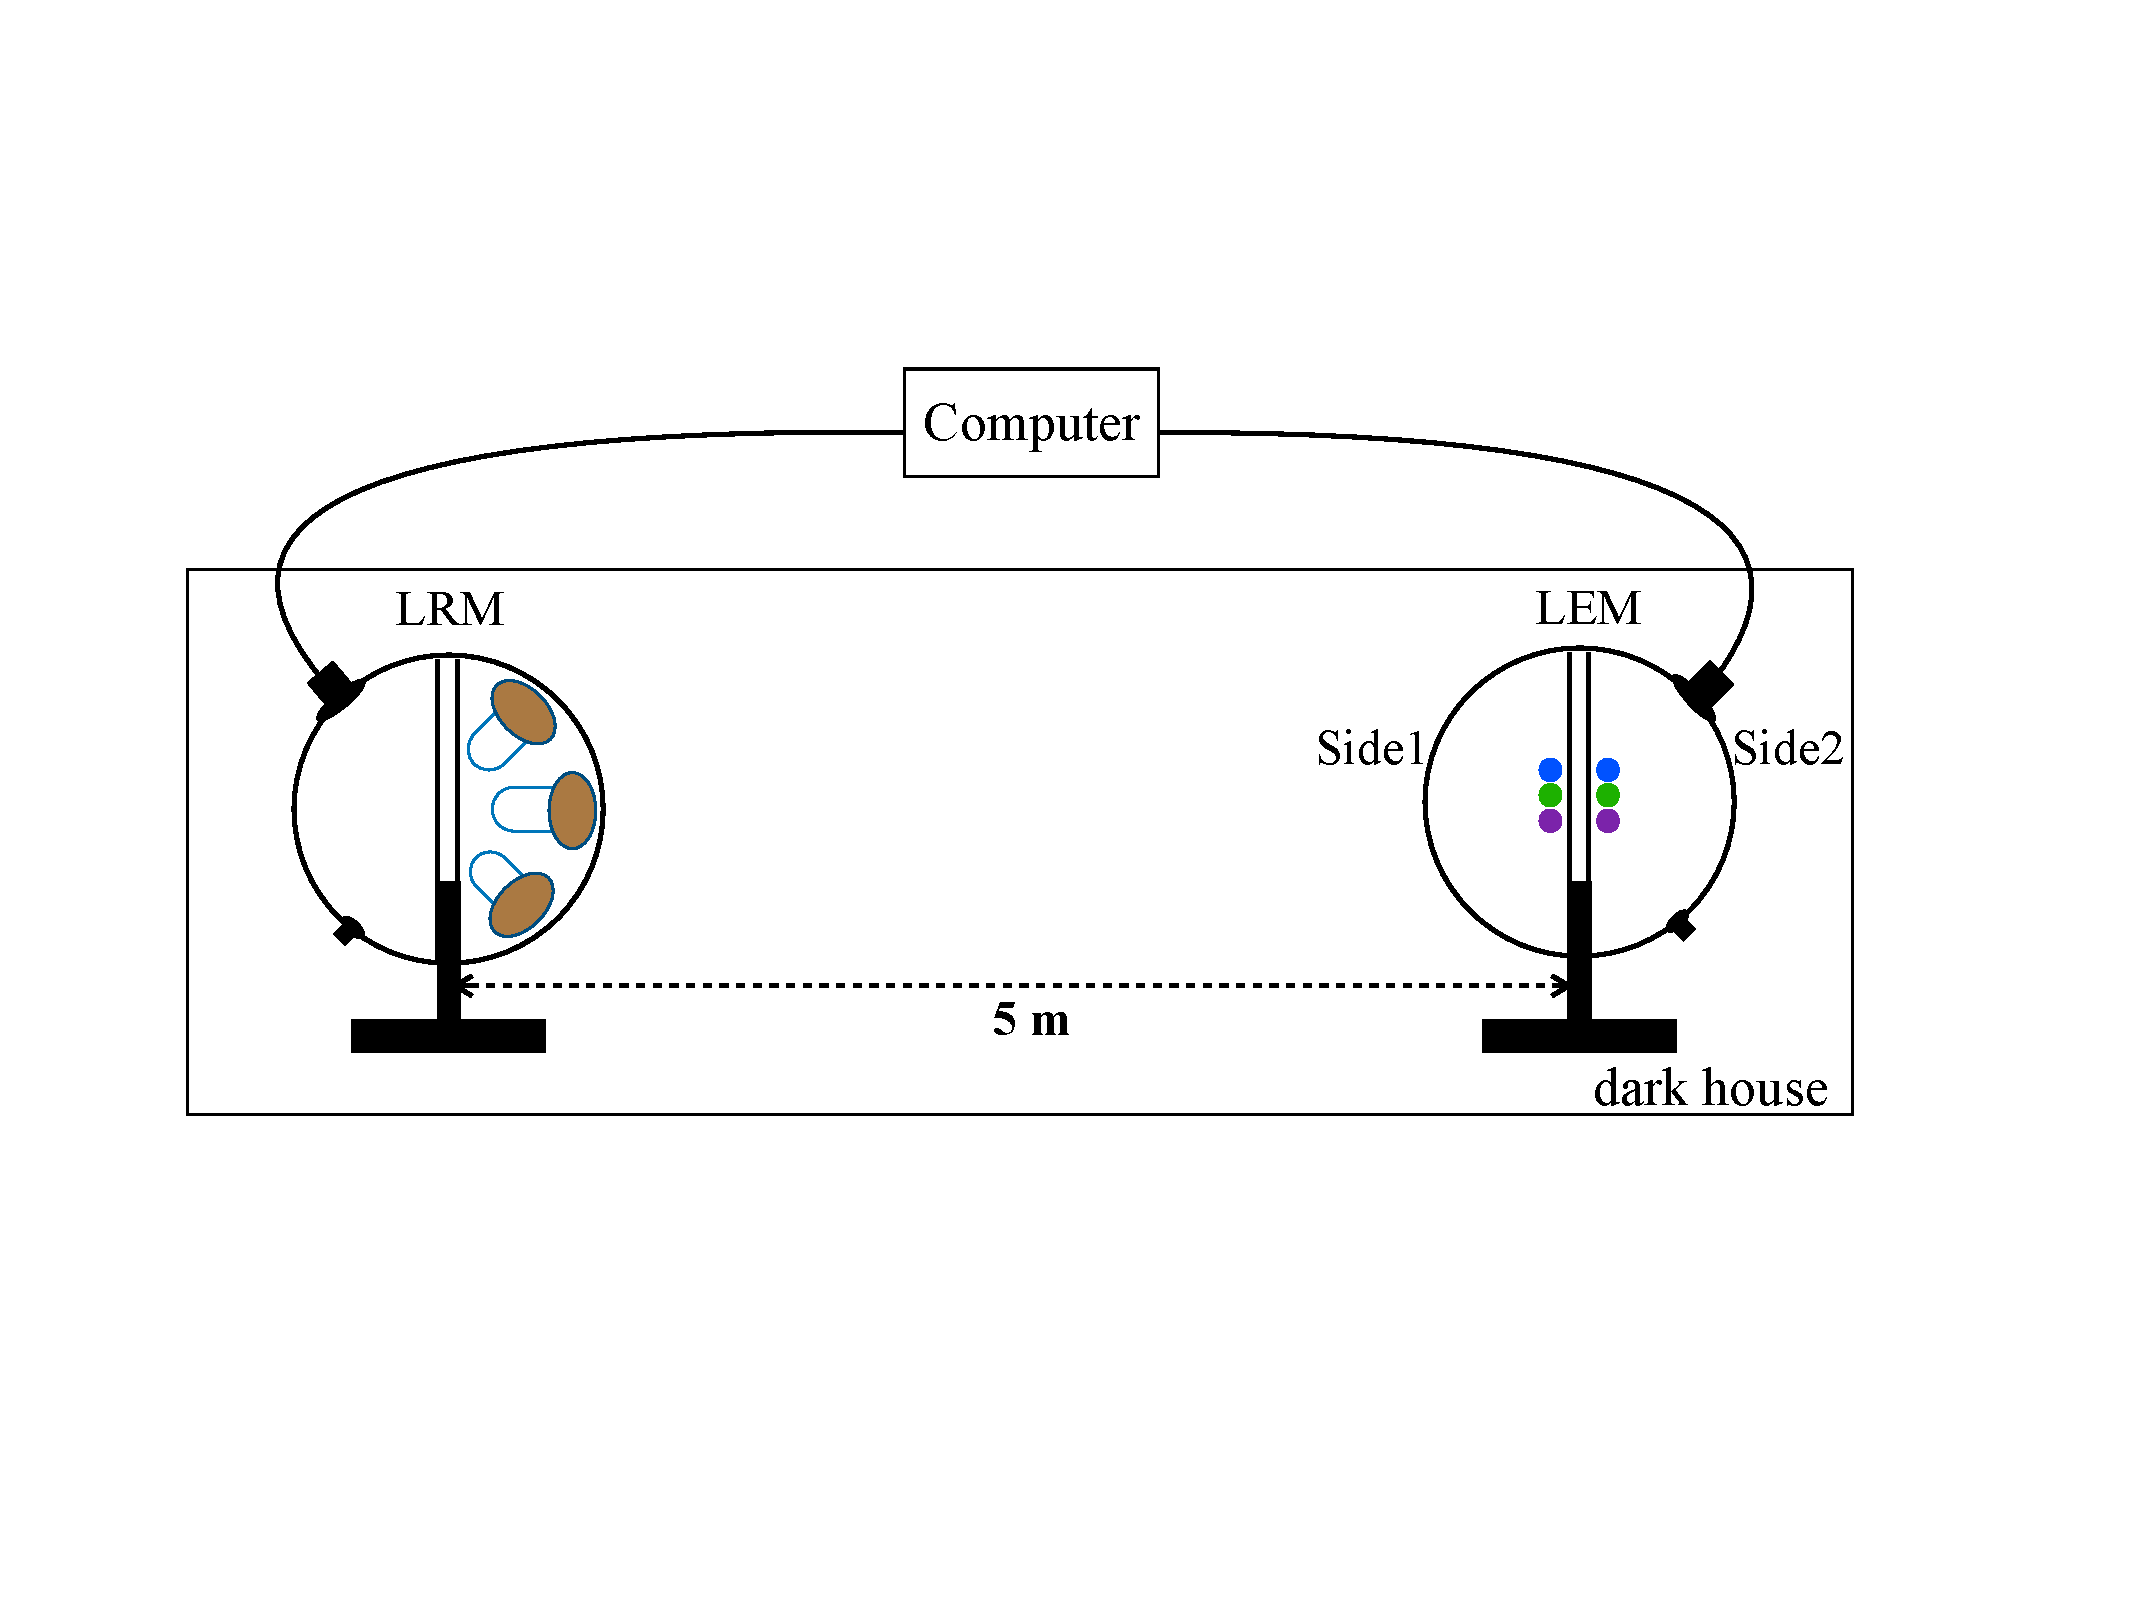
\includegraphics[width=0.92\textwidth]{img/pmt_cold_test_setup.pdf}
    \caption{低温刻度实验的配置示意图。}
    \label{fig:pmt_cold_test_setup}
\end{figure}

深海水的温度约为2摄氏度,而温度环境对PMT和LED的表现有所影响。
我们需要研究发光球和接收球在相同温度下的表现,特别是相对PMT探测效率、LED发射和时间特性。因为这些因素对我们解析探路者的数据,研究深海海水的光学性质有直接的影响。

刻度实验在一个体积约为$2\,\text{m} \times 2\,\text{m} \times 7\,\text{m}$的能自由控制温度暗室中进行。刻度的设置如图\ref{fig:pmt_cold_test_setup}所示。
在暗室中,单个发光球和接收球之间形成一个共同的水平轴,它们的距离被固定在$5\,\text{m}$。
为了测量发光球两个半球的亮度比,发光球的每个半球分别作为独立的光源,分别标记为A面和B面。同时,为了测量PMT的相对探测效率,在刻度实验中,两个接收球轮流充当光接收器,并接收发光球的每一侧发射的光。
在远端和近端接收球中,六个PMT被标记为1、2、3和4、5、6的ID号。
总共设置了四种不同的接收器和发射器组合,编号为1、2、3、4,详见表\ref{tab:pmt_low_temp_exp_config}。其中,编号1和4是探路者实验中实际使用的组合。
为了抵消接收球中三个PMT方向的残留非对称效应,在每个组的测量中,通过沿着它们的中心轴旋转接收球三个不同的角度(0、120、240)来重复三次测量。
共进行了12次刻度实验,下文中呈现的结果是在不同旋转角度下进行测量的平均值。

\begin{table}[htb]
    \centering
    \begin{tabular}{|c|c|c|c|}
        \hline
        编号(GroupID) & 发光球 & 接收球 & PMT IDs\\
        \hline                            
        1  & A面 & far 接收球 & 1,2,3       \\
        2  & B面 & far 接收球 & 1,2,3   \\
        3  & A面 & near 接收球 & 4,5,6     \\
        4  & B面 & near 接收球 & 4,5,6    \\
        \hline
    \end{tabular}
    \caption{刻度实验中的测量组。发光球的两个半球分别标记为A面和B面,作为刻度实验中独立的光源。两个接收球被标记为近端和远端,以表示它们在探路者实验中的距离。编号1和4是探路者实验中使用的组合。}
    \label{tab:pmt_low_temp_exp_config}
\end{table}

在刻度实验中,DAQ的配置与探路者实验实际实验中相同:在每个接收球中,三个PMT和发光球中的脉冲LED均以外部触发的方式触发,触发率为$10~\mathrm{kHz}$;PMT信号由$250~\mathrm{MHz}$的ADC数字化,结果得到$1000~\mathrm{ns}$的DAQ窗口。
图\ref{fig:pmt_spe_waveform}显示了PMT波形的一个示例,其中ADC值的波动是由电子噪声引起的,每个ADC点表示约$0.43~\mathrm{mV}$。

\begin{figure}[htb]
    \centering
    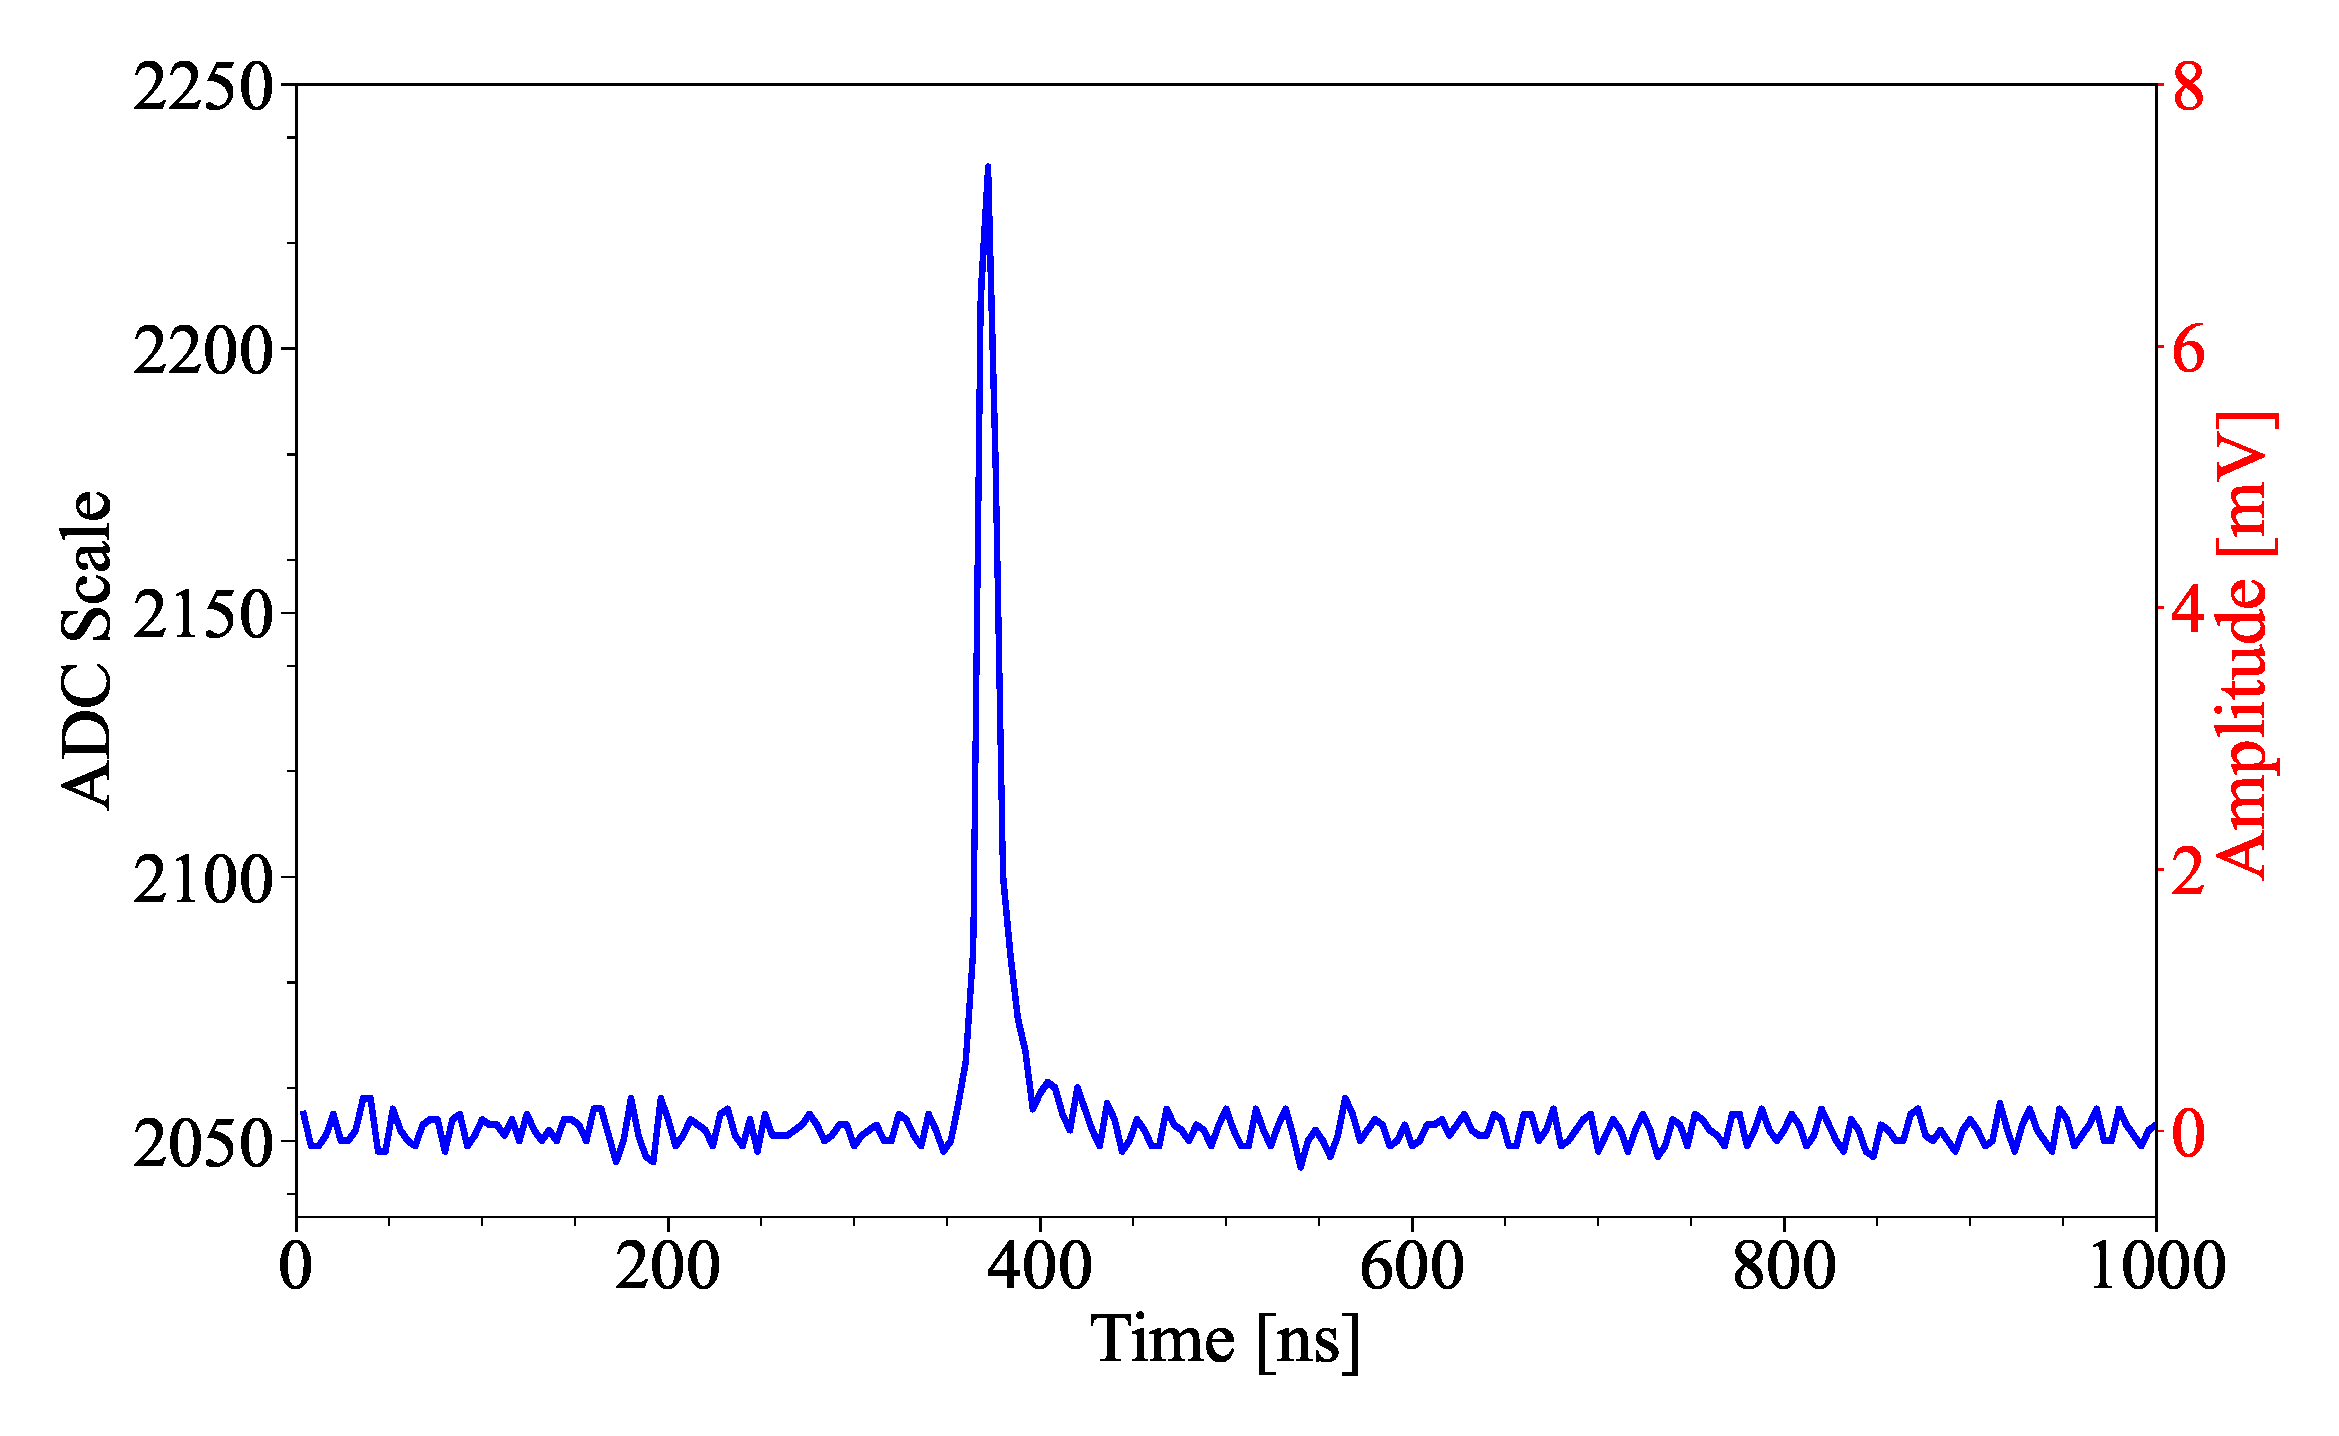
\includegraphics[width= 0.82\textwidth]{img/pmt_spe_waveform.pdf}
    \caption{DAQ采集得到的一个典型的单光子波形。其中右侧的y轴表示波形对应的电压值。}
    \label{fig:pmt_spe_waveform}
\end{figure}

\subsubsection{光电子的峰值高度与增益测试}

\begin{figure}[!ht]
    \centering
    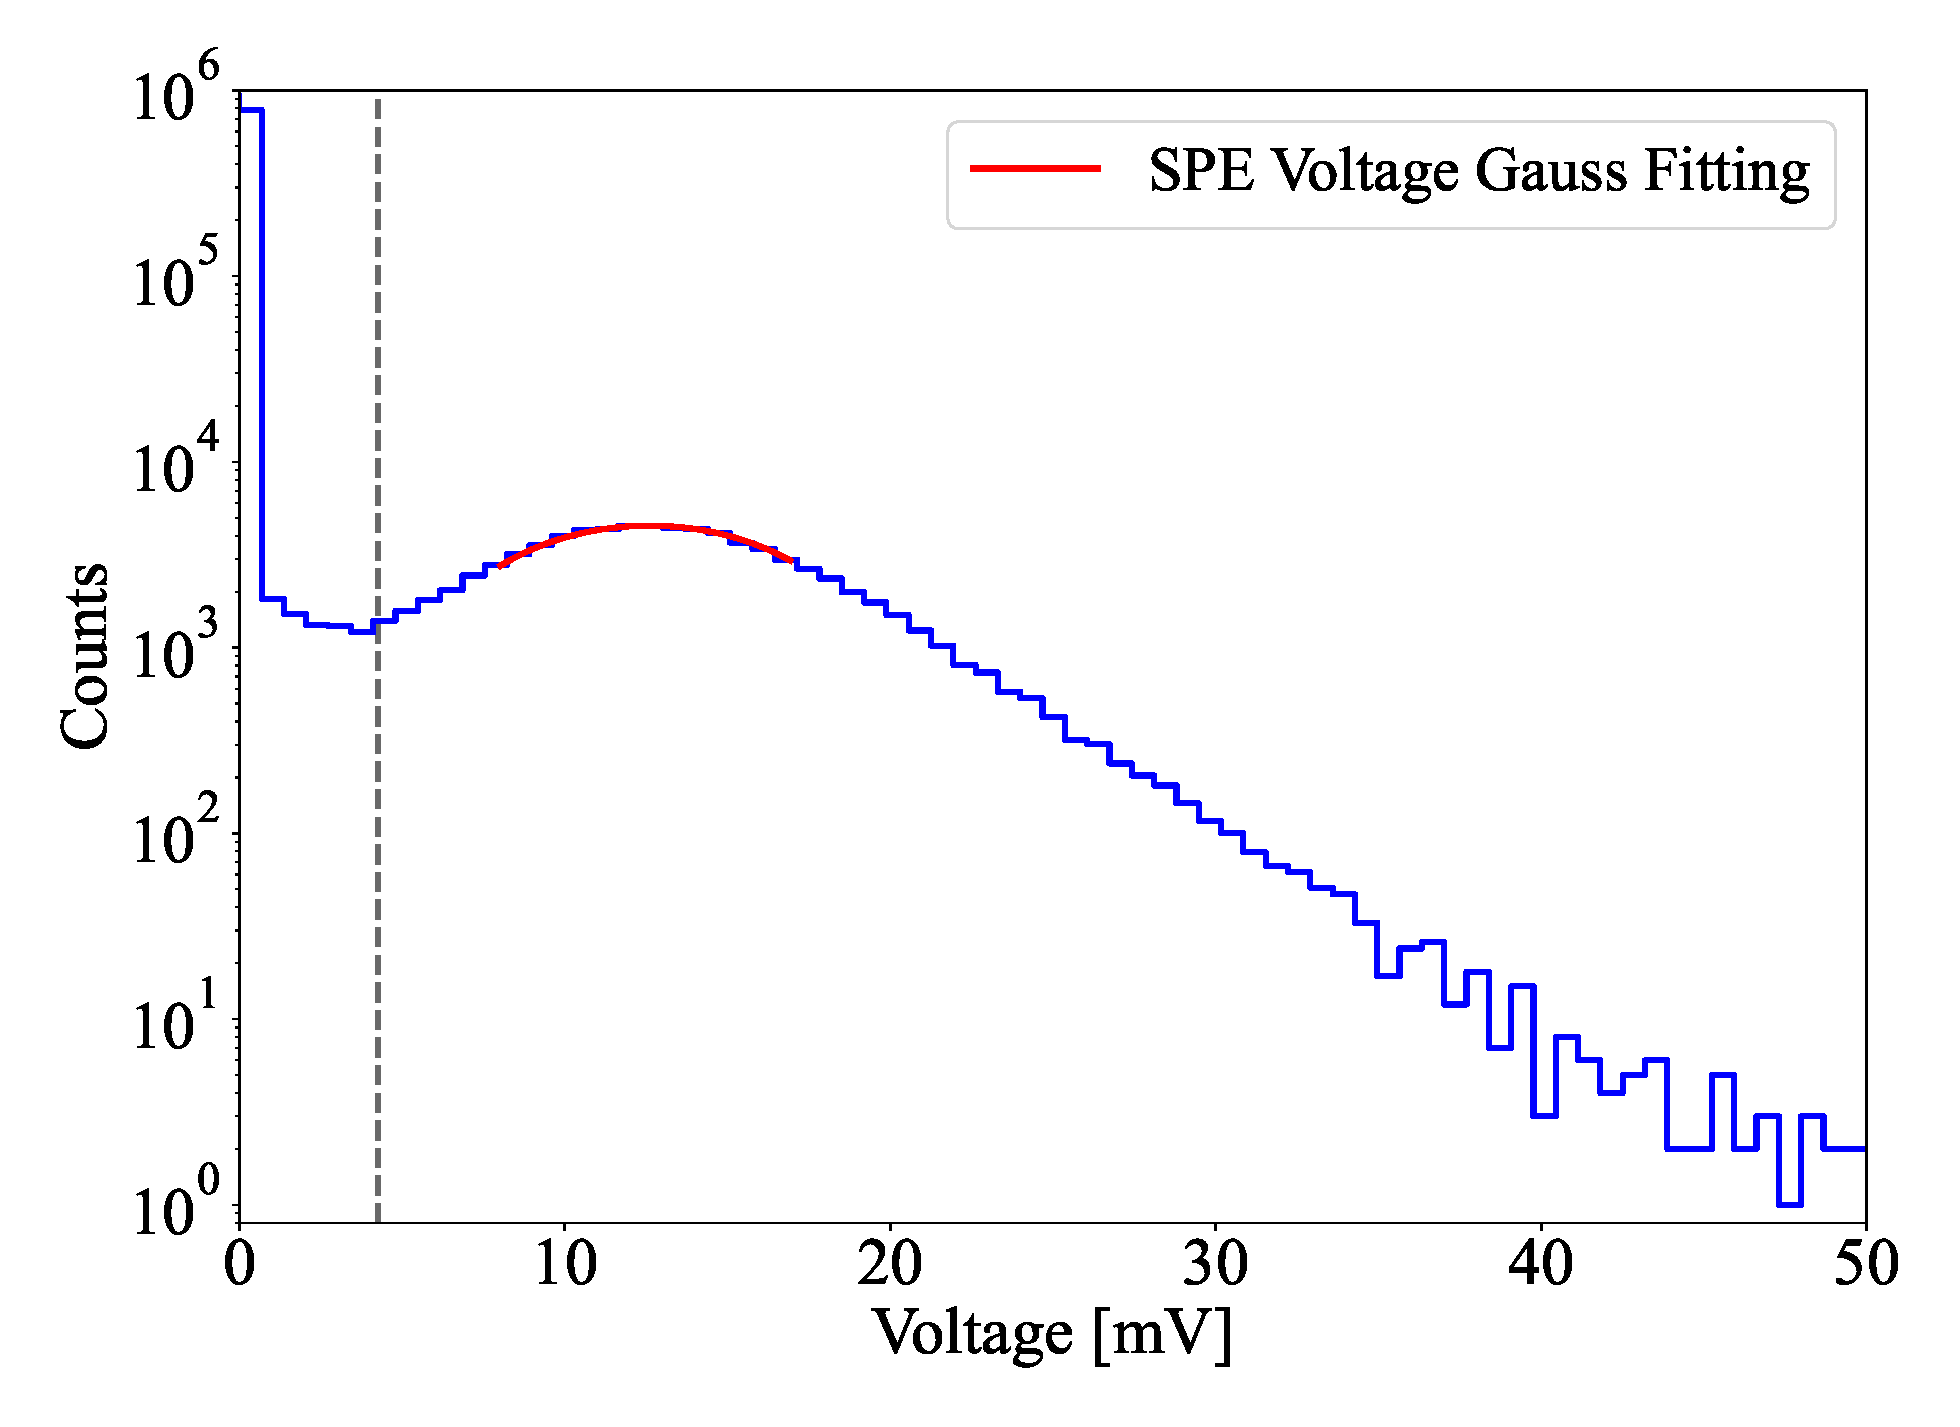
\includegraphics[width= 0.80\textwidth]{img/pmt_peak_voltage_distribution.pdf}
    \caption{
    刻度实验中测量得到的PMT波形的电压峰值的分布示意图。}
    \label{fig:pmt_peak_voltage_distribution}
\end{figure}

\begin{figure}[!hb]
    \centering
    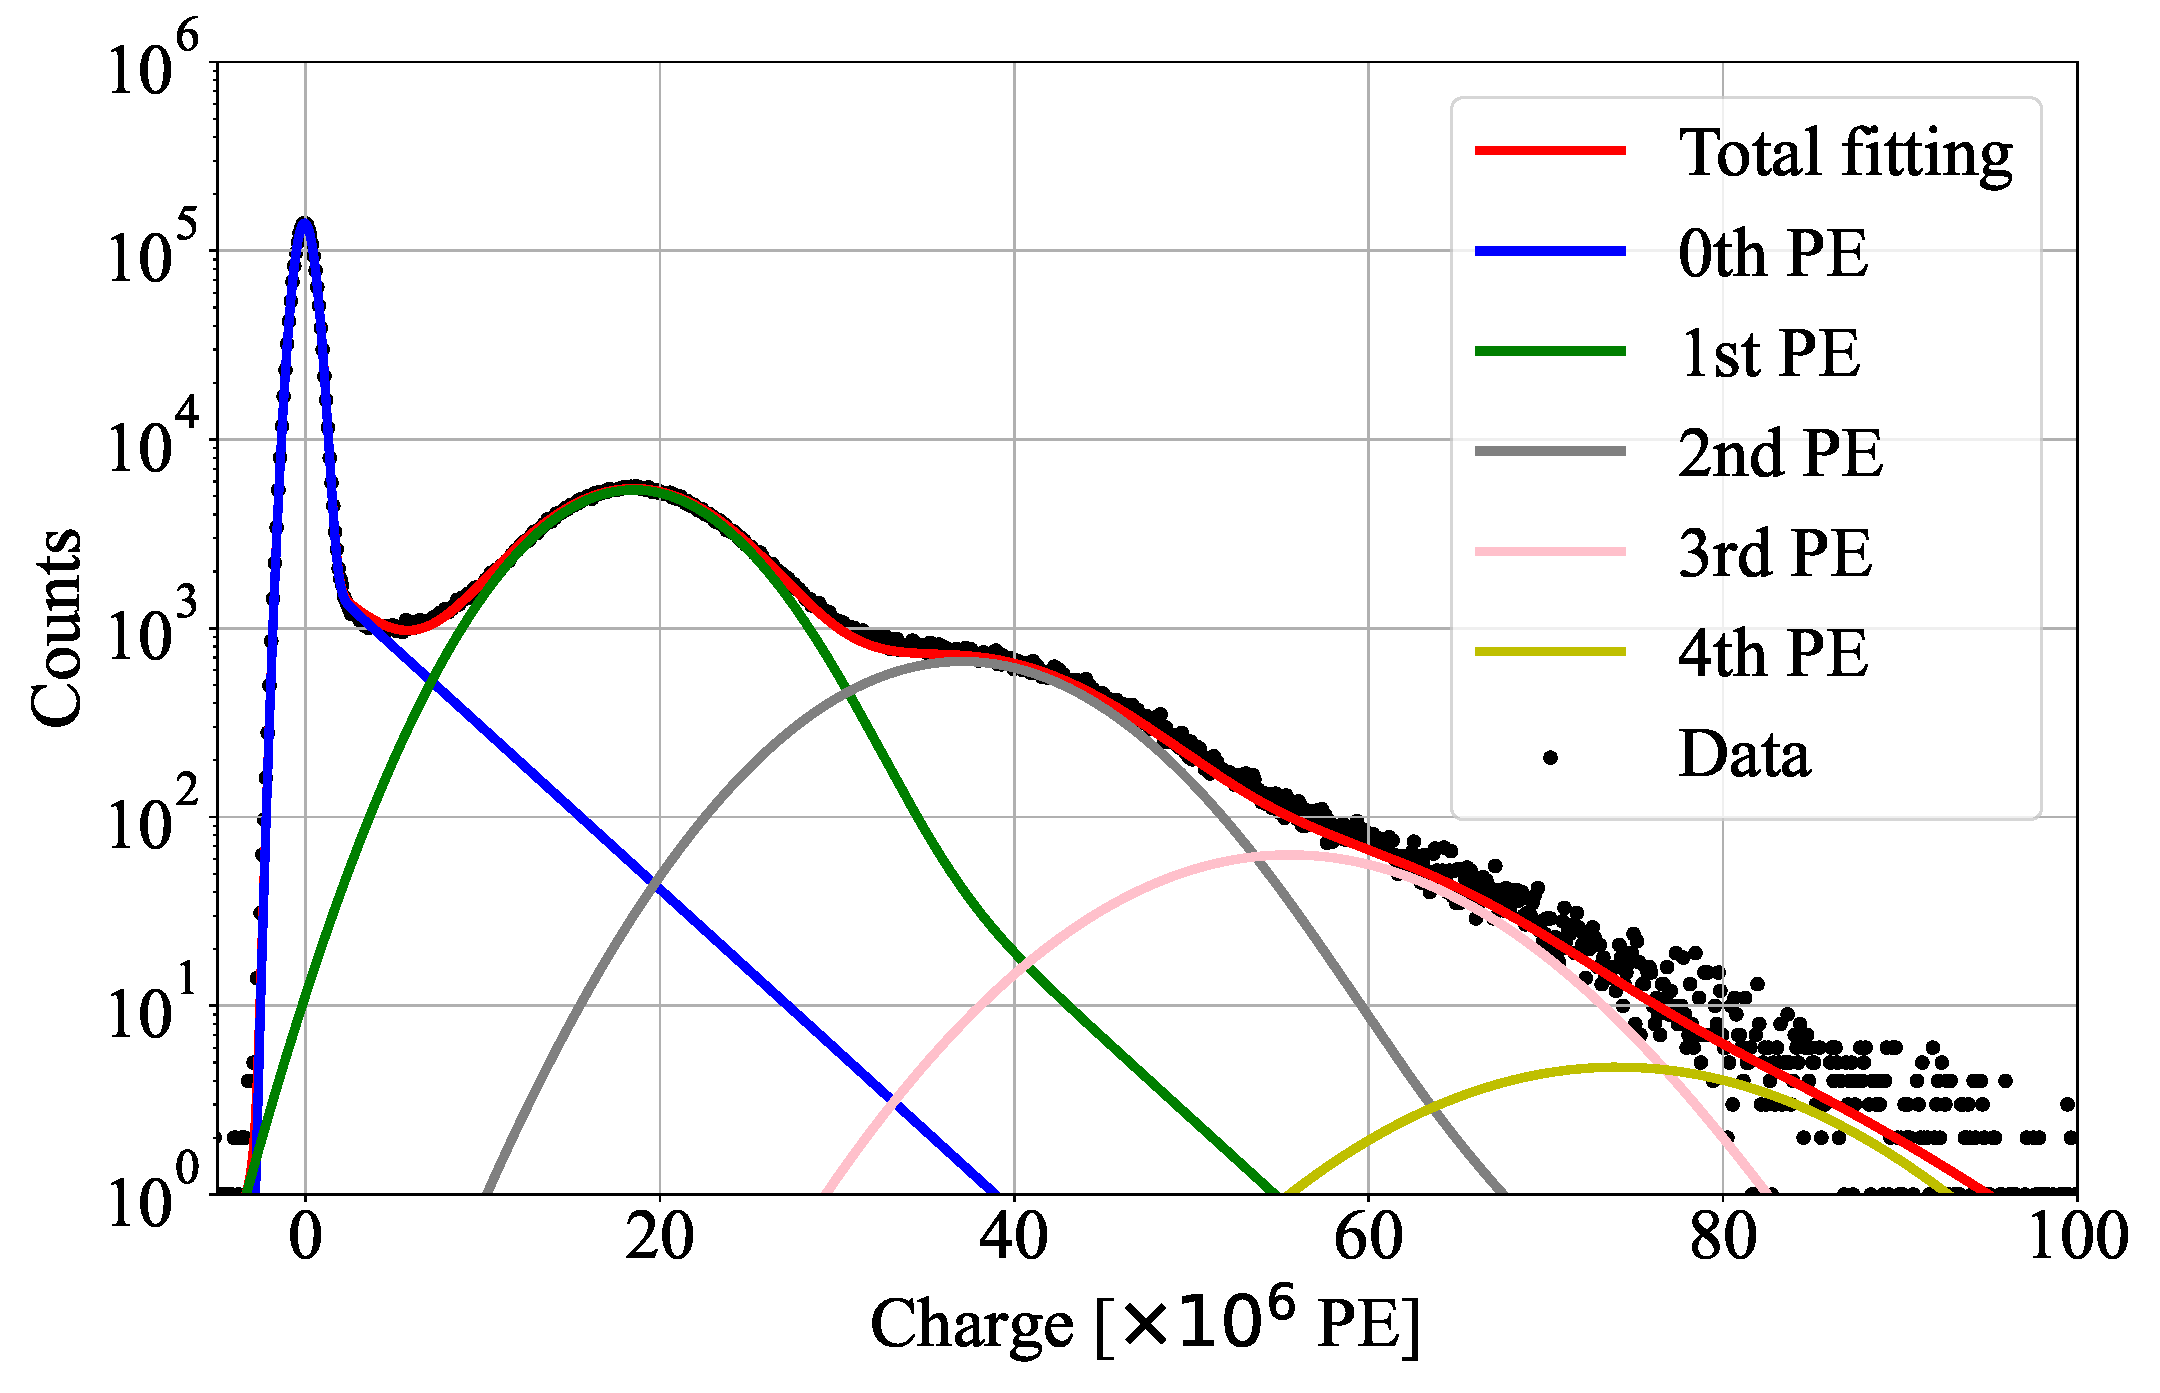
\includegraphics[width=0.85\textwidth]{img/pmt_charge_distribution.pdf}
    \caption{
    以4号PMT为例,展示的PMT测量得到的电荷的分布以及对应的拟合曲线。}
    \label{fig:pmt_charge_distribution}
\end{figure} 

测量单光子的响应对于理解PMT的性能是非常重要的,因为在探路者实验和中微子望远镜实验中,接收到的大多数信号都是单光子信号。
为了确定SPE波形的振幅,我们测量了波形峰值的分布,其结果如图\ref{fig:pmt_peak_voltage_distribution}中所示。
SPE波形的振幅可以通过用一个高斯函数来拟合波形峰值分布中的第一个峰来得到。

PMT的增益可以通过拟合PMT最终输出的电荷的分布来得到,电荷可以由ADC采样得到的波形积分得到:
\begin{equation}
    G = \sum_{i}\frac{V_i \cdot \delta t}{R \cdot e} ,
\end{equation}
其中$V_i$表示ADC测量得到的第$i$个记数点的电压值,$R = 50 \,\Omega$表示ADC的电阻,$\delta t = 4 \,\mathrm{ns}$表示采样时间间隔,$e$表示电子电荷。
我们测量得到的电荷的分布如图\ref{fig:pmt_charge_distribution}中所示。

我们使用如下的模型来拟合PMT的电荷分布\cite{PMT_fit_function:1994}:
\begin{equation}
    \begin{aligned}
        f(Q) = & \sum_{n=0}^{\infty} \text{Poisson}( n , \mu ) \times \\
        & \left( (1-w) \times \frac{1}{\sqrt{2\pi} \sigma_n} e^{-\frac{(Q-Q_n)^2}{2\sigma_n^2}} + w \times  \frac{\lambda}{2} e^{ \frac{ ( \lambda \sigma_n )^2 }{2} } e^{ - \lambda ( Q - Q_n ) } \cdot \text{Erfc} \left( \frac{1}{\sqrt{2}} \left( \lambda \sigma_n - \frac{ Q - Q_n }{ \sigma_n } \right) \right) \right) .
    \end{aligned}
    \label{eq:pmt_charge}
\end{equation}
这个函数的主体是一个柏松分布,柏松分布的平均值$\mu$表示PMT平均接收到的光电子的数量。
而对于每一个固定的光电子的数量$n$,PMT最终得到的电荷数量却存在一定的不确定性,这种不确定性由高斯分布和一个指数修正的高斯分布(exponentially modified Gaussian distribution)的叠加来描述。
其中高斯分布表示正常放大的信号,其比例为$w$,而指数修正的高斯分布用于表示错误放大的信号,例如光电子没有正常经过所有的打拿极。
它们的中心值$Q_{n} = Q_{0} + n \cdot Q_{1}$,标准差$\sigma_{n} = \sqrt{\sigma_{0}^{2} + n \cdot \sigma_{1}^{2}}$。
第一个光子峰(图\ref{fig:pmt_charge_distribution}中的绿色曲线)的平均值便是PMT的增益。

\subsubsection{光子探测效率}

在海铃探路者实验的PMT系统中,我们通过测量远近两个接收球中的光电子的平均数比值来推导海水中光的衰减长度。因此,我们必须扣除发光球两个面的相对亮度以及接收球中的PMT的相对探测效率的影响,而这两个量可以在刻度实验中测量得到。

\begin{figure}[ht]
    \centering
    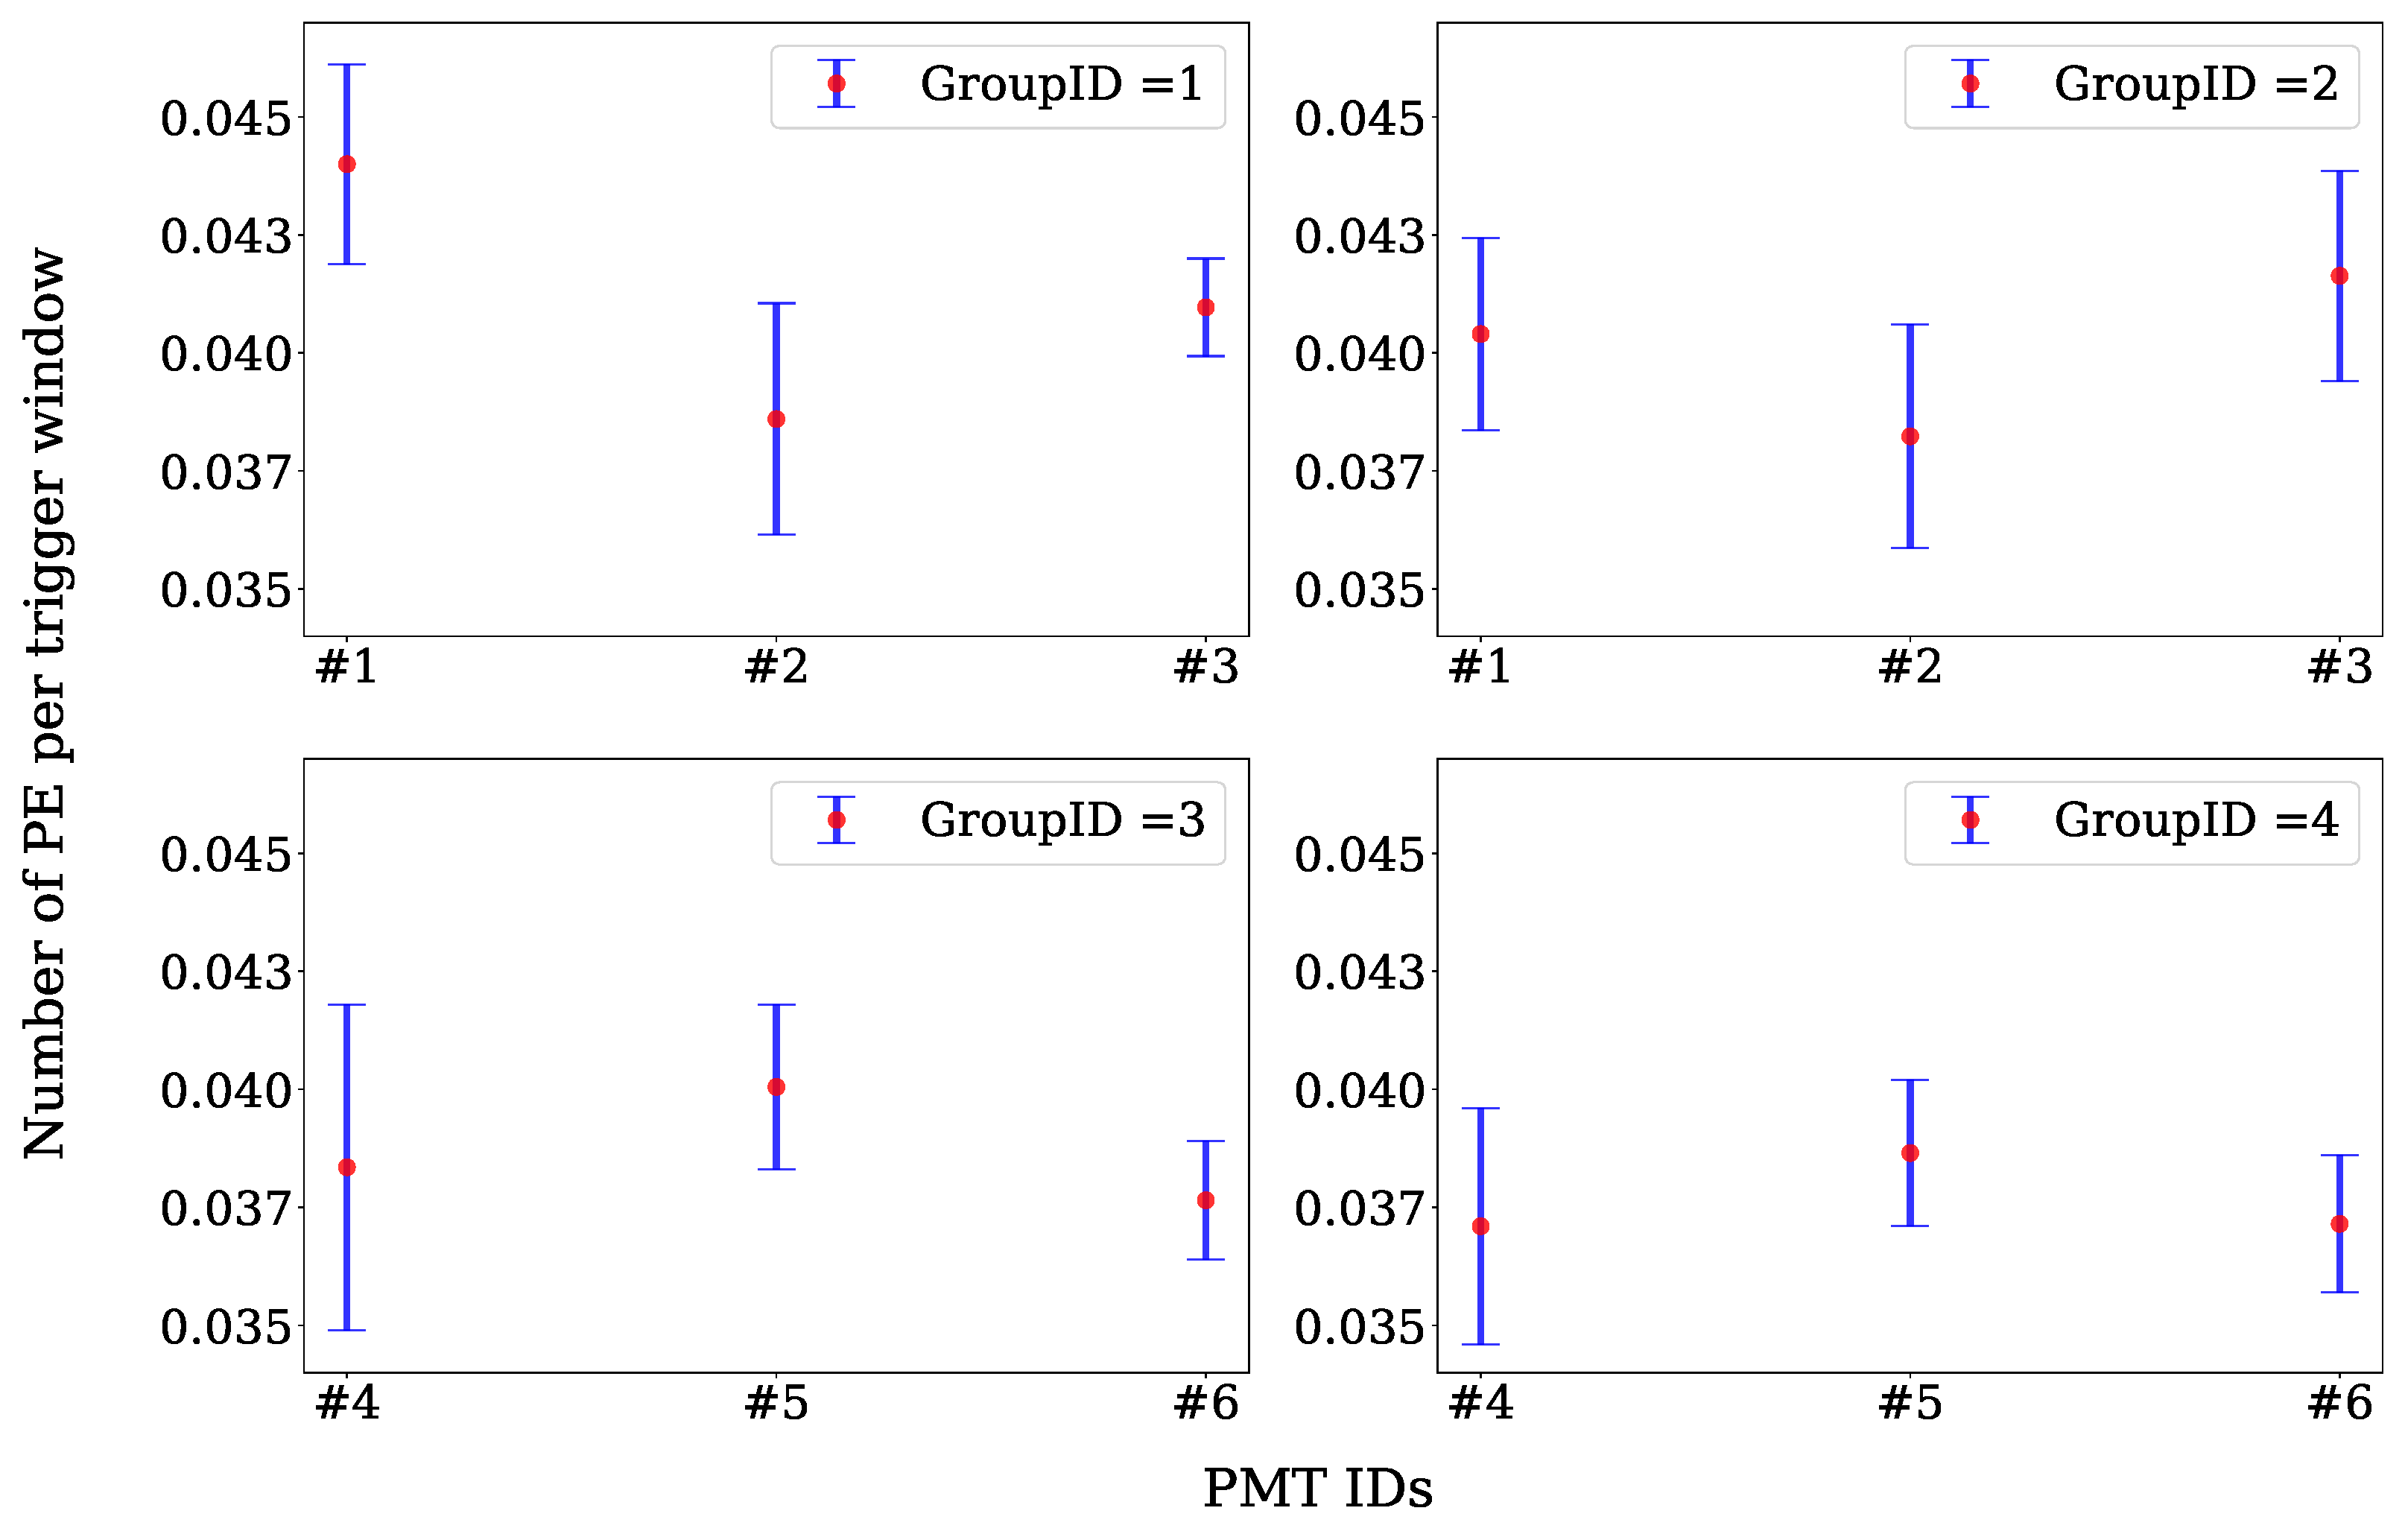
\includegraphics[width = 0.98\textwidth]{img/pmt_relative_photon_efficiency.pdf}
    \caption{不同配置下的探测器的各个PMT平均接收到的光子数量。}
    \label{fig:pmt_relative_photon_efficiency}
\end{figure}

在各个不同的测试配置下,PMT接收到的平均光子数可以通过拟合\ref{eq:pmt_charge}中的$\mu$值得到,其结果如图\ref{fig:pmt_relative_photon_efficiency}中所示。
如果我们把发光球的A/B两面测量得到的结果进行平均,并且以4号PMT作为基准,那么各个PMT的相对探测效率如图\ref{fig:pmt_relative_detection_eff_ave}中所示。

\begin{figure}[!ht]
    \centering
    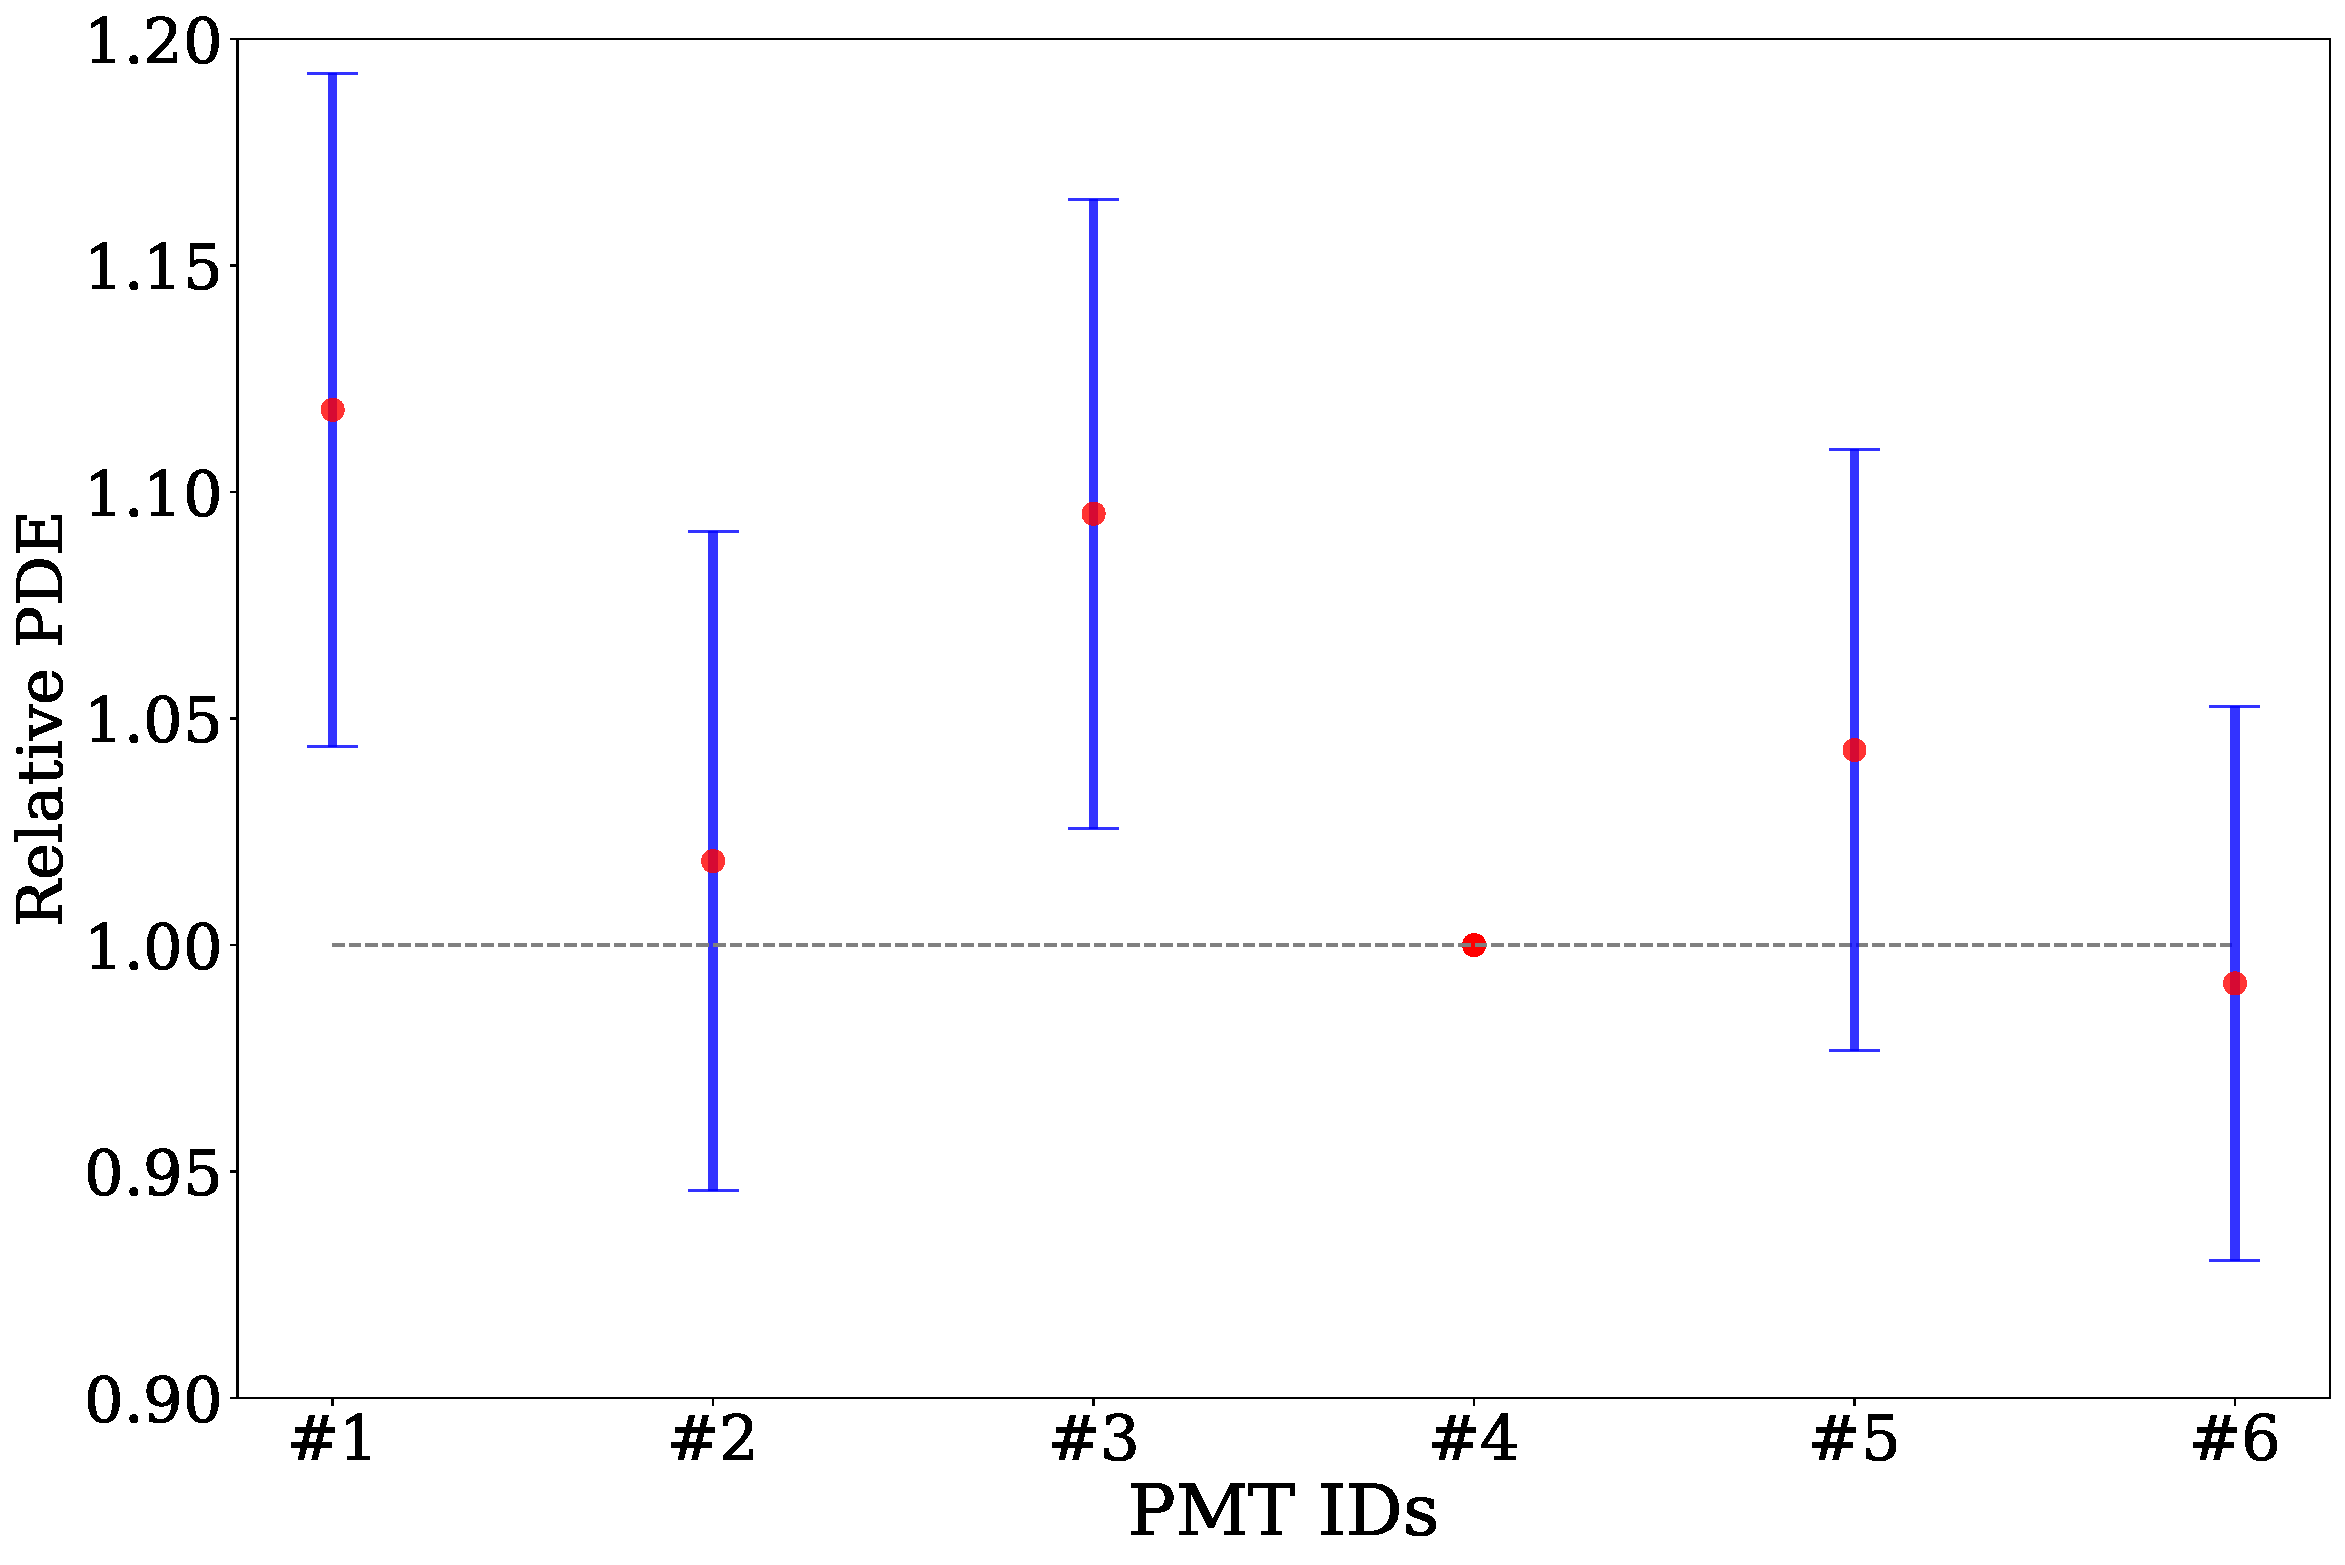
\includegraphics[width = 0.75\textwidth]{img/pmt_relative_detection_eff_ave.pdf}
    \caption{各个PMT相对于4号PMT的相对光子探测效率。}
    \label{fig:pmt_relative_detection_eff_ave}
\end{figure}

\begin{figure}[!ht]
    \centering
    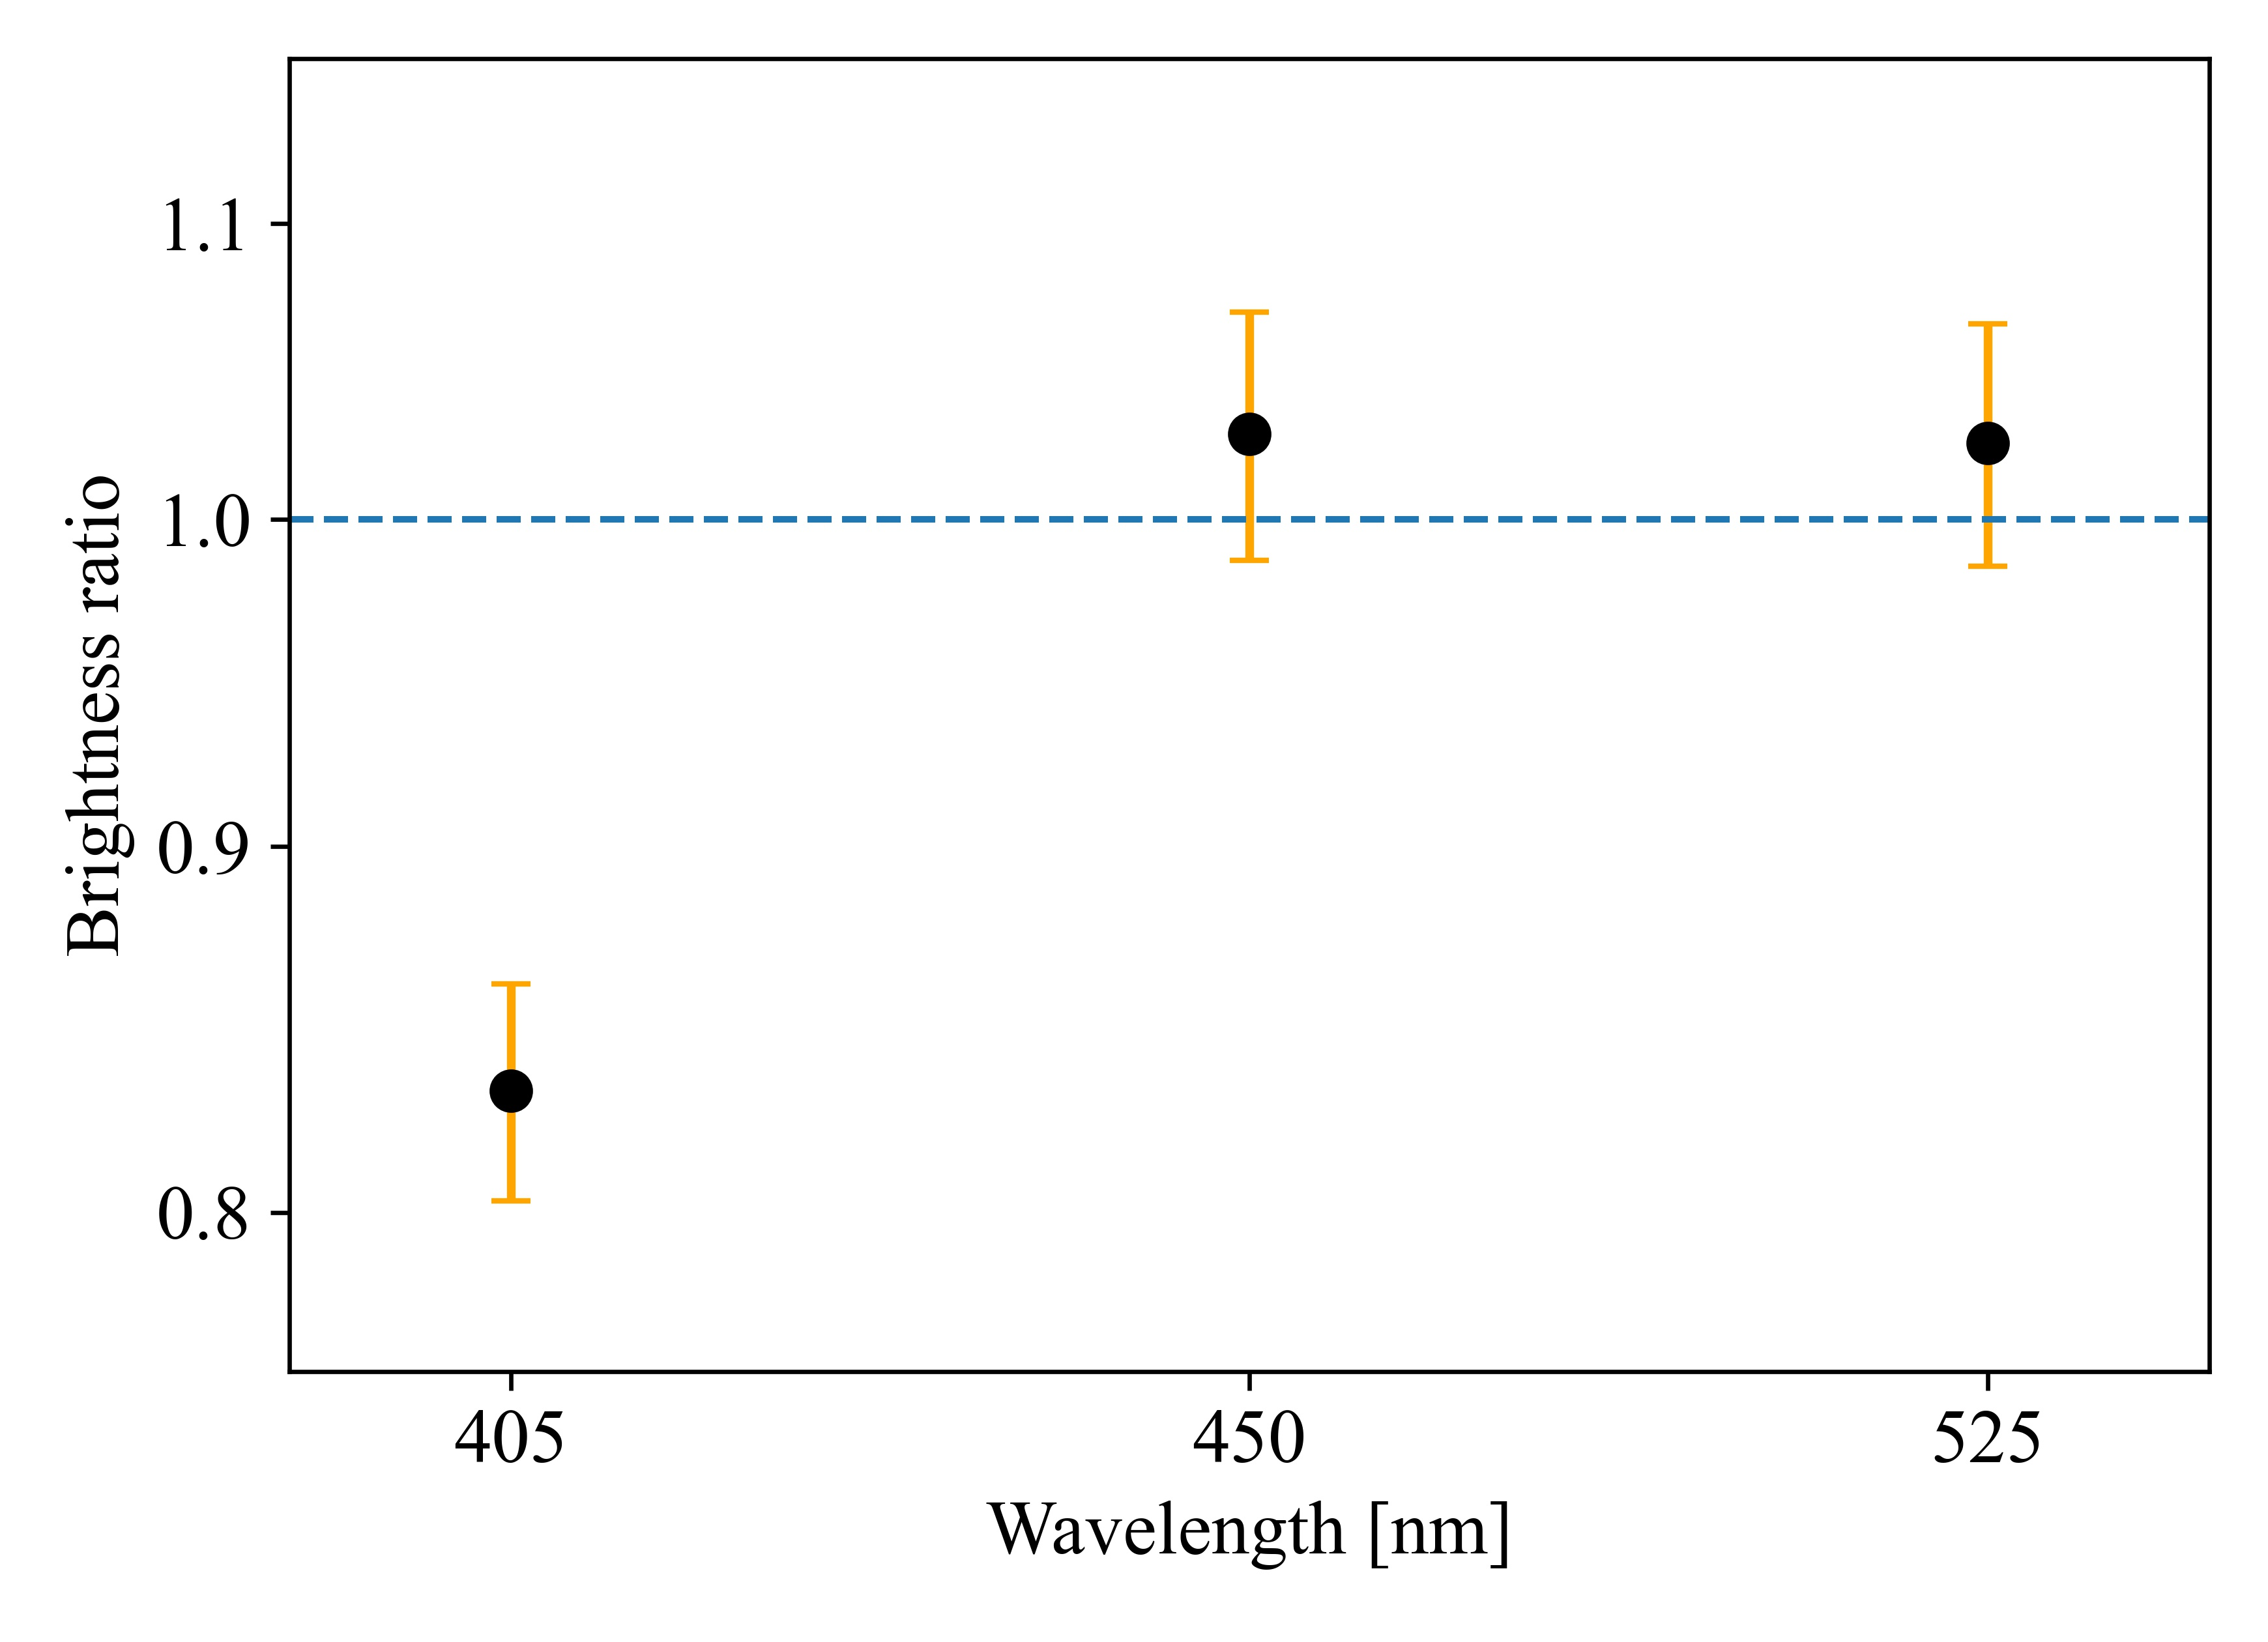
\includegraphics[width = 0.75\textwidth]{img/led_brightness_ratio.jpg}
    \caption{发光球的A/B两面的发光强度在不同波长下的比值。}
    \label{fig:led_brightness_ratio}
\end{figure}

通过分析图\ref{fig:pmt_relative_photon_efficiency}中不同的配置结果,我们可以测量得到的发光球的A/B两面的发光强度在不同波长下的比值,其结果如图\ref{fig:led_brightness_ratio}中所示。




\subsubsection{空气中的光子到达时间分布}

正如我们在章节\ref{sec:pathfinder_sim}中讨论的那样,PMT系统通过测量光子到达时间的延后来解码海水中的散射性质。
但是除了散射以外,光子到达时间还受到LED发光的脉冲宽度,光电子在PMT中的渡越时间的影响。
我们可以在刻度实验中对这两项因素进行详细测量。

我们在不同的配置下测量最终PMT的光子到达时间,对于4号PMT,其到达时间的分布如图\ref{fig:pmt_arrival_time_distribution_cali}中所示。

\begin{figure}[htb]
    \centering
    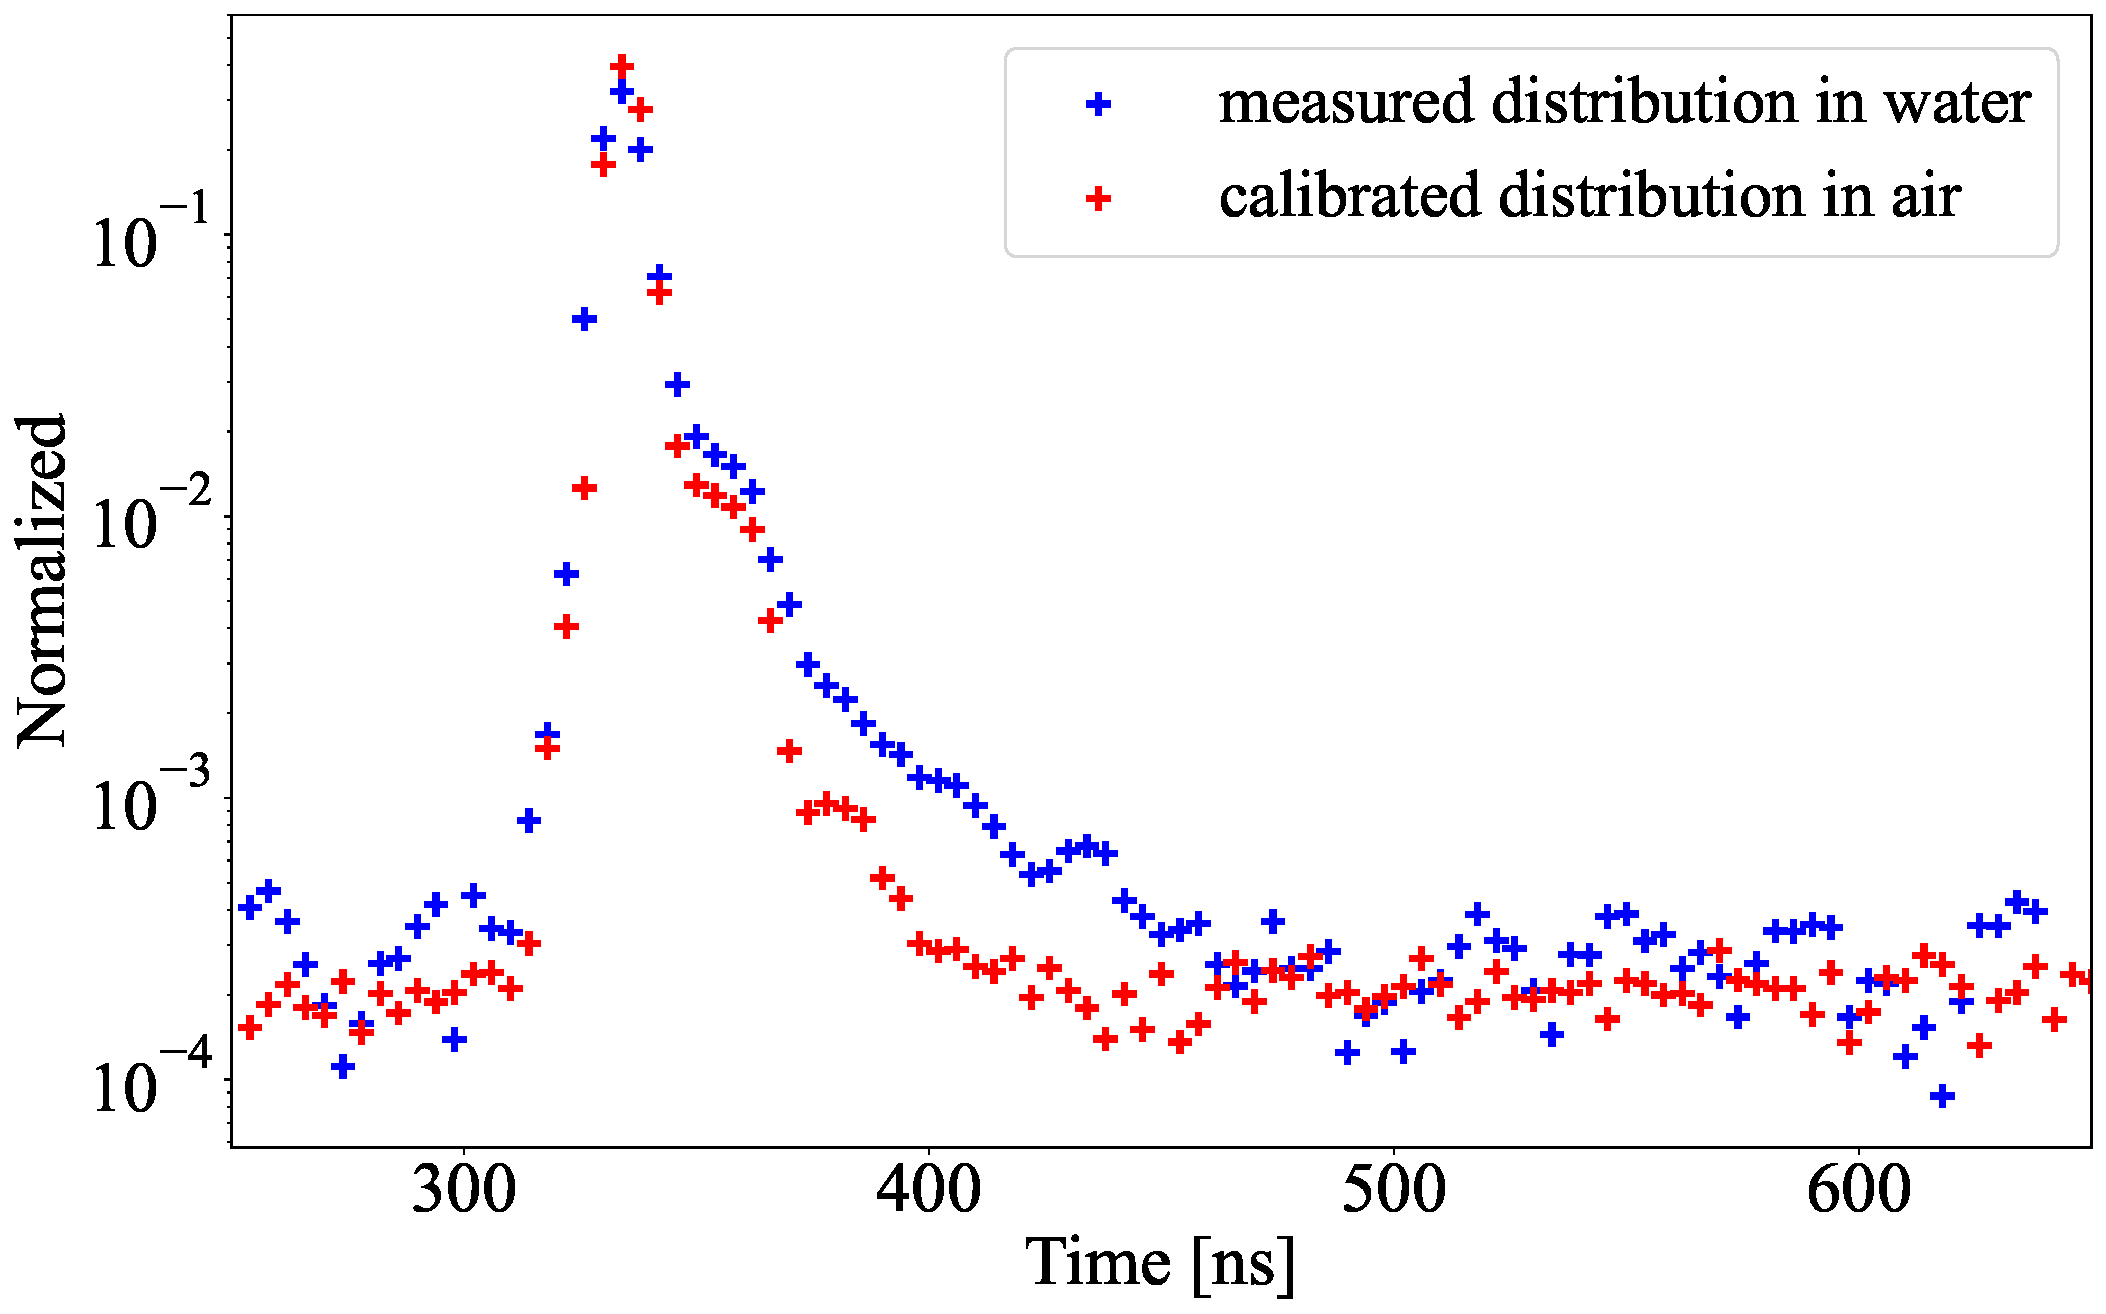
\includegraphics[width=0.86\textwidth]{img/pmt_arrival_time_distribution_cali.pdf}
    \caption{空气刻度中(红色)和探路者实验中(蓝色)测量得到的光子到达时间的分布的对比图。其中我们把时间进行了平移,使得到达时间分布的上升沿能够对上。}
    \label{fig:pmt_arrival_time_distribution_cali}
\end{figure}

\section{光学性质的测量结果}

\subsection{等效衰减长度的测量}

在实验测试中,我们可以定义等效衰减长度$\lambda_\mathrm{att,eff}$。它的物理意义不同于\ref{sec:pathfinder_sim}中的$\lambda_\mathrm{att}$或者是$\lambda_\mathrm{att,avg}$,是一个用于表示经过一段距离的衰减后,PMT实际接收到的总光子数的量:
\begin{equation}
    N_{\text{recv}} = N_{\text{emit}} \cdot \frac{A_{\text{recv}}}{2\pi d^{2}} \cdot e^{-\frac{d}{\lambda_{\text{eff, att}}}} \cdot \eta_{\text{recv}} ,
    \label{eq:eff_att}
\end{equation}
其中$N_{\text{recv}}$是PMT接收到的总光子数量,$N_{\text{emit}}$是LED发射的总光子数量,$d$表示传播距离,$A_{\text{recv}}$表示PMT接收光子面积,$\eta_{\text{recv}}$表示PMT的相对光子接收效率。

在我们的海铃探路者实验中,我们采用对比远近两个距离下PMT接收到的光子数的相对比值的方法来实现对等效衰减长度的测量:
\begin{equation}
   \lambda_{\text{eff,att}} = (d_n - d_f) /\ln{(\frac{N_{\text{recv},n}}{N_{\text{recv},f}} \frac{N_{\text{emit},f}}{N_{\text{emit},n}} \frac{d_n^2}{d_f^2} \frac{\eta_n}{\eta_f})},
   \label{eq:eff_att_measure}
\end{equation}
其中$N_{\text{emit},f}/N_{\text{emit},n}$表示发光球面对远处和近处的两个面的相对亮度比值,其刻度结果如图\ref{fig:led_brightness_ratio}中所示。而$\frac{\eta_n}{\eta_f}$表示远处和近处的的一对PMT的相对光子探测效率,其刻度结果如图\ref{fig:pmt_relative_detection_eff_ave}。
PMT系统通过公式\ref{eq:eff_att_measure}得到的的海水的等效衰减长度测量结果如图\ref{fig:pathfinder_op_result}中黑色圆点所示。
对于相机系统而言,它对衰减长度更加灵敏,但也可以通过一些修正方法,来获得与PMT测量的等效衰减长度定义相接近的量,其测量结果如图\ref{fig:pathfinder_op_result}中黑色方块所示,具体的测量方法参见\cite{pathfinder_camera:2022}。

\begin{figure}[htbp]%
    \centering
    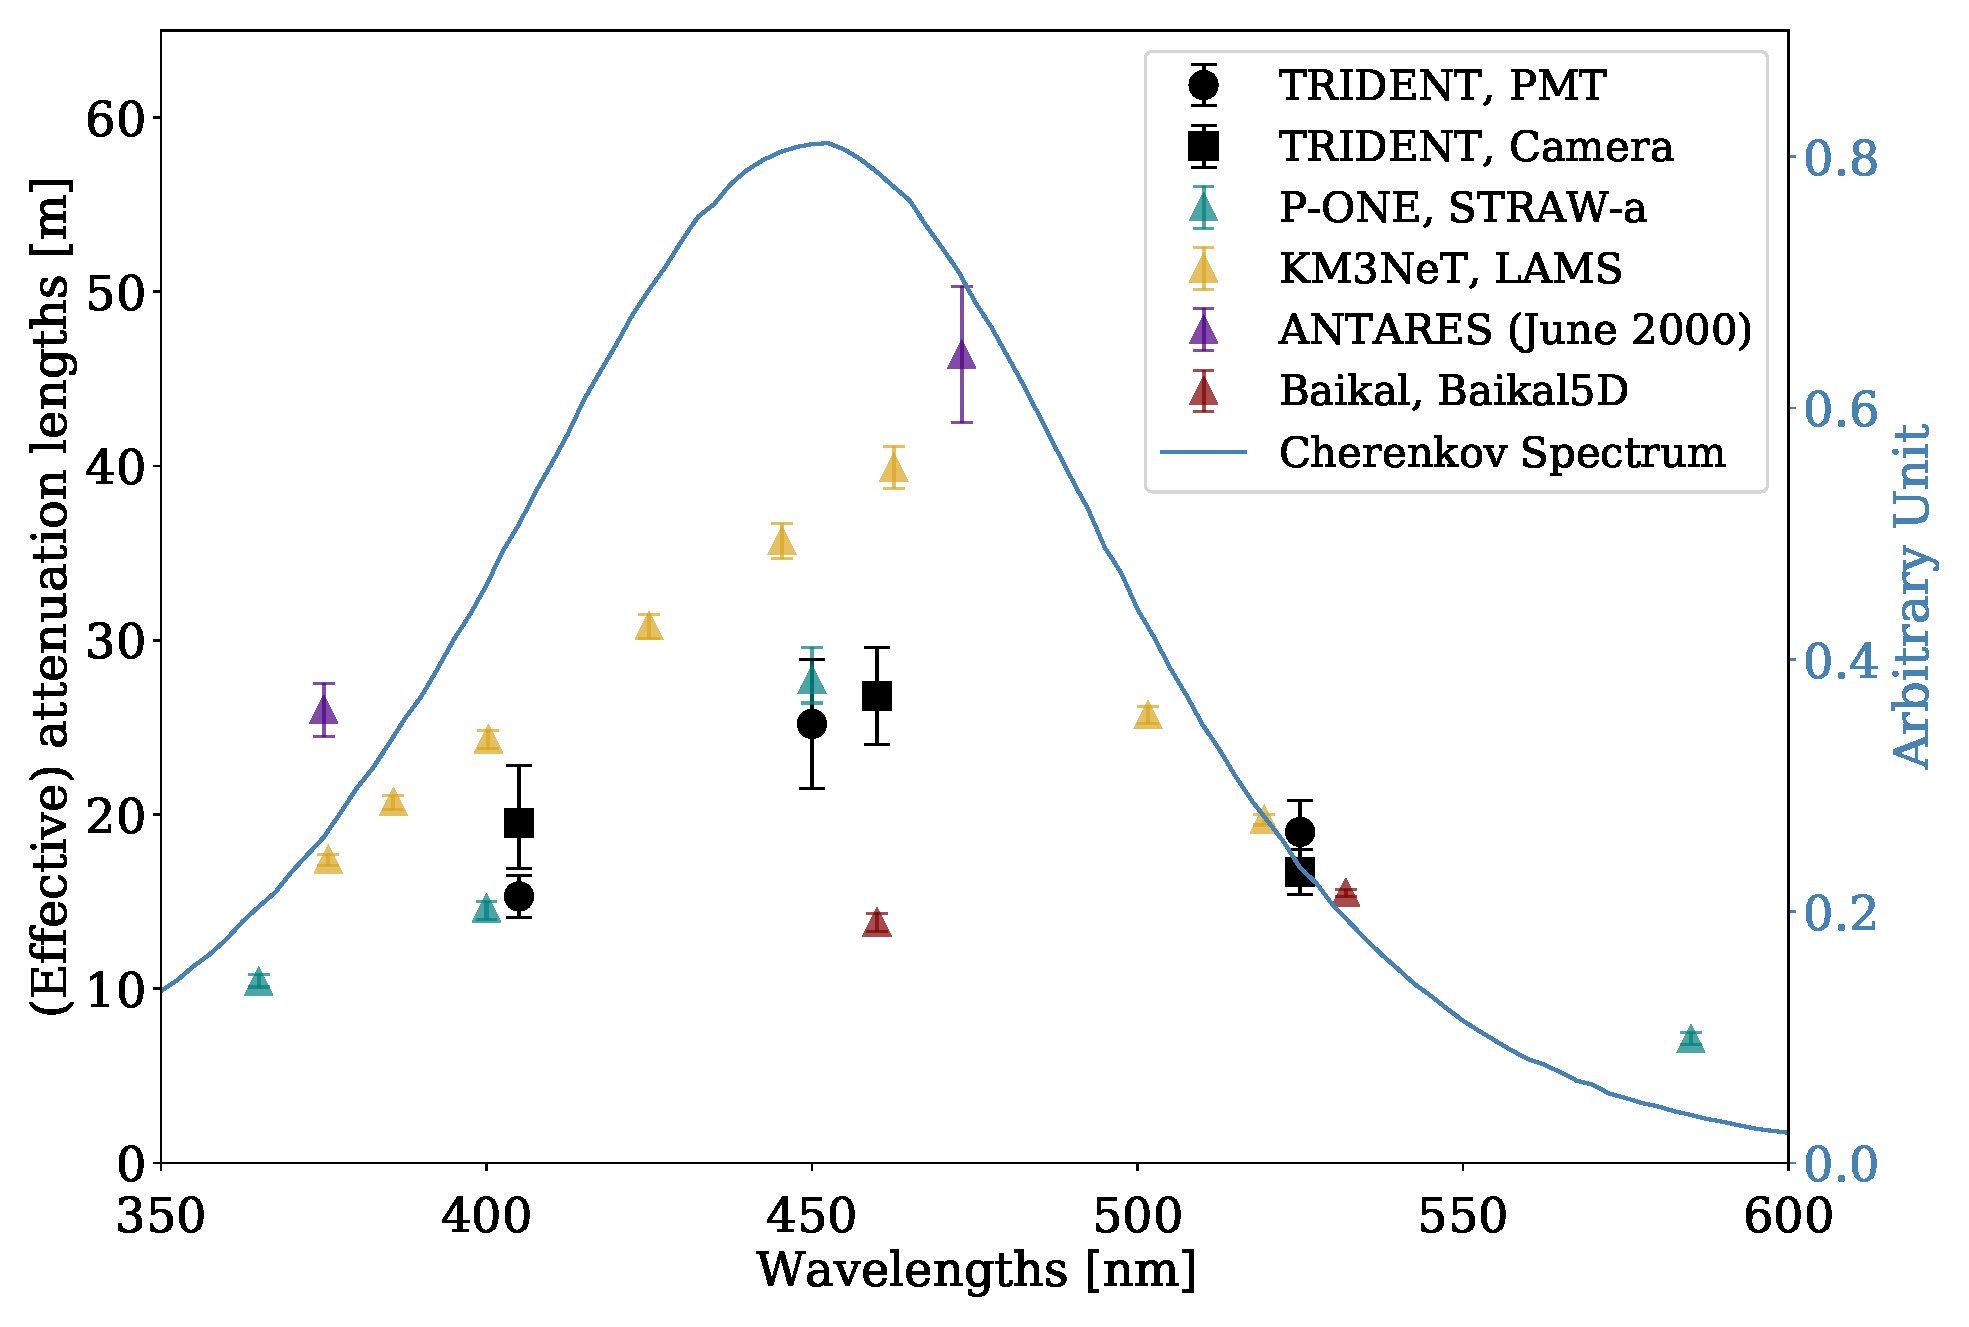
\includegraphics[width=0.98\textwidth]{img/pathfinder_op_result.pdf}
    \caption{海铃选址处的深海海水的等效衰减长度在三种不同的波长($405\,\mathrm{nm}$,$450/460\,\mathrm{nm}$和$525\,\mathrm{nm}$)下通过在两套独立的系统——PMT系统(黑色圆点)和相机系统(黑色方框)下的测量结果。
    同时图中也展示了KM3NeT\cite{OP_KM3NeT_LAMS:2011},P-ONE\cite{OP_P-One:2021},ANTARES\cite{OP_ANTARES:2004}和Baikal-GVD\cite{OP_Baikal:2012}望远镜选址处的测量结果用于比较。
    在探路者项目中测量的光学性质输入下,海铃中微子望远镜中的探测模块探测到的切伦科夫光的波长分布被用蓝线表示了出来。}
    \label{fig:pathfinder_op_result}
\end{figure}

\subsection{精细光学参数的测量}

除了上一节中介绍的对等效衰减长度的直接测量外,我们还利用PMT系统对章节\ref{sec:pathfinder_sim}中所讨论的各项详细的光学性质进行了测量,这是通过构建完整的到达时间分布的模拟来实现的:
\begin{equation}
\begin{aligned}
    \frac{\mathrm{d}N_\mathrm{recv}}{\mathrm{d}t} & =
    [ N_{\mathrm{emit}} \times f(t) ] \\
    & \otimes [ \frac{A_\mathrm{recv}}{4 \pi d^2} \times P_\mathrm{prop}( t \,\vert\, \lambda_\mathrm{abs} , \lambda_\mathrm{Ray} , \lambda_\mathrm{Mie} , \left \langle \cos\theta \right \rangle , n , d ) ] \\
    & \otimes [ \eta_\mathrm{recv} \times g(t) ] ,
    \label{eq:arrival_time_distribution}
\end{aligned}
\end{equation}
其中$f(t)$和$g(t)$分别表示LED发光和PMT接收光子的时间响应能力,其刻度结果如图\ref{fig:pmt_arrival_time_distribution_cali}中所示,而$P_\mathrm{prop}( t \,\vert\, \lambda_\mathrm{abs} , \lambda_\mathrm{Ray} , \lambda_\mathrm{Mie} , \left \langle \cos\theta \right \rangle , n , d ) ]$表示光子在海水中传播时,由于光子的散射所导致的时间弥散,它可以通过模拟得到。

为了将实验测量的结果与由公式\ref{eq:arrival_time_distribution}中得到的模拟加上刻度的结果进行对比,我们构建了$\chi^2$来作为衡量标准:
\begin{equation}
    {\chi}^2 = \sum_{i=1}^{N}{ \frac{ ( D_i - M_i - \sum_{k=1}^{K}{ c_k \cdot \beta_{ki} } )^2 }{ {\sigma_i}^2 } } + \sum_{k=1}^{K}{ {c_k}^2 } , 
    \label{eq:ATD_chi_square_fit}
\end{equation}
其中$D_i$表示实验测量到的每一个时间区间内的到达光子数,$M_i$表示模型预测结果,即光子传播模拟和刻度实验的叠加结果。
非关联误差项$\sigma_i$包含了数据的统计涨落,电子学噪声以及LED发光和PMT响应的时间分布的不确定性。
关联误差项$\beta_{ki}$以及每一项对应的不确定度$c_k$包含LED的发光亮度和PMT相对量子效率,发光球与接收球之间的距离的测量误差,此外还包含了由于$4\,\text{ns}$的ADC测量时间分辨率导致的额外误差。

通过不停地改变模拟中输入的光学性质参数得到不同的模拟的到达时间分布,我们可以对公式\ref{eq:ATD_chi_square_fit}定义的${\chi}^2$求最小值,通过这样的方法,我们可以测量得到\ref{subsec:optical_model}中定义的详细光学参数:$\lambda_\mathrm{abs}$,$\lambda_\mathrm{Ray}$,$\lambda_\mathrm{Mie}$,$\mu$。在蓝光波段的测量结果如表\ref{tab:optical_property_blue}中所述,对其他波段的测量结果参见\cite{TRIDENT_pathfinder:2022}。

\begin{table}[htpb]
\renewcommand{\arraystretch}{1.8}
\setlength{\arrayrulewidth}{0.15mm}
\setlength{\doublerulesep}{0.55mm}
\centering
    \begin{tabular}{|c|c|c|c|c|c|c|}
      \hline
      \multicolumn{7}{|c|}{PMT (at $\sim$ 450 nm, $\sim$ 50 minutes)} \\
      \hline
      Method & $\lambda_{\text{abs}}$ [m] & $\lambda_{\text{ray}}$ [m] & $\lambda_{\text{mie}} $[m] & $\cos \theta_{\text{mie}}$ & $\lambda_{\text{att}}$ [m] & $\lambda_{\text{att,eff}}$ [m] \\   
      \hline
      $\chi^2$ fitting & $ 27.4 ^{+1.1}_{-0.9}$ & $ 200 ^{+13}_{-10}$ & $ 84^{+12}_{-8}$ & $0.97 ^{+0.02}_{-0.02}$ & $18.7^{+3.0}_{-2.1}$ & \multirow{2}{*}{$25.2\pm 3.7$} \\ 
      \cline{1-6}
      MCMC & $26.4^{+1.2}_{-1.0}$ & $203^{+15}_{-11}$ & $64^{+12}_{-14}$ & $0.97^{+0.01}_{-0.01}$ & $17.2^{+0.8}_{-1.3}$ & {} \\
      \hline
      \multicolumn{7}{|c|}{Camera (at $\sim$ 460 nm, $\sim$ 8 minutes)} \\
      \hline
      Method & $\lambda_{\text{abs}}$ [m] & \multicolumn{3}{c|}{$\lambda_{\text{sca}}$ [m]} & $\lambda_{\text{att}}$ [m] & $\lambda_{\text{att,eff}}$ [m] \\ 
      \hline
      $\chi^2$ fitting & $26.5\pm0.5$ & \multicolumn{3}{c|}{$62.9\pm3.7$} & $18.7\pm0.2$ & \multirow{2}{*}{$26.8\pm 2.8$} \\ 
      \cline{1-6}
      $I_{\text{center}}$ &   \multicolumn{5}{c|}{$\lambda_{\text{att}} = 19.3 \pm 1.3$}  & {} \\
      \hline
    \end{tabular}
    
    \caption{在$3420~\mathrm{m}$深的海水,各项光学性质的详细测量结果。其中PMT系统测量的是$450~\mathrm{nm}$的光源,而相机系统测量的是$460~\mathrm{nm}$的光源。每次测量的采数时间也同样被注释在表中。}
    \label{tab:optical_property_blue}
\end{table}
